This chapter addresses the validity of instruction reordering under the ECMAScript memory model.
We first start by showing some examples of Candidate Executions where reordering is not safe in the relaxed memory context.  
We give a brief summary of our approach towards a proof to identify when such a reordering is safe.
Next, we introduce few more definitions for our purpose followed by two lemmas that will be instrumental for proofs in this chapter and the next. 
We then formulate a theorem and a corresponding corollary that covers validity of reordering at a Candidate Execution level. 
Lastly, we address reordering at the program level involving conditional branching and loops.
We use counter examples to give a better intuitive understanding of the elements of the proof.
\ \newline
\ \newline  
\hrule 
\ \newline 
\ \newline 


\section{Introduction}
    Instruction reordering is a common transformation done by the compiler/hardware, which is essential to optimizations such as instruction scheduling, loop invariant removal, partial redundancy elimination, etc. 
    However, whether we can do such reordering freely given a concurrent program using relaxed memory accesses is a bit unclear. 
     
    \paragraph{Simple reordering is not straightforward under shared memory semantics}
    The main reason is that memory accesses here, do not just perform the desired operation (i.e Read / Write) but also imply certain visibility guarantees across all the other threads.  
    In our observation, we find that, the relaxed memory model of ECMAScript prescribe semantics for visibility using the $\stck{_{hb}}$ relations. 
    
    \paragraph{Some Examples}
        We show a couple of examples to showcase why reordering may not be that straightforward. 
        Consider the first example in Figure~\ref{reord:example1(a)} below of a Candidate before and after reordering two events.
        The original candidate is to the left and that on the right is after reordering the two reads of $T2$.
        The observable behavior in question is written in the middle(orange box). 
        \begin{figure}[H]
            \centering
            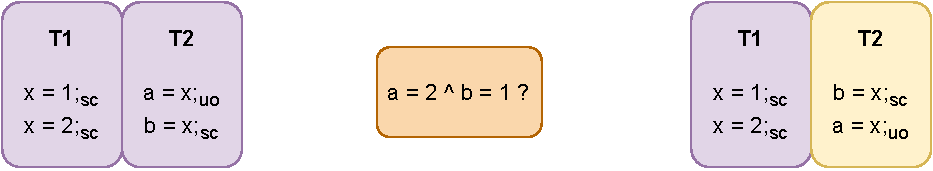
\includegraphics[scale=0.7]{5.InstructionReordering/0.Intro/ReorderingExample1(a).pdf}
            \caption{First example for reordering in candidates of the original program and its reordered counterpart.}
            \label{reord:example1(a)} 
        \end{figure}
        
        Figure~\ref{reord:example1(b)} has two sets of relations. 
        The first justifies the outcome for the reordered Candidate. 
        While the second justifies for the original Candidate. 
        Notice that in the first set of relations, we can infer that one may have a read memory ordered before a write that it reads from. 
        This is quite counter intuitive to understand at first. 
        But strictly from the semantics of the model, this justification to the observable behavior is completely valid\footnotemark. 
        \begin{figure}[H]
            \centering
            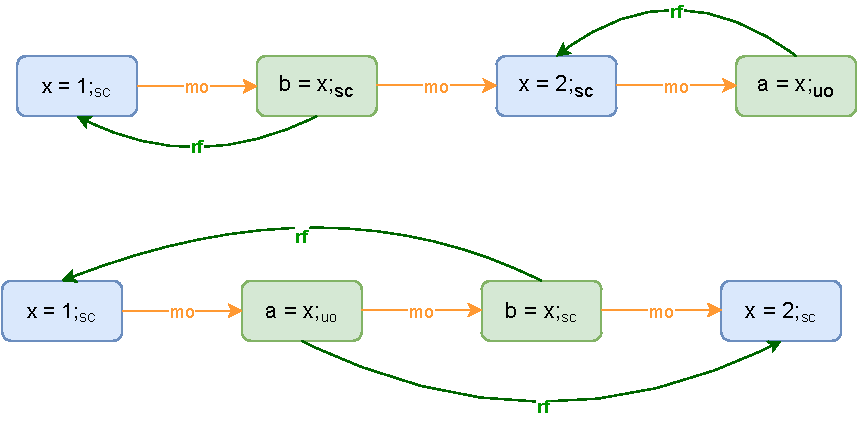
\includegraphics[scale=0.7]{5.InstructionReordering/0.Intro/ReorderingExample1(b).pdf}
            \caption{The set of partial order relations justifying the observable behavior in question for both the candidates in Figure~\ref{reord:example1(a)}.} 
            \label{reord:example1(b)}
        \end{figure}

        \footnotetext{In practice, this can be due to read speculation at the hardware level.}
        
        Consider another example in Figure~\ref{reord:example2(a)}.
        The figure on the left is the original candidate and that on the right is after reordering the two events of $T1$.
        The observable behavior in question is written in the middle(orange box). 
        \begin{figure}[H]
            \centering
            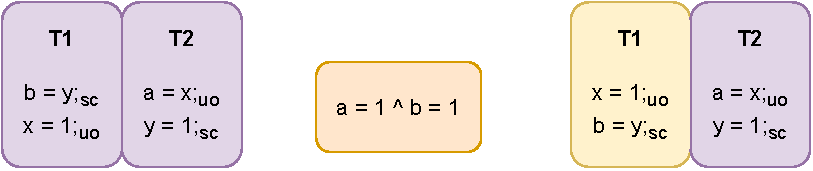
\includegraphics[scale=0.7]{5.InstructionReordering/0.Intro/ReorderingExample2(a).pdf}
            \caption{Second example for reordering with candidates of the original program and its reordered counterpart.} 
            \label{reord:example2(a)}
        \end{figure}
   
        Figure~\ref{reord:example2(b)} has two sets of relations. 
        The first justifies that such an outcome is not possible for the original program candidate due to Axiom \ref{CoRe}. 
        While the second justifies that this outcome is possible for the reordered program.
        Note that we cannot infer in the reordered candidate the set of relations for any candidate execution to have $\reln{a=x;_{uo}}{hb}{x=1;_{uo}}$. 
        \begin{figure}[H]
            \centering
            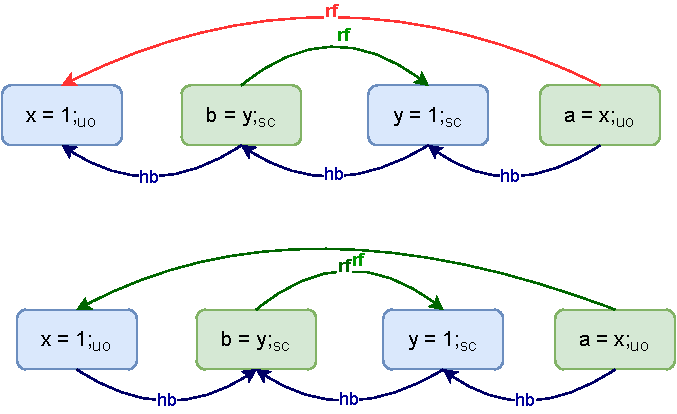
\includegraphics[scale=0.7]{5.InstructionReordering/0.Intro/ReorderingExample2(b).pdf}
            \caption{The set of partial order relations justifying the observable behavior in question for both the candidates in Figure~\ref{reord:example2(a)}.} 
            \label{reord:example2(b)}
        \end{figure}

        The above two examples show that we have to be careful while reordering two events in the same thread. 
        By example analysis, for each observable behavior, one must check all possible candidate executions and assert whether such an observable is possible or not. 
        This method of checking validity of reordering will scale exponentially as the program size increases. 
        It may also be the case that the compiler may not have information on which exact events would be executed in other threads to assert such reordering is valid. 

    
    
    
    
    

%Summary of Approach.
\section{Approach}

    We consider the same set of assumptions for reordering here. 
    Similar to reordering, our main objective is to ensure that the set of possible observable behaviors of a program, remain unchanged after elimination. 
    In the case of write elimination, the property we try to prove remains the same.
    In the case of read elimination though, we would want the observable behaviors excluding the specific read eliminated to be a subset.
    For both cases, if preserving all behaviors is not possible, then we would want the set of observable behaviors after elimination at the very least to be a subset.

    The main difference here is that elimination would remove certain happens-before relations, in contrast to having additional ones.
    From our point of view, we would want only the relations with the eliminated read/write to be removed after the transformation.
    The loss of these relations would certainly not have any new happens-before cycle introduced. 
    However, we still have to check whether the removed relations result in some new behavior. 
    We prove when it does not, by doing case-wise analysis on the type of relations eliminated.  

%Key definitions 
\section{Some Useful Definitions}
Before we go about proving when reordering is valid, we define certain helper definitions for it.

%Something we need to define for sake of proofs
\begin{definition}{Consecutive pair of events (\emph{cons})}
    \label{Cons}
    We define \emph{cons} as a function, which takes two events as input, and gives us a boolean indicating if they are consecutive pairs. Two events $e$ and $d$ are consecutive if they have a direct $\stck{_\textit{ao}}$ relation among them;  i.e those relations that are not derived through transitive property of $\stck{_\textit{hb}}$. 
    \begin{align*}
        (
        e \stck{_\textit{ao}} d  \ \wedge \ 
        \nexists k \ \textit{s.t.} \ 
        e \stck{_\textit{ao}} k  \ \wedge \
        k \stck{_\textit{ao}} d 
        )
        \ \vee \
        (
            d \stck{_\textit{ao}} e  \ \wedge \ 
            \nexists k \ \textit{s.t.} \ 
            d \stck{_\textit{ao}} k  \ \wedge \
            k \stck{_\textit{ao}} e  
        ).
    \end{align*}
\end{definition}

\begin{definition}{Direct happens-before relation (dir)}
    \label{Dir}
    We define \emph{dir} to take an ordered pair of events $(e,d)$ such that $\reln{e}{hb}{d}$ and gives a boolean value to indicate whether this relation is \textit{direct}, which can be formally stated as follows:
    \begin{align*}
        \nexists k \ \text{s.t.} \ \reln{e}{hb}{k} \wedge \reln{k}{hb}{d}.
    \end{align*}
    
    We can infer some useful things using \emph{dir} based on some information on events $e$ and $d$\footnotemark. 
    \begin{enumerate}
        \item If $\et{e}{uo}$, then $dir(e,d) \ \Rightarrow \ cons(e,d).$ 
        \item If $\et{d}{uo}$, then $dir(e,d) \ \Rightarrow \ cons(e,d).$
        \item If $\et{e}{sc}\ \wedge\ e\!\in\!R$, then $dir(e,d) \ \Rightarrow \ cons(e,d).$
        \item If $\et{e}{sc}\ \wedge\ e\!\in\!W$, then $dir(e,d) \ \Rightarrow \ cons(e,d)\ \vee\ \reln{e}{sw}{d}.$
        \item If $\et{d}{sc}\ \wedge\ d\!\in\!W$, then $dir(e,d) \ \Rightarrow \ cons(e,d).$
        \item If $\et{d}{sc}\ \wedge\ e\!\in\!R$, then $dir(e,d) \ \Rightarrow \ cons(e,d)\ \vee\ \reln{e}{sw}{d}.$
    \end{enumerate}

    \footnotetext{They can be proved trivially using definitions of $\stck{_{hb}}, \stck{_{sw}} \text{and} \stck{_{ao}}$}.
\end{definition}


\begin{definition}{Reorderable Pair (Reord)}
    \label{Reord}
    
    We define a boolean function \emph{Reord} that takes two ordered pair of events $(e,d)$ such that $\reln{e}{ao}{d}$ and gives a boolean value indicating if they are a reorderable pair\footnotemark.   
    \begin{align*}
        Reord(e,d) = \\
        (
        &((\et{e}{uo} \ \wedge \ \et{d}{uo}) \ \wedge \ 
                (   
                    (\event{e}{R} \ \wedge \ \event{d}{R}) \ \vee \ 
                    (\Re(e) \cap_\Re \Re(d) = \phi) 
                )
        ) \\ &\vee \\
        &((\et{e}{sc} \ \wedge \ \et{d}{uo}) \ \wedge \ 
                (
                    (\event{e}{W} \ \wedge \ (\Re(e) \cap_\Re \Re(d) = \phi)) 
                )
        ) \\ &\vee \\
        &((\et{e}{uo} \ \wedge \ \et{d}{sc}) \ \wedge \ 
                (
                    (\event{d}{R} \ \wedge \ (\Re(e) \cap_\Re \Re(d) = \phi)) 
                )
        )
        ).
    \end{align*}

    \footnotetext{We later prove that this exact definition defines when a pair of two consecutive events are reorderable.}
\end{definition}



%Key Lemmas 
This chapter addresses the validity of instruction reordering under the ECMAScript memory model.
We first start by showing some examples of Candidate Executions where reordering is not safe in the relaxed memory context.  
We give a brief summary of our approach towards a proof to identify when such a reordering is safe.
Next, we introduce a few more definitions for our purpose, followed by two lemmas that will be instrumental for proofs in this chapter and the next. 
We then formulate a theorem and a corresponding corollary that covers validity of reordering at a Candidate Execution level. 
Lastly, we address reordering at the program level involving conditional branching and loops.
We use counter examples to give a better intuitive understanding of the elements of the proof.
\ \newline
\ \newline  
\hrule 
\ \newline 
\ \newline 


\section{Introduction}
    Instruction reordering is a common transformation done by the compiler/hardware, which is essential to optimizations such as instruction scheduling, loop invariant removal, partial redundancy elimination, etc. 
    However, whether we can do such reordering freely given a concurrent program using relaxed memory accesses is a bit unclear. 
     
    \paragraph{Simple reordering is not straightforward under shared memory semantics}
    The main reason is that memory accesses here, do not just perform the desired operation (i.e Read / Write) but also imply certain visibility guarantees across all the other threads.  
    In our observation, we find that, the relaxed memory model of ECMAScript prescribe semantics for visibility using the $\stck{_{hb}}$ relations. 
    
    \paragraph{Some Examples}
        We show a couple of examples to showcase why reordering may not be that straightforward. 
        Consider the first example in Figure~\ref{reord:example1(a)} below of a Candidate before and after reordering two events.
        The original candidate is to the left and that on the right is after reordering the two reads of $T2$.
        The observable behavior in question is written in the middle(orange box). 
        \begin{figure}[H]
            \centering
            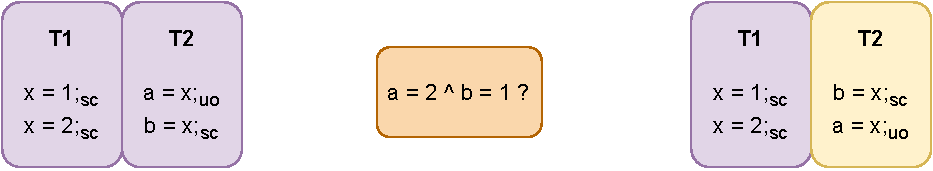
\includegraphics[scale=0.7]{5.InstructionReordering/0.Intro/ReorderingExample1(a).pdf}
            \caption{First example for reordering in candidates of the original program and its reordered counterpart.}
            \label{reord:example1(a)} 
        \end{figure}
        
        Figure~\ref{reord:example1(b)} has two sets of relations. 
        The first justifies the outcome for the reordered Candidate. 
        While the second justifies for the original Candidate. 
        Notice that in the first set of relations, we can infer that one may have a read memory ordered before a write that it reads from. 
        This is quite counter intuitive to understand at first. 
        But strictly from the semantics of the model, this justification to the observable behavior is completely valid\footnotemark. 
        \begin{figure}[H]
            \centering
            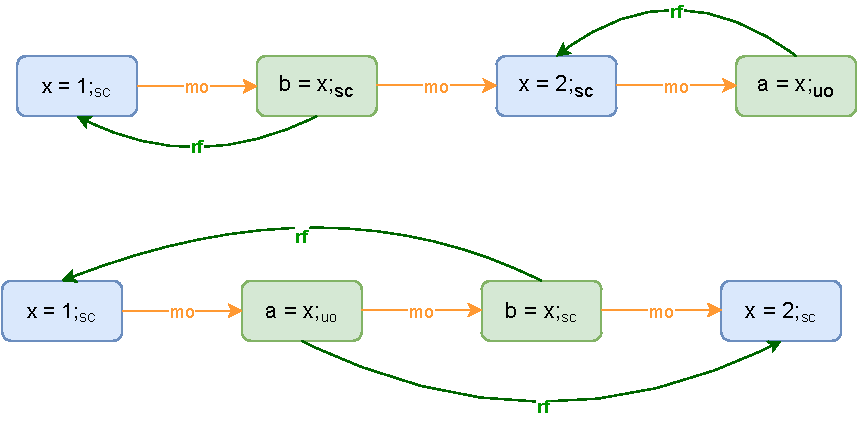
\includegraphics[scale=0.7]{5.InstructionReordering/0.Intro/ReorderingExample1(b).pdf}
            \caption{The set of partial order relations justifying the observable behavior in question for both the candidates in Figure~\ref{reord:example1(a)}.} 
            \label{reord:example1(b)}
        \end{figure}

        \footnotetext{In practice, this can be due to read speculation at the hardware level.}
        
        Consider another example in Figure~\ref{reord:example2(a)}.
        The figure on the left is the original candidate and that on the right is after reordering the two events of $T1$.
        The observable behavior in question is written in the middle(orange box). 
        \begin{figure}[H]
            \centering
            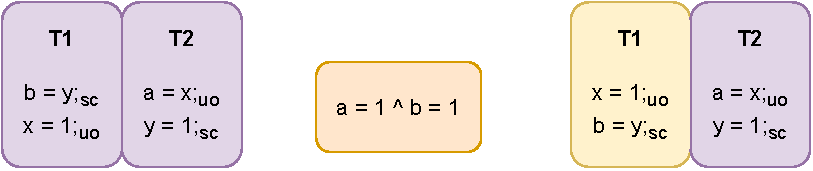
\includegraphics[scale=0.7]{5.InstructionReordering/0.Intro/ReorderingExample2(a).pdf}
            \caption{Second example for reordering with candidates of the original program and its reordered counterpart.} 
            \label{reord:example2(a)}
        \end{figure}
   
        Figure~\ref{reord:example2(b)} has two sets of relations. 
        The first justifies that such an outcome is not possible for the original program candidate due to Axiom \ref{CoRe}. 
        While the second justifies that this outcome is possible for the reordered program.
        Note that we cannot infer in the reordered candidate the set of relations for any candidate execution to have $\reln{a=x;_{uo}}{hb}{x=1;_{uo}}$. 
        \begin{figure}[H]
            \centering
            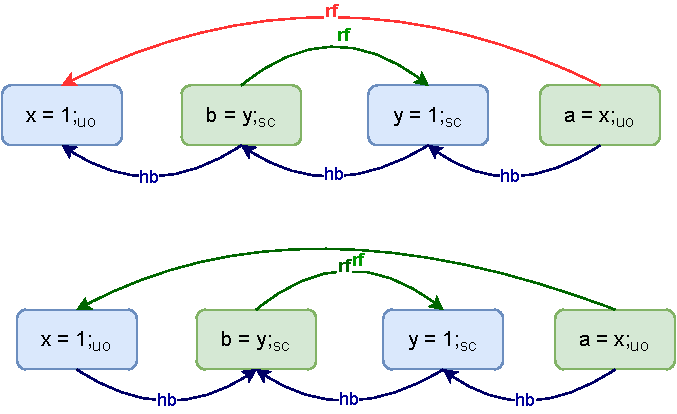
\includegraphics[scale=0.7]{5.InstructionReordering/0.Intro/ReorderingExample2(b).pdf}
            \caption{The set of partial order relations justifying the observable behavior in question for both the candidates in Figure~\ref{reord:example2(a)}.} 
            \label{reord:example2(b)}
        \end{figure}

        The above two examples show that we have to be careful while reordering two events in the same thread. 
        By example analysis, for each observable behavior, one must check all possible candidate executions and assert whether such an observable is possible or not. 
        This method of checking validity of reordering will scale exponentially as the program size increases. 
        It may also be the case that the compiler may not have information on which exact events would be executed in other threads to assert such reordering is valid. 

    
    
    
    
    

%Summary of Approach.
\section{Approach}

    We consider the same set of assumptions for reordering here. 
    Similar to reordering, our main objective is to ensure that the set of possible observable behaviors of a program, remain unchanged after elimination. 
    In the case of write elimination, the property we try to prove remains the same.
    In the case of read elimination though, we would want the observable behaviors excluding the specific read eliminated to be a subset.
    For both cases, if preserving all behaviors is not possible, then we would want the set of observable behaviors after elimination at the very least to be a subset.

    The main difference here is that elimination would remove certain happens-before relations, in contrast to having additional ones.
    From our point of view, we would want only the relations with the eliminated read/write to be removed after the transformation.
    The loss of these relations would certainly not have any new happens-before cycle introduced. 
    However, we still have to check whether the removed relations result in some new behavior. 
    We prove when it does not, by doing case-wise analysis on the type of relations eliminated.  

%Key definitions 
\section{Some Useful Definitions}
Before we go about proving when reordering is valid, we define certain helper definitions for it.

%Something we need to define for sake of proofs
\begin{definition}{Consecutive pair of events (\emph{cons})}
    \label{Cons}
    We define \emph{cons} as a function, which takes two events as input, and gives us a boolean indicating if they are consecutive pairs. Two events $e$ and $d$ are consecutive if they have a direct $\stck{_\textit{ao}}$ relation among them;  i.e those relations that are not derived through transitive property of $\stck{_\textit{hb}}$. 
    \begin{align*}
        (
        e \stck{_\textit{ao}} d  \ \wedge \ 
        \nexists k \ \textit{s.t.} \ 
        e \stck{_\textit{ao}} k  \ \wedge \
        k \stck{_\textit{ao}} d 
        )
        \ \vee \
        (
            d \stck{_\textit{ao}} e  \ \wedge \ 
            \nexists k \ \textit{s.t.} \ 
            d \stck{_\textit{ao}} k  \ \wedge \
            k \stck{_\textit{ao}} e  
        ).
    \end{align*}
\end{definition}

\begin{definition}{Direct happens-before relation (dir)}
    \label{Dir}
    We define \emph{dir} to take an ordered pair of events $(e,d)$ such that $\reln{e}{hb}{d}$ and gives a boolean value to indicate whether this relation is \textit{direct}, which can be formally stated as follows:
    \begin{align*}
        \nexists k \ \text{s.t.} \ \reln{e}{hb}{k} \wedge \reln{k}{hb}{d}.
    \end{align*}
    
    We can infer some useful things using \emph{dir} based on some information on events $e$ and $d$\footnotemark. 
    \begin{enumerate}
        \item If $\et{e}{uo}$, then $dir(e,d) \ \Rightarrow \ cons(e,d).$ 
        \item If $\et{d}{uo}$, then $dir(e,d) \ \Rightarrow \ cons(e,d).$
        \item If $\et{e}{sc}\ \wedge\ e\!\in\!R$, then $dir(e,d) \ \Rightarrow \ cons(e,d).$
        \item If $\et{e}{sc}\ \wedge\ e\!\in\!W$, then $dir(e,d) \ \Rightarrow \ cons(e,d)\ \vee\ \reln{e}{sw}{d}.$
        \item If $\et{d}{sc}\ \wedge\ d\!\in\!W$, then $dir(e,d) \ \Rightarrow \ cons(e,d).$
        \item If $\et{d}{sc}\ \wedge\ e\!\in\!R$, then $dir(e,d) \ \Rightarrow \ cons(e,d)\ \vee\ \reln{e}{sw}{d}.$
    \end{enumerate}

    \footnotetext{They can be proved trivially using definitions of $\stck{_{hb}}, \stck{_{sw}} \text{and} \stck{_{ao}}$}.
\end{definition}


\begin{definition}{Reorderable Pair (Reord)}
    \label{Reord}
    
    We define a boolean function \emph{Reord} that takes two ordered pair of events $(e,d)$ such that $\reln{e}{ao}{d}$ and gives a boolean value indicating if they are a reorderable pair\footnotemark.   
    \begin{align*}
        Reord(e,d) = \\
        (
        &((\et{e}{uo} \ \wedge \ \et{d}{uo}) \ \wedge \ 
                (   
                    (\event{e}{R} \ \wedge \ \event{d}{R}) \ \vee \ 
                    (\Re(e) \cap_\Re \Re(d) = \phi) 
                )
        ) \\ &\vee \\
        &((\et{e}{sc} \ \wedge \ \et{d}{uo}) \ \wedge \ 
                (
                    (\event{e}{W} \ \wedge \ (\Re(e) \cap_\Re \Re(d) = \phi)) 
                )
        ) \\ &\vee \\
        &((\et{e}{uo} \ \wedge \ \et{d}{sc}) \ \wedge \ 
                (
                    (\event{d}{R} \ \wedge \ (\Re(e) \cap_\Re \Re(d) = \phi)) 
                )
        )
        ).
    \end{align*}

    \footnotetext{We later prove that this exact definition defines when a pair of two consecutive events are reorderable.}
\end{definition}



%Key Lemmas 
This chapter addresses the validity of instruction reordering under the ECMAScript memory model.
We first start by showing some examples of Candidate Executions where reordering is not safe in the relaxed memory context.  
We give a brief summary of our approach towards a proof to identify when such a reordering is safe.
Next, we introduce a few more definitions for our purpose, followed by two lemmas that will be instrumental for proofs in this chapter and the next. 
We then formulate a theorem and a corresponding corollary that covers validity of reordering at a Candidate Execution level. 
Lastly, we address reordering at the program level involving conditional branching and loops.
We use counter examples to give a better intuitive understanding of the elements of the proof.
\ \newline
\ \newline  
\hrule 
\ \newline 
\ \newline 


\section{Introduction}
    Instruction reordering is a common transformation done by the compiler/hardware, which is essential to optimizations such as instruction scheduling, loop invariant removal, partial redundancy elimination, etc. 
    However, whether we can do such reordering freely given a concurrent program using relaxed memory accesses is a bit unclear. 
     
    \paragraph{Simple reordering is not straightforward under shared memory semantics}
    The main reason is that memory accesses here, do not just perform the desired operation (i.e Read / Write) but also imply certain visibility guarantees across all the other threads.  
    In our observation, we find that, the relaxed memory model of ECMAScript prescribe semantics for visibility using the $\stck{_{hb}}$ relations. 
    
    \paragraph{Some Examples}
        We show a couple of examples to showcase why reordering may not be that straightforward. 
        Consider the first example in Figure~\ref{reord:example1(a)} below of a Candidate before and after reordering two events.
        The original candidate is to the left and that on the right is after reordering the two reads of $T2$.
        The observable behavior in question is written in the middle(orange box). 
        \begin{figure}[H]
            \centering
            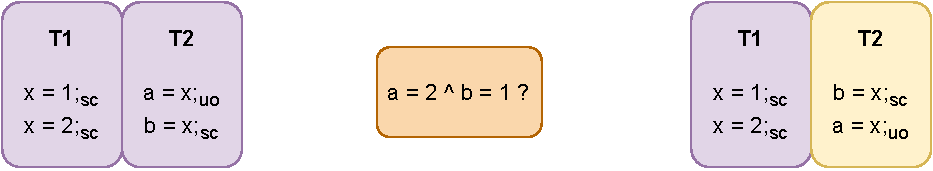
\includegraphics[scale=0.7]{5.InstructionReordering/0.Intro/ReorderingExample1(a).pdf}
            \caption{First example for reordering in candidates of the original program and its reordered counterpart.}
            \label{reord:example1(a)} 
        \end{figure}
        
        Figure~\ref{reord:example1(b)} has two sets of relations. 
        The first justifies the outcome for the reordered Candidate. 
        While the second justifies for the original Candidate. 
        Notice that in the first set of relations, we can infer that one may have a read memory ordered before a write that it reads from. 
        This is quite counter intuitive to understand at first. 
        But strictly from the semantics of the model, this justification to the observable behavior is completely valid\footnotemark. 
        \begin{figure}[H]
            \centering
            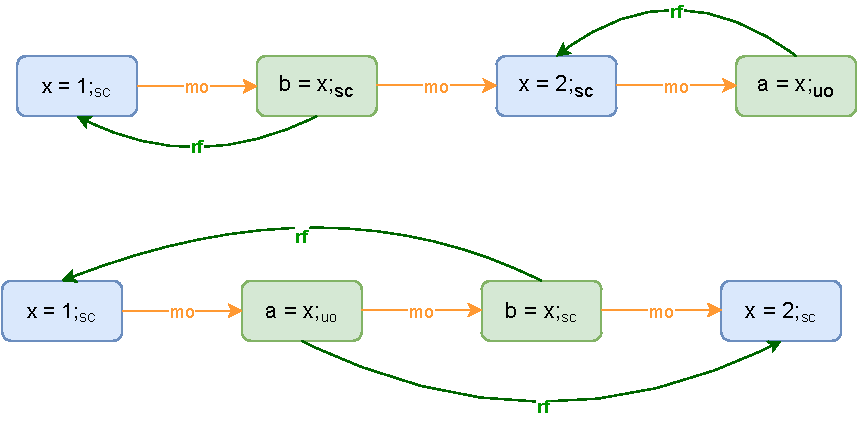
\includegraphics[scale=0.7]{5.InstructionReordering/0.Intro/ReorderingExample1(b).pdf}
            \caption{The set of partial order relations justifying the observable behavior in question for both the candidates in Figure~\ref{reord:example1(a)}.} 
            \label{reord:example1(b)}
        \end{figure}

        \footnotetext{In practice, this can be due to read speculation at the hardware level.}
        
        Consider another example in Figure~\ref{reord:example2(a)}.
        The figure on the left is the original candidate and that on the right is after reordering the two events of $T1$.
        The observable behavior in question is written in the middle(orange box). 
        \begin{figure}[H]
            \centering
            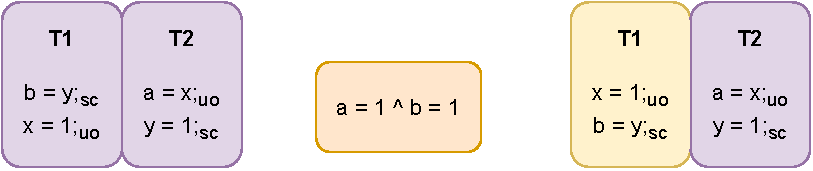
\includegraphics[scale=0.7]{5.InstructionReordering/0.Intro/ReorderingExample2(a).pdf}
            \caption{Second example for reordering with candidates of the original program and its reordered counterpart.} 
            \label{reord:example2(a)}
        \end{figure}
   
        Figure~\ref{reord:example2(b)} has two sets of relations. 
        The first justifies that such an outcome is not possible for the original program candidate due to Axiom \ref{CoRe}. 
        While the second justifies that this outcome is possible for the reordered program.
        Note that we cannot infer in the reordered candidate the set of relations for any candidate execution to have $\reln{a=x;_{uo}}{hb}{x=1;_{uo}}$. 
        \begin{figure}[H]
            \centering
            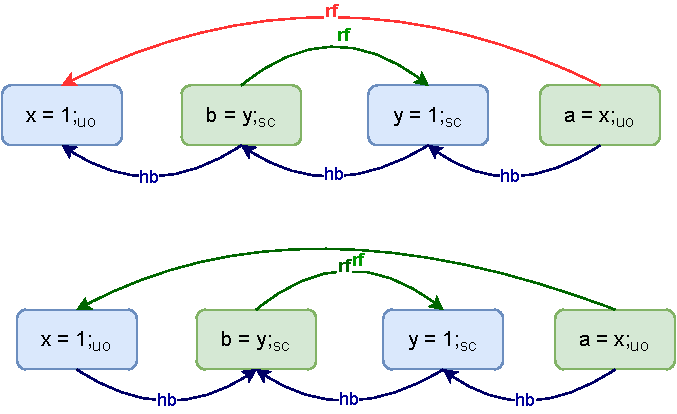
\includegraphics[scale=0.7]{5.InstructionReordering/0.Intro/ReorderingExample2(b).pdf}
            \caption{The set of partial order relations justifying the observable behavior in question for both the candidates in Figure~\ref{reord:example2(a)}.} 
            \label{reord:example2(b)}
        \end{figure}

        The above two examples show that we have to be careful while reordering two events in the same thread. 
        By example analysis, for each observable behavior, one must check all possible candidate executions and assert whether such an observable is possible or not. 
        This method of checking validity of reordering will scale exponentially as the program size increases. 
        It may also be the case that the compiler may not have information on which exact events would be executed in other threads to assert such reordering is valid. 

    
    
    
    
    

%Summary of Approach.
\section{Approach}

    We consider the same set of assumptions for reordering here. 
    Similar to reordering, our main objective is to ensure that the set of possible observable behaviors of a program, remain unchanged after elimination. 
    In the case of write elimination, the property we try to prove remains the same.
    In the case of read elimination though, we would want the observable behaviors excluding the specific read eliminated to be a subset.
    For both cases, if preserving all behaviors is not possible, then we would want the set of observable behaviors after elimination at the very least to be a subset.

    The main difference here is that elimination would remove certain happens-before relations, in contrast to having additional ones.
    From our point of view, we would want only the relations with the eliminated read/write to be removed after the transformation.
    The loss of these relations would certainly not have any new happens-before cycle introduced. 
    However, we still have to check whether the removed relations result in some new behavior. 
    We prove when it does not, by doing case-wise analysis on the type of relations eliminated.  

%Key definitions 
\section{Some Useful Definitions}
Before we go about proving when reordering is valid, we define certain helper definitions for it.

%Something we need to define for sake of proofs
\begin{definition}{Consecutive pair of events (\emph{cons})}
    \label{Cons}
    We define \emph{cons} as a function, which takes two events as input, and gives us a boolean indicating if they are consecutive pairs. Two events $e$ and $d$ are consecutive if they have a direct $\stck{_\textit{ao}}$ relation among them;  i.e those relations that are not derived through transitive property of $\stck{_\textit{hb}}$. 
    \begin{align*}
        (
        e \stck{_\textit{ao}} d  \ \wedge \ 
        \nexists k \ \textit{s.t.} \ 
        e \stck{_\textit{ao}} k  \ \wedge \
        k \stck{_\textit{ao}} d 
        )
        \ \vee \
        (
            d \stck{_\textit{ao}} e  \ \wedge \ 
            \nexists k \ \textit{s.t.} \ 
            d \stck{_\textit{ao}} k  \ \wedge \
            k \stck{_\textit{ao}} e  
        ).
    \end{align*}
\end{definition}

\begin{definition}{Direct happens-before relation (dir)}
    \label{Dir}
    We define \emph{dir} to take an ordered pair of events $(e,d)$ such that $\reln{e}{hb}{d}$ and gives a boolean value to indicate whether this relation is \textit{direct}, which can be formally stated as follows:
    \begin{align*}
        \nexists k \ \text{s.t.} \ \reln{e}{hb}{k} \wedge \reln{k}{hb}{d}.
    \end{align*}
    
    We can infer some useful things using \emph{dir} based on some information on events $e$ and $d$\footnotemark. 
    \begin{enumerate}
        \item If $\et{e}{uo}$, then $dir(e,d) \ \Rightarrow \ cons(e,d).$ 
        \item If $\et{d}{uo}$, then $dir(e,d) \ \Rightarrow \ cons(e,d).$
        \item If $\et{e}{sc}\ \wedge\ e\!\in\!R$, then $dir(e,d) \ \Rightarrow \ cons(e,d).$
        \item If $\et{e}{sc}\ \wedge\ e\!\in\!W$, then $dir(e,d) \ \Rightarrow \ cons(e,d)\ \vee\ \reln{e}{sw}{d}.$
        \item If $\et{d}{sc}\ \wedge\ d\!\in\!W$, then $dir(e,d) \ \Rightarrow \ cons(e,d).$
        \item If $\et{d}{sc}\ \wedge\ e\!\in\!R$, then $dir(e,d) \ \Rightarrow \ cons(e,d)\ \vee\ \reln{e}{sw}{d}.$
    \end{enumerate}

    \footnotetext{They can be proved trivially using definitions of $\stck{_{hb}}, \stck{_{sw}} \text{and} \stck{_{ao}}$}.
\end{definition}


\begin{definition}{Reorderable Pair (Reord)}
    \label{Reord}
    
    We define a boolean function \emph{Reord} that takes two ordered pair of events $(e,d)$ such that $\reln{e}{ao}{d}$ and gives a boolean value indicating if they are a reorderable pair\footnotemark.   
    \begin{align*}
        Reord(e,d) = \\
        (
        &((\et{e}{uo} \ \wedge \ \et{d}{uo}) \ \wedge \ 
                (   
                    (\event{e}{R} \ \wedge \ \event{d}{R}) \ \vee \ 
                    (\Re(e) \cap_\Re \Re(d) = \phi) 
                )
        ) \\ &\vee \\
        &((\et{e}{sc} \ \wedge \ \et{d}{uo}) \ \wedge \ 
                (
                    (\event{e}{W} \ \wedge \ (\Re(e) \cap_\Re \Re(d) = \phi)) 
                )
        ) \\ &\vee \\
        &((\et{e}{uo} \ \wedge \ \et{d}{sc}) \ \wedge \ 
                (
                    (\event{d}{R} \ \wedge \ (\Re(e) \cap_\Re \Re(d) = \phi)) 
                )
        )
        ).
    \end{align*}

    \footnotetext{We later prove that this exact definition defines when a pair of two consecutive events are reorderable.}
\end{definition}



%Key Lemmas 
This chapter addresses the validity of instruction reordering under the ECMAScript memory model.
We first start by showing some examples of Candidate Executions where reordering is not safe in the relaxed memory context.  
We give a brief summary of our approach towards a proof to identify when such a reordering is safe.
Next, we introduce a few more definitions for our purpose, followed by two lemmas that will be instrumental for proofs in this chapter and the next. 
We then formulate a theorem and a corresponding corollary that covers validity of reordering at a Candidate Execution level. 
Lastly, we address reordering at the program level involving conditional branching and loops.
We use counter examples to give a better intuitive understanding of the elements of the proof.
\ \newline
\ \newline  
\hrule 
\ \newline 
\ \newline 

\input{4.InstructionReordering/0.Intro/intro.tex}

%Summary of Approach.
\input{4.InstructionReordering/1.Approach.tex}

%Key definitions 
\input{4.InstructionReordering/2.Definitions.tex}

%Key Lemmas 
\input{4.InstructionReordering/3.Lemmas/main.tex}

%Valid reordering at the Candidate Execution level
\input{4.InstructionReordering/4.ValidReorderingCandidate/main.tex}

%From Candidates to Programs
\input{4.InstructionReordering/5.ValidReorderingProgram/main.tex}

%Conclusion (write here itself. No need for a new .tex file)
\ \newline
\ \newline  
\hrule 
\ \newline 
\ \newline 
To summarize, this chapter addressed the validity of instruction reordering under the ECMAScript Memory Model. 
We first built a conservative proof for reordering based on candidate executions.
We later extended it to programs abstracted to the set of shared memory events. 
We discussed throughout the limitation and advantages of our conservative approach. 
We also presented examples throughout this chapter to get a fair intuitive understanding of the ideas behind the proof and the role of the axiomatic model in it.
In the next chapter, we will address the validity of elimination under the ECMAScript Memory Model.

%Valid reordering at the Candidate Execution level
This chapter addresses the validity of instruction reordering under the ECMAScript memory model.
We first start by showing some examples of Candidate Executions where reordering is not safe in the relaxed memory context.  
We give a brief summary of our approach towards a proof to identify when such a reordering is safe.
Next, we introduce a few more definitions for our purpose, followed by two lemmas that will be instrumental for proofs in this chapter and the next. 
We then formulate a theorem and a corresponding corollary that covers validity of reordering at a Candidate Execution level. 
Lastly, we address reordering at the program level involving conditional branching and loops.
We use counter examples to give a better intuitive understanding of the elements of the proof.
\ \newline
\ \newline  
\hrule 
\ \newline 
\ \newline 

\input{4.InstructionReordering/0.Intro/intro.tex}

%Summary of Approach.
\input{4.InstructionReordering/1.Approach.tex}

%Key definitions 
\input{4.InstructionReordering/2.Definitions.tex}

%Key Lemmas 
\input{4.InstructionReordering/3.Lemmas/main.tex}

%Valid reordering at the Candidate Execution level
\input{4.InstructionReordering/4.ValidReorderingCandidate/main.tex}

%From Candidates to Programs
\input{4.InstructionReordering/5.ValidReorderingProgram/main.tex}

%Conclusion (write here itself. No need for a new .tex file)
\ \newline
\ \newline  
\hrule 
\ \newline 
\ \newline 
To summarize, this chapter addressed the validity of instruction reordering under the ECMAScript Memory Model. 
We first built a conservative proof for reordering based on candidate executions.
We later extended it to programs abstracted to the set of shared memory events. 
We discussed throughout the limitation and advantages of our conservative approach. 
We also presented examples throughout this chapter to get a fair intuitive understanding of the ideas behind the proof and the role of the axiomatic model in it.
In the next chapter, we will address the validity of elimination under the ECMAScript Memory Model.

%From Candidates to Programs
This chapter addresses the validity of instruction reordering under the ECMAScript memory model.
We first start by showing some examples of Candidate Executions where reordering is not safe in the relaxed memory context.  
We give a brief summary of our approach towards a proof to identify when such a reordering is safe.
Next, we introduce a few more definitions for our purpose, followed by two lemmas that will be instrumental for proofs in this chapter and the next. 
We then formulate a theorem and a corresponding corollary that covers validity of reordering at a Candidate Execution level. 
Lastly, we address reordering at the program level involving conditional branching and loops.
We use counter examples to give a better intuitive understanding of the elements of the proof.
\ \newline
\ \newline  
\hrule 
\ \newline 
\ \newline 

\input{4.InstructionReordering/0.Intro/intro.tex}

%Summary of Approach.
\input{4.InstructionReordering/1.Approach.tex}

%Key definitions 
\input{4.InstructionReordering/2.Definitions.tex}

%Key Lemmas 
\input{4.InstructionReordering/3.Lemmas/main.tex}

%Valid reordering at the Candidate Execution level
\input{4.InstructionReordering/4.ValidReorderingCandidate/main.tex}

%From Candidates to Programs
\input{4.InstructionReordering/5.ValidReorderingProgram/main.tex}

%Conclusion (write here itself. No need for a new .tex file)
\ \newline
\ \newline  
\hrule 
\ \newline 
\ \newline 
To summarize, this chapter addressed the validity of instruction reordering under the ECMAScript Memory Model. 
We first built a conservative proof for reordering based on candidate executions.
We later extended it to programs abstracted to the set of shared memory events. 
We discussed throughout the limitation and advantages of our conservative approach. 
We also presented examples throughout this chapter to get a fair intuitive understanding of the ideas behind the proof and the role of the axiomatic model in it.
In the next chapter, we will address the validity of elimination under the ECMAScript Memory Model.

%Conclusion (write here itself. No need for a new .tex file)
\ \newline
\ \newline  
\hrule 
\ \newline 
\ \newline 
To summarize, this chapter addressed the validity of instruction reordering under the ECMAScript Memory Model. 
We first built a conservative proof for reordering based on candidate executions.
We later extended it to programs abstracted to the set of shared memory events. 
We discussed throughout the limitation and advantages of our conservative approach. 
We also presented examples throughout this chapter to get a fair intuitive understanding of the ideas behind the proof and the role of the axiomatic model in it.
In the next chapter, we will address the validity of elimination under the ECMAScript Memory Model.

%Valid reordering at the Candidate Execution level
This chapter addresses the validity of instruction reordering under the ECMAScript memory model.
We first start by showing some examples of Candidate Executions where reordering is not safe in the relaxed memory context.  
We give a brief summary of our approach towards a proof to identify when such a reordering is safe.
Next, we introduce a few more definitions for our purpose, followed by two lemmas that will be instrumental for proofs in this chapter and the next. 
We then formulate a theorem and a corresponding corollary that covers validity of reordering at a Candidate Execution level. 
Lastly, we address reordering at the program level involving conditional branching and loops.
We use counter examples to give a better intuitive understanding of the elements of the proof.
\ \newline
\ \newline  
\hrule 
\ \newline 
\ \newline 


\section{Introduction}
    Instruction reordering is a common transformation done by the compiler/hardware, which is essential to optimizations such as instruction scheduling, loop invariant removal, partial redundancy elimination, etc. 
    However, whether we can do such reordering freely given a concurrent program using relaxed memory accesses is a bit unclear. 
     
    \paragraph{Simple reordering is not straightforward under shared memory semantics}
    The main reason is that memory accesses here, do not just perform the desired operation (i.e Read / Write) but also imply certain visibility guarantees across all the other threads.  
    In our observation, we find that, the relaxed memory model of ECMAScript prescribe semantics for visibility using the $\stck{_{hb}}$ relations. 
    
    \paragraph{Some Examples}
        We show a couple of examples to showcase why reordering may not be that straightforward. 
        Consider the first example in Figure~\ref{reord:example1(a)} below of a Candidate before and after reordering two events.
        The original candidate is to the left and that on the right is after reordering the two reads of $T2$.
        The observable behavior in question is written in the middle(orange box). 
        \begin{figure}[H]
            \centering
            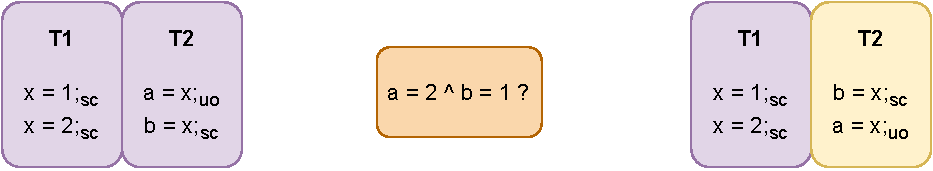
\includegraphics[scale=0.7]{5.InstructionReordering/0.Intro/ReorderingExample1(a).pdf}
            \caption{First example for reordering in candidates of the original program and its reordered counterpart.}
            \label{reord:example1(a)} 
        \end{figure}
        
        Figure~\ref{reord:example1(b)} has two sets of relations. 
        The first justifies the outcome for the reordered Candidate. 
        While the second justifies for the original Candidate. 
        Notice that in the first set of relations, we can infer that one may have a read memory ordered before a write that it reads from. 
        This is quite counter intuitive to understand at first. 
        But strictly from the semantics of the model, this justification to the observable behavior is completely valid\footnotemark. 
        \begin{figure}[H]
            \centering
            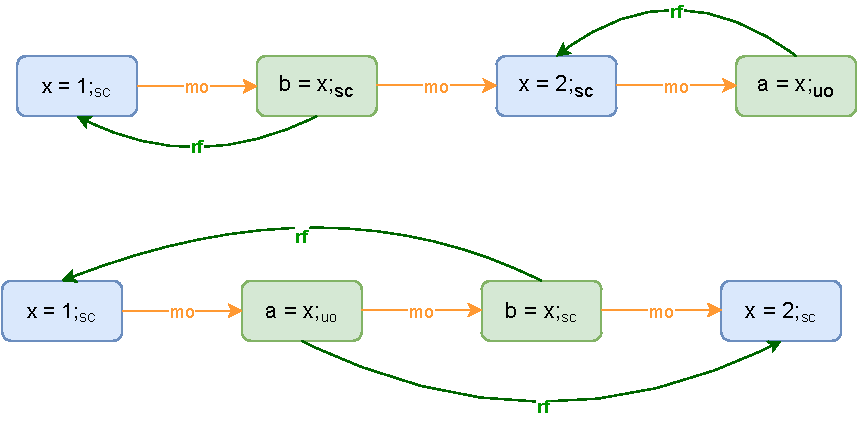
\includegraphics[scale=0.7]{5.InstructionReordering/0.Intro/ReorderingExample1(b).pdf}
            \caption{The set of partial order relations justifying the observable behavior in question for both the candidates in Figure~\ref{reord:example1(a)}.} 
            \label{reord:example1(b)}
        \end{figure}

        \footnotetext{In practice, this can be due to read speculation at the hardware level.}
        
        Consider another example in Figure~\ref{reord:example2(a)}.
        The figure on the left is the original candidate and that on the right is after reordering the two events of $T1$.
        The observable behavior in question is written in the middle(orange box). 
        \begin{figure}[H]
            \centering
            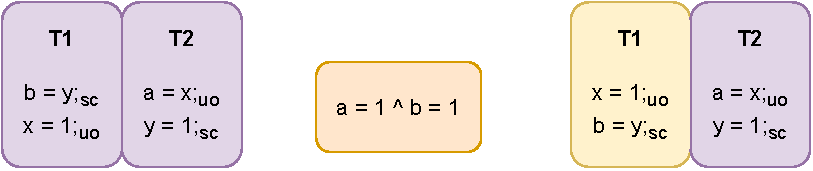
\includegraphics[scale=0.7]{5.InstructionReordering/0.Intro/ReorderingExample2(a).pdf}
            \caption{Second example for reordering with candidates of the original program and its reordered counterpart.} 
            \label{reord:example2(a)}
        \end{figure}
   
        Figure~\ref{reord:example2(b)} has two sets of relations. 
        The first justifies that such an outcome is not possible for the original program candidate due to Axiom \ref{CoRe}. 
        While the second justifies that this outcome is possible for the reordered program.
        Note that we cannot infer in the reordered candidate the set of relations for any candidate execution to have $\reln{a=x;_{uo}}{hb}{x=1;_{uo}}$. 
        \begin{figure}[H]
            \centering
            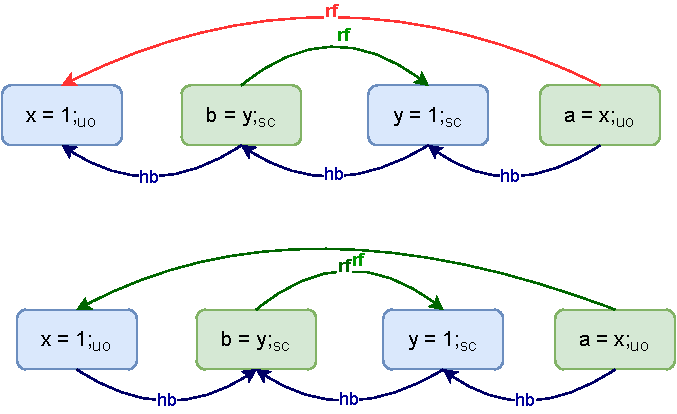
\includegraphics[scale=0.7]{5.InstructionReordering/0.Intro/ReorderingExample2(b).pdf}
            \caption{The set of partial order relations justifying the observable behavior in question for both the candidates in Figure~\ref{reord:example2(a)}.} 
            \label{reord:example2(b)}
        \end{figure}

        The above two examples show that we have to be careful while reordering two events in the same thread. 
        By example analysis, for each observable behavior, one must check all possible candidate executions and assert whether such an observable is possible or not. 
        This method of checking validity of reordering will scale exponentially as the program size increases. 
        It may also be the case that the compiler may not have information on which exact events would be executed in other threads to assert such reordering is valid. 

    
    
    
    
    

%Summary of Approach.
\section{Approach}

    We consider the same set of assumptions for reordering here. 
    Similar to reordering, our main objective is to ensure that the set of possible observable behaviors of a program, remain unchanged after elimination. 
    In the case of write elimination, the property we try to prove remains the same.
    In the case of read elimination though, we would want the observable behaviors excluding the specific read eliminated to be a subset.
    For both cases, if preserving all behaviors is not possible, then we would want the set of observable behaviors after elimination at the very least to be a subset.

    The main difference here is that elimination would remove certain happens-before relations, in contrast to having additional ones.
    From our point of view, we would want only the relations with the eliminated read/write to be removed after the transformation.
    The loss of these relations would certainly not have any new happens-before cycle introduced. 
    However, we still have to check whether the removed relations result in some new behavior. 
    We prove when it does not, by doing case-wise analysis on the type of relations eliminated.  

%Key definitions 
\section{Some Useful Definitions}
Before we go about proving when reordering is valid, we define certain helper definitions for it.

%Something we need to define for sake of proofs
\begin{definition}{Consecutive pair of events (\emph{cons})}
    \label{Cons}
    We define \emph{cons} as a function, which takes two events as input, and gives us a boolean indicating if they are consecutive pairs. Two events $e$ and $d$ are consecutive if they have a direct $\stck{_\textit{ao}}$ relation among them;  i.e those relations that are not derived through transitive property of $\stck{_\textit{hb}}$. 
    \begin{align*}
        (
        e \stck{_\textit{ao}} d  \ \wedge \ 
        \nexists k \ \textit{s.t.} \ 
        e \stck{_\textit{ao}} k  \ \wedge \
        k \stck{_\textit{ao}} d 
        )
        \ \vee \
        (
            d \stck{_\textit{ao}} e  \ \wedge \ 
            \nexists k \ \textit{s.t.} \ 
            d \stck{_\textit{ao}} k  \ \wedge \
            k \stck{_\textit{ao}} e  
        ).
    \end{align*}
\end{definition}

\begin{definition}{Direct happens-before relation (dir)}
    \label{Dir}
    We define \emph{dir} to take an ordered pair of events $(e,d)$ such that $\reln{e}{hb}{d}$ and gives a boolean value to indicate whether this relation is \textit{direct}, which can be formally stated as follows:
    \begin{align*}
        \nexists k \ \text{s.t.} \ \reln{e}{hb}{k} \wedge \reln{k}{hb}{d}.
    \end{align*}
    
    We can infer some useful things using \emph{dir} based on some information on events $e$ and $d$\footnotemark. 
    \begin{enumerate}
        \item If $\et{e}{uo}$, then $dir(e,d) \ \Rightarrow \ cons(e,d).$ 
        \item If $\et{d}{uo}$, then $dir(e,d) \ \Rightarrow \ cons(e,d).$
        \item If $\et{e}{sc}\ \wedge\ e\!\in\!R$, then $dir(e,d) \ \Rightarrow \ cons(e,d).$
        \item If $\et{e}{sc}\ \wedge\ e\!\in\!W$, then $dir(e,d) \ \Rightarrow \ cons(e,d)\ \vee\ \reln{e}{sw}{d}.$
        \item If $\et{d}{sc}\ \wedge\ d\!\in\!W$, then $dir(e,d) \ \Rightarrow \ cons(e,d).$
        \item If $\et{d}{sc}\ \wedge\ e\!\in\!R$, then $dir(e,d) \ \Rightarrow \ cons(e,d)\ \vee\ \reln{e}{sw}{d}.$
    \end{enumerate}

    \footnotetext{They can be proved trivially using definitions of $\stck{_{hb}}, \stck{_{sw}} \text{and} \stck{_{ao}}$}.
\end{definition}


\begin{definition}{Reorderable Pair (Reord)}
    \label{Reord}
    
    We define a boolean function \emph{Reord} that takes two ordered pair of events $(e,d)$ such that $\reln{e}{ao}{d}$ and gives a boolean value indicating if they are a reorderable pair\footnotemark.   
    \begin{align*}
        Reord(e,d) = \\
        (
        &((\et{e}{uo} \ \wedge \ \et{d}{uo}) \ \wedge \ 
                (   
                    (\event{e}{R} \ \wedge \ \event{d}{R}) \ \vee \ 
                    (\Re(e) \cap_\Re \Re(d) = \phi) 
                )
        ) \\ &\vee \\
        &((\et{e}{sc} \ \wedge \ \et{d}{uo}) \ \wedge \ 
                (
                    (\event{e}{W} \ \wedge \ (\Re(e) \cap_\Re \Re(d) = \phi)) 
                )
        ) \\ &\vee \\
        &((\et{e}{uo} \ \wedge \ \et{d}{sc}) \ \wedge \ 
                (
                    (\event{d}{R} \ \wedge \ (\Re(e) \cap_\Re \Re(d) = \phi)) 
                )
        )
        ).
    \end{align*}

    \footnotetext{We later prove that this exact definition defines when a pair of two consecutive events are reorderable.}
\end{definition}



%Key Lemmas 
This chapter addresses the validity of instruction reordering under the ECMAScript memory model.
We first start by showing some examples of Candidate Executions where reordering is not safe in the relaxed memory context.  
We give a brief summary of our approach towards a proof to identify when such a reordering is safe.
Next, we introduce a few more definitions for our purpose, followed by two lemmas that will be instrumental for proofs in this chapter and the next. 
We then formulate a theorem and a corresponding corollary that covers validity of reordering at a Candidate Execution level. 
Lastly, we address reordering at the program level involving conditional branching and loops.
We use counter examples to give a better intuitive understanding of the elements of the proof.
\ \newline
\ \newline  
\hrule 
\ \newline 
\ \newline 

\input{4.InstructionReordering/0.Intro/intro.tex}

%Summary of Approach.
\input{4.InstructionReordering/1.Approach.tex}

%Key definitions 
\input{4.InstructionReordering/2.Definitions.tex}

%Key Lemmas 
\input{4.InstructionReordering/3.Lemmas/main.tex}

%Valid reordering at the Candidate Execution level
\input{4.InstructionReordering/4.ValidReorderingCandidate/main.tex}

%From Candidates to Programs
\input{4.InstructionReordering/5.ValidReorderingProgram/main.tex}

%Conclusion (write here itself. No need for a new .tex file)
\ \newline
\ \newline  
\hrule 
\ \newline 
\ \newline 
To summarize, this chapter addressed the validity of instruction reordering under the ECMAScript Memory Model. 
We first built a conservative proof for reordering based on candidate executions.
We later extended it to programs abstracted to the set of shared memory events. 
We discussed throughout the limitation and advantages of our conservative approach. 
We also presented examples throughout this chapter to get a fair intuitive understanding of the ideas behind the proof and the role of the axiomatic model in it.
In the next chapter, we will address the validity of elimination under the ECMAScript Memory Model.

%Valid reordering at the Candidate Execution level
This chapter addresses the validity of instruction reordering under the ECMAScript memory model.
We first start by showing some examples of Candidate Executions where reordering is not safe in the relaxed memory context.  
We give a brief summary of our approach towards a proof to identify when such a reordering is safe.
Next, we introduce a few more definitions for our purpose, followed by two lemmas that will be instrumental for proofs in this chapter and the next. 
We then formulate a theorem and a corresponding corollary that covers validity of reordering at a Candidate Execution level. 
Lastly, we address reordering at the program level involving conditional branching and loops.
We use counter examples to give a better intuitive understanding of the elements of the proof.
\ \newline
\ \newline  
\hrule 
\ \newline 
\ \newline 

\input{4.InstructionReordering/0.Intro/intro.tex}

%Summary of Approach.
\input{4.InstructionReordering/1.Approach.tex}

%Key definitions 
\input{4.InstructionReordering/2.Definitions.tex}

%Key Lemmas 
\input{4.InstructionReordering/3.Lemmas/main.tex}

%Valid reordering at the Candidate Execution level
\input{4.InstructionReordering/4.ValidReorderingCandidate/main.tex}

%From Candidates to Programs
\input{4.InstructionReordering/5.ValidReorderingProgram/main.tex}

%Conclusion (write here itself. No need for a new .tex file)
\ \newline
\ \newline  
\hrule 
\ \newline 
\ \newline 
To summarize, this chapter addressed the validity of instruction reordering under the ECMAScript Memory Model. 
We first built a conservative proof for reordering based on candidate executions.
We later extended it to programs abstracted to the set of shared memory events. 
We discussed throughout the limitation and advantages of our conservative approach. 
We also presented examples throughout this chapter to get a fair intuitive understanding of the ideas behind the proof and the role of the axiomatic model in it.
In the next chapter, we will address the validity of elimination under the ECMAScript Memory Model.

%From Candidates to Programs
This chapter addresses the validity of instruction reordering under the ECMAScript memory model.
We first start by showing some examples of Candidate Executions where reordering is not safe in the relaxed memory context.  
We give a brief summary of our approach towards a proof to identify when such a reordering is safe.
Next, we introduce a few more definitions for our purpose, followed by two lemmas that will be instrumental for proofs in this chapter and the next. 
We then formulate a theorem and a corresponding corollary that covers validity of reordering at a Candidate Execution level. 
Lastly, we address reordering at the program level involving conditional branching and loops.
We use counter examples to give a better intuitive understanding of the elements of the proof.
\ \newline
\ \newline  
\hrule 
\ \newline 
\ \newline 

\input{4.InstructionReordering/0.Intro/intro.tex}

%Summary of Approach.
\input{4.InstructionReordering/1.Approach.tex}

%Key definitions 
\input{4.InstructionReordering/2.Definitions.tex}

%Key Lemmas 
\input{4.InstructionReordering/3.Lemmas/main.tex}

%Valid reordering at the Candidate Execution level
\input{4.InstructionReordering/4.ValidReorderingCandidate/main.tex}

%From Candidates to Programs
\input{4.InstructionReordering/5.ValidReorderingProgram/main.tex}

%Conclusion (write here itself. No need for a new .tex file)
\ \newline
\ \newline  
\hrule 
\ \newline 
\ \newline 
To summarize, this chapter addressed the validity of instruction reordering under the ECMAScript Memory Model. 
We first built a conservative proof for reordering based on candidate executions.
We later extended it to programs abstracted to the set of shared memory events. 
We discussed throughout the limitation and advantages of our conservative approach. 
We also presented examples throughout this chapter to get a fair intuitive understanding of the ideas behind the proof and the role of the axiomatic model in it.
In the next chapter, we will address the validity of elimination under the ECMAScript Memory Model.

%Conclusion (write here itself. No need for a new .tex file)
\ \newline
\ \newline  
\hrule 
\ \newline 
\ \newline 
To summarize, this chapter addressed the validity of instruction reordering under the ECMAScript Memory Model. 
We first built a conservative proof for reordering based on candidate executions.
We later extended it to programs abstracted to the set of shared memory events. 
We discussed throughout the limitation and advantages of our conservative approach. 
We also presented examples throughout this chapter to get a fair intuitive understanding of the ideas behind the proof and the role of the axiomatic model in it.
In the next chapter, we will address the validity of elimination under the ECMAScript Memory Model.

%From Candidates to Programs
This chapter addresses the validity of instruction reordering under the ECMAScript memory model.
We first start by showing some examples of Candidate Executions where reordering is not safe in the relaxed memory context.  
We give a brief summary of our approach towards a proof to identify when such a reordering is safe.
Next, we introduce a few more definitions for our purpose, followed by two lemmas that will be instrumental for proofs in this chapter and the next. 
We then formulate a theorem and a corresponding corollary that covers validity of reordering at a Candidate Execution level. 
Lastly, we address reordering at the program level involving conditional branching and loops.
We use counter examples to give a better intuitive understanding of the elements of the proof.
\ \newline
\ \newline  
\hrule 
\ \newline 
\ \newline 


\section{Introduction}
    Instruction reordering is a common transformation done by the compiler/hardware, which is essential to optimizations such as instruction scheduling, loop invariant removal, partial redundancy elimination, etc. 
    However, whether we can do such reordering freely given a concurrent program using relaxed memory accesses is a bit unclear. 
     
    \paragraph{Simple reordering is not straightforward under shared memory semantics}
    The main reason is that memory accesses here, do not just perform the desired operation (i.e Read / Write) but also imply certain visibility guarantees across all the other threads.  
    In our observation, we find that, the relaxed memory model of ECMAScript prescribe semantics for visibility using the $\stck{_{hb}}$ relations. 
    
    \paragraph{Some Examples}
        We show a couple of examples to showcase why reordering may not be that straightforward. 
        Consider the first example in Figure~\ref{reord:example1(a)} below of a Candidate before and after reordering two events.
        The original candidate is to the left and that on the right is after reordering the two reads of $T2$.
        The observable behavior in question is written in the middle(orange box). 
        \begin{figure}[H]
            \centering
            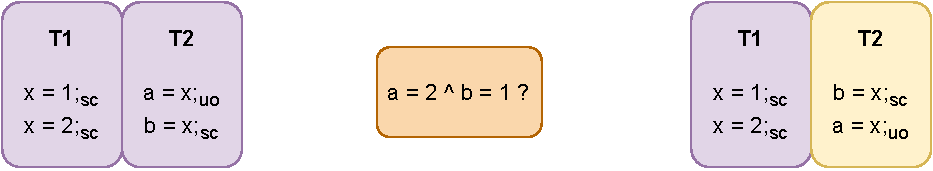
\includegraphics[scale=0.7]{5.InstructionReordering/0.Intro/ReorderingExample1(a).pdf}
            \caption{First example for reordering in candidates of the original program and its reordered counterpart.}
            \label{reord:example1(a)} 
        \end{figure}
        
        Figure~\ref{reord:example1(b)} has two sets of relations. 
        The first justifies the outcome for the reordered Candidate. 
        While the second justifies for the original Candidate. 
        Notice that in the first set of relations, we can infer that one may have a read memory ordered before a write that it reads from. 
        This is quite counter intuitive to understand at first. 
        But strictly from the semantics of the model, this justification to the observable behavior is completely valid\footnotemark. 
        \begin{figure}[H]
            \centering
            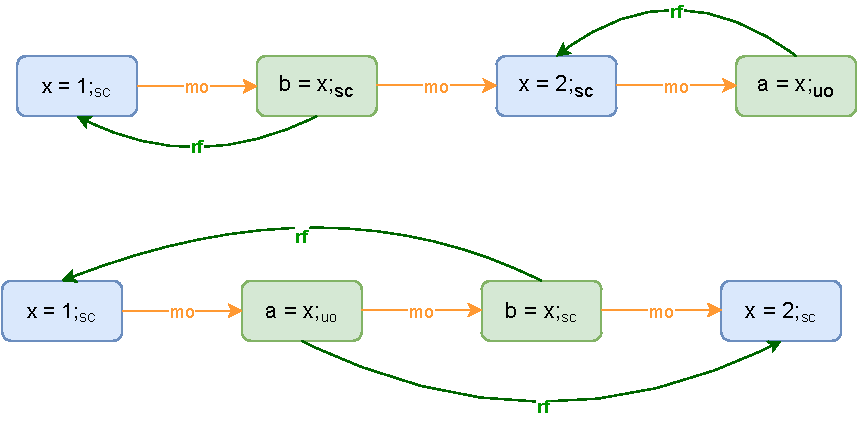
\includegraphics[scale=0.7]{5.InstructionReordering/0.Intro/ReorderingExample1(b).pdf}
            \caption{The set of partial order relations justifying the observable behavior in question for both the candidates in Figure~\ref{reord:example1(a)}.} 
            \label{reord:example1(b)}
        \end{figure}

        \footnotetext{In practice, this can be due to read speculation at the hardware level.}
        
        Consider another example in Figure~\ref{reord:example2(a)}.
        The figure on the left is the original candidate and that on the right is after reordering the two events of $T1$.
        The observable behavior in question is written in the middle(orange box). 
        \begin{figure}[H]
            \centering
            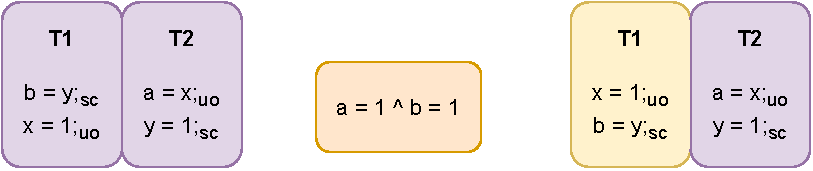
\includegraphics[scale=0.7]{5.InstructionReordering/0.Intro/ReorderingExample2(a).pdf}
            \caption{Second example for reordering with candidates of the original program and its reordered counterpart.} 
            \label{reord:example2(a)}
        \end{figure}
   
        Figure~\ref{reord:example2(b)} has two sets of relations. 
        The first justifies that such an outcome is not possible for the original program candidate due to Axiom \ref{CoRe}. 
        While the second justifies that this outcome is possible for the reordered program.
        Note that we cannot infer in the reordered candidate the set of relations for any candidate execution to have $\reln{a=x;_{uo}}{hb}{x=1;_{uo}}$. 
        \begin{figure}[H]
            \centering
            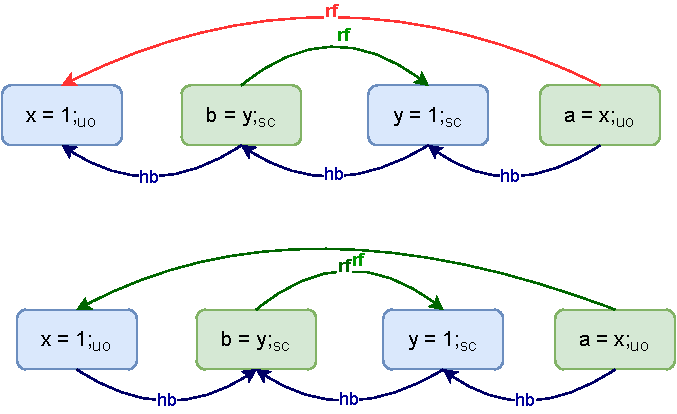
\includegraphics[scale=0.7]{5.InstructionReordering/0.Intro/ReorderingExample2(b).pdf}
            \caption{The set of partial order relations justifying the observable behavior in question for both the candidates in Figure~\ref{reord:example2(a)}.} 
            \label{reord:example2(b)}
        \end{figure}

        The above two examples show that we have to be careful while reordering two events in the same thread. 
        By example analysis, for each observable behavior, one must check all possible candidate executions and assert whether such an observable is possible or not. 
        This method of checking validity of reordering will scale exponentially as the program size increases. 
        It may also be the case that the compiler may not have information on which exact events would be executed in other threads to assert such reordering is valid. 

    
    
    
    
    

%Summary of Approach.
\section{Approach}

    We consider the same set of assumptions for reordering here. 
    Similar to reordering, our main objective is to ensure that the set of possible observable behaviors of a program, remain unchanged after elimination. 
    In the case of write elimination, the property we try to prove remains the same.
    In the case of read elimination though, we would want the observable behaviors excluding the specific read eliminated to be a subset.
    For both cases, if preserving all behaviors is not possible, then we would want the set of observable behaviors after elimination at the very least to be a subset.

    The main difference here is that elimination would remove certain happens-before relations, in contrast to having additional ones.
    From our point of view, we would want only the relations with the eliminated read/write to be removed after the transformation.
    The loss of these relations would certainly not have any new happens-before cycle introduced. 
    However, we still have to check whether the removed relations result in some new behavior. 
    We prove when it does not, by doing case-wise analysis on the type of relations eliminated.  

%Key definitions 
\section{Some Useful Definitions}
Before we go about proving when reordering is valid, we define certain helper definitions for it.

%Something we need to define for sake of proofs
\begin{definition}{Consecutive pair of events (\emph{cons})}
    \label{Cons}
    We define \emph{cons} as a function, which takes two events as input, and gives us a boolean indicating if they are consecutive pairs. Two events $e$ and $d$ are consecutive if they have a direct $\stck{_\textit{ao}}$ relation among them;  i.e those relations that are not derived through transitive property of $\stck{_\textit{hb}}$. 
    \begin{align*}
        (
        e \stck{_\textit{ao}} d  \ \wedge \ 
        \nexists k \ \textit{s.t.} \ 
        e \stck{_\textit{ao}} k  \ \wedge \
        k \stck{_\textit{ao}} d 
        )
        \ \vee \
        (
            d \stck{_\textit{ao}} e  \ \wedge \ 
            \nexists k \ \textit{s.t.} \ 
            d \stck{_\textit{ao}} k  \ \wedge \
            k \stck{_\textit{ao}} e  
        ).
    \end{align*}
\end{definition}

\begin{definition}{Direct happens-before relation (dir)}
    \label{Dir}
    We define \emph{dir} to take an ordered pair of events $(e,d)$ such that $\reln{e}{hb}{d}$ and gives a boolean value to indicate whether this relation is \textit{direct}, which can be formally stated as follows:
    \begin{align*}
        \nexists k \ \text{s.t.} \ \reln{e}{hb}{k} \wedge \reln{k}{hb}{d}.
    \end{align*}
    
    We can infer some useful things using \emph{dir} based on some information on events $e$ and $d$\footnotemark. 
    \begin{enumerate}
        \item If $\et{e}{uo}$, then $dir(e,d) \ \Rightarrow \ cons(e,d).$ 
        \item If $\et{d}{uo}$, then $dir(e,d) \ \Rightarrow \ cons(e,d).$
        \item If $\et{e}{sc}\ \wedge\ e\!\in\!R$, then $dir(e,d) \ \Rightarrow \ cons(e,d).$
        \item If $\et{e}{sc}\ \wedge\ e\!\in\!W$, then $dir(e,d) \ \Rightarrow \ cons(e,d)\ \vee\ \reln{e}{sw}{d}.$
        \item If $\et{d}{sc}\ \wedge\ d\!\in\!W$, then $dir(e,d) \ \Rightarrow \ cons(e,d).$
        \item If $\et{d}{sc}\ \wedge\ e\!\in\!R$, then $dir(e,d) \ \Rightarrow \ cons(e,d)\ \vee\ \reln{e}{sw}{d}.$
    \end{enumerate}

    \footnotetext{They can be proved trivially using definitions of $\stck{_{hb}}, \stck{_{sw}} \text{and} \stck{_{ao}}$}.
\end{definition}


\begin{definition}{Reorderable Pair (Reord)}
    \label{Reord}
    
    We define a boolean function \emph{Reord} that takes two ordered pair of events $(e,d)$ such that $\reln{e}{ao}{d}$ and gives a boolean value indicating if they are a reorderable pair\footnotemark.   
    \begin{align*}
        Reord(e,d) = \\
        (
        &((\et{e}{uo} \ \wedge \ \et{d}{uo}) \ \wedge \ 
                (   
                    (\event{e}{R} \ \wedge \ \event{d}{R}) \ \vee \ 
                    (\Re(e) \cap_\Re \Re(d) = \phi) 
                )
        ) \\ &\vee \\
        &((\et{e}{sc} \ \wedge \ \et{d}{uo}) \ \wedge \ 
                (
                    (\event{e}{W} \ \wedge \ (\Re(e) \cap_\Re \Re(d) = \phi)) 
                )
        ) \\ &\vee \\
        &((\et{e}{uo} \ \wedge \ \et{d}{sc}) \ \wedge \ 
                (
                    (\event{d}{R} \ \wedge \ (\Re(e) \cap_\Re \Re(d) = \phi)) 
                )
        )
        ).
    \end{align*}

    \footnotetext{We later prove that this exact definition defines when a pair of two consecutive events are reorderable.}
\end{definition}



%Key Lemmas 
This chapter addresses the validity of instruction reordering under the ECMAScript memory model.
We first start by showing some examples of Candidate Executions where reordering is not safe in the relaxed memory context.  
We give a brief summary of our approach towards a proof to identify when such a reordering is safe.
Next, we introduce a few more definitions for our purpose, followed by two lemmas that will be instrumental for proofs in this chapter and the next. 
We then formulate a theorem and a corresponding corollary that covers validity of reordering at a Candidate Execution level. 
Lastly, we address reordering at the program level involving conditional branching and loops.
We use counter examples to give a better intuitive understanding of the elements of the proof.
\ \newline
\ \newline  
\hrule 
\ \newline 
\ \newline 

\input{4.InstructionReordering/0.Intro/intro.tex}

%Summary of Approach.
\input{4.InstructionReordering/1.Approach.tex}

%Key definitions 
\input{4.InstructionReordering/2.Definitions.tex}

%Key Lemmas 
\input{4.InstructionReordering/3.Lemmas/main.tex}

%Valid reordering at the Candidate Execution level
\input{4.InstructionReordering/4.ValidReorderingCandidate/main.tex}

%From Candidates to Programs
\input{4.InstructionReordering/5.ValidReorderingProgram/main.tex}

%Conclusion (write here itself. No need for a new .tex file)
\ \newline
\ \newline  
\hrule 
\ \newline 
\ \newline 
To summarize, this chapter addressed the validity of instruction reordering under the ECMAScript Memory Model. 
We first built a conservative proof for reordering based on candidate executions.
We later extended it to programs abstracted to the set of shared memory events. 
We discussed throughout the limitation and advantages of our conservative approach. 
We also presented examples throughout this chapter to get a fair intuitive understanding of the ideas behind the proof and the role of the axiomatic model in it.
In the next chapter, we will address the validity of elimination under the ECMAScript Memory Model.

%Valid reordering at the Candidate Execution level
This chapter addresses the validity of instruction reordering under the ECMAScript memory model.
We first start by showing some examples of Candidate Executions where reordering is not safe in the relaxed memory context.  
We give a brief summary of our approach towards a proof to identify when such a reordering is safe.
Next, we introduce a few more definitions for our purpose, followed by two lemmas that will be instrumental for proofs in this chapter and the next. 
We then formulate a theorem and a corresponding corollary that covers validity of reordering at a Candidate Execution level. 
Lastly, we address reordering at the program level involving conditional branching and loops.
We use counter examples to give a better intuitive understanding of the elements of the proof.
\ \newline
\ \newline  
\hrule 
\ \newline 
\ \newline 

\input{4.InstructionReordering/0.Intro/intro.tex}

%Summary of Approach.
\input{4.InstructionReordering/1.Approach.tex}

%Key definitions 
\input{4.InstructionReordering/2.Definitions.tex}

%Key Lemmas 
\input{4.InstructionReordering/3.Lemmas/main.tex}

%Valid reordering at the Candidate Execution level
\input{4.InstructionReordering/4.ValidReorderingCandidate/main.tex}

%From Candidates to Programs
\input{4.InstructionReordering/5.ValidReorderingProgram/main.tex}

%Conclusion (write here itself. No need for a new .tex file)
\ \newline
\ \newline  
\hrule 
\ \newline 
\ \newline 
To summarize, this chapter addressed the validity of instruction reordering under the ECMAScript Memory Model. 
We first built a conservative proof for reordering based on candidate executions.
We later extended it to programs abstracted to the set of shared memory events. 
We discussed throughout the limitation and advantages of our conservative approach. 
We also presented examples throughout this chapter to get a fair intuitive understanding of the ideas behind the proof and the role of the axiomatic model in it.
In the next chapter, we will address the validity of elimination under the ECMAScript Memory Model.

%From Candidates to Programs
This chapter addresses the validity of instruction reordering under the ECMAScript memory model.
We first start by showing some examples of Candidate Executions where reordering is not safe in the relaxed memory context.  
We give a brief summary of our approach towards a proof to identify when such a reordering is safe.
Next, we introduce a few more definitions for our purpose, followed by two lemmas that will be instrumental for proofs in this chapter and the next. 
We then formulate a theorem and a corresponding corollary that covers validity of reordering at a Candidate Execution level. 
Lastly, we address reordering at the program level involving conditional branching and loops.
We use counter examples to give a better intuitive understanding of the elements of the proof.
\ \newline
\ \newline  
\hrule 
\ \newline 
\ \newline 

\input{4.InstructionReordering/0.Intro/intro.tex}

%Summary of Approach.
\input{4.InstructionReordering/1.Approach.tex}

%Key definitions 
\input{4.InstructionReordering/2.Definitions.tex}

%Key Lemmas 
\input{4.InstructionReordering/3.Lemmas/main.tex}

%Valid reordering at the Candidate Execution level
\input{4.InstructionReordering/4.ValidReorderingCandidate/main.tex}

%From Candidates to Programs
\input{4.InstructionReordering/5.ValidReorderingProgram/main.tex}

%Conclusion (write here itself. No need for a new .tex file)
\ \newline
\ \newline  
\hrule 
\ \newline 
\ \newline 
To summarize, this chapter addressed the validity of instruction reordering under the ECMAScript Memory Model. 
We first built a conservative proof for reordering based on candidate executions.
We later extended it to programs abstracted to the set of shared memory events. 
We discussed throughout the limitation and advantages of our conservative approach. 
We also presented examples throughout this chapter to get a fair intuitive understanding of the ideas behind the proof and the role of the axiomatic model in it.
In the next chapter, we will address the validity of elimination under the ECMAScript Memory Model.

%Conclusion (write here itself. No need for a new .tex file)
\ \newline
\ \newline  
\hrule 
\ \newline 
\ \newline 
To summarize, this chapter addressed the validity of instruction reordering under the ECMAScript Memory Model. 
We first built a conservative proof for reordering based on candidate executions.
We later extended it to programs abstracted to the set of shared memory events. 
We discussed throughout the limitation and advantages of our conservative approach. 
We also presented examples throughout this chapter to get a fair intuitive understanding of the ideas behind the proof and the role of the axiomatic model in it.
In the next chapter, we will address the validity of elimination under the ECMAScript Memory Model.

%Conclusion (write here itself. No need for a new .tex file)
\ \newline
\ \newline  
\hrule 
\ \newline 
\ \newline 
To summarize, this chapter addressed the validity of instruction reordering under the ECMAScript Memory Model. 
We first built a conservative proof for reordering based on candidate executions.
We later extended it to programs abstracted to the set of shared memory events. 
We discussed throughout the limitation and advantages of our conservative approach. 
We also presented examples throughout this chapter to get a fair intuitive understanding of the ideas behind the proof and the role of the axiomatic model in it.
In the next chapter, we will address the validity of elimination under the ECMAScript Memory Model.

%Valid reordering at the Candidate Execution level
This chapter addresses the validity of instruction reordering under the ECMAScript memory model.
We first start by showing some examples of Candidate Executions where reordering is not safe in the relaxed memory context.  
We give a brief summary of our approach towards a proof to identify when such a reordering is safe.
Next, we introduce a few more definitions for our purpose, followed by two lemmas that will be instrumental for proofs in this chapter and the next. 
We then formulate a theorem and a corresponding corollary that covers validity of reordering at a Candidate Execution level. 
Lastly, we address reordering at the program level involving conditional branching and loops.
We use counter examples to give a better intuitive understanding of the elements of the proof.
\ \newline
\ \newline  
\hrule 
\ \newline 
\ \newline 


\section{Introduction}
    Instruction reordering is a common transformation done by the compiler/hardware, which is essential to optimizations such as instruction scheduling, loop invariant removal, partial redundancy elimination, etc. 
    However, whether we can do such reordering freely given a concurrent program using relaxed memory accesses is a bit unclear. 
     
    \paragraph{Simple reordering is not straightforward under shared memory semantics}
    The main reason is that memory accesses here, do not just perform the desired operation (i.e Read / Write) but also imply certain visibility guarantees across all the other threads.  
    In our observation, we find that, the relaxed memory model of ECMAScript prescribe semantics for visibility using the $\stck{_{hb}}$ relations. 
    
    \paragraph{Some Examples}
        We show a couple of examples to showcase why reordering may not be that straightforward. 
        Consider the first example in Figure~\ref{reord:example1(a)} below of a Candidate before and after reordering two events.
        The original candidate is to the left and that on the right is after reordering the two reads of $T2$.
        The observable behavior in question is written in the middle(orange box). 
        \begin{figure}[H]
            \centering
            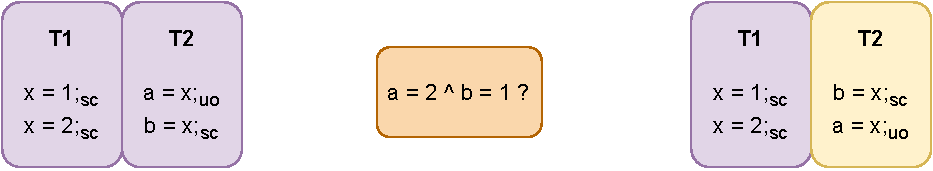
\includegraphics[scale=0.7]{5.InstructionReordering/0.Intro/ReorderingExample1(a).pdf}
            \caption{First example for reordering in candidates of the original program and its reordered counterpart.}
            \label{reord:example1(a)} 
        \end{figure}
        
        Figure~\ref{reord:example1(b)} has two sets of relations. 
        The first justifies the outcome for the reordered Candidate. 
        While the second justifies for the original Candidate. 
        Notice that in the first set of relations, we can infer that one may have a read memory ordered before a write that it reads from. 
        This is quite counter intuitive to understand at first. 
        But strictly from the semantics of the model, this justification to the observable behavior is completely valid\footnotemark. 
        \begin{figure}[H]
            \centering
            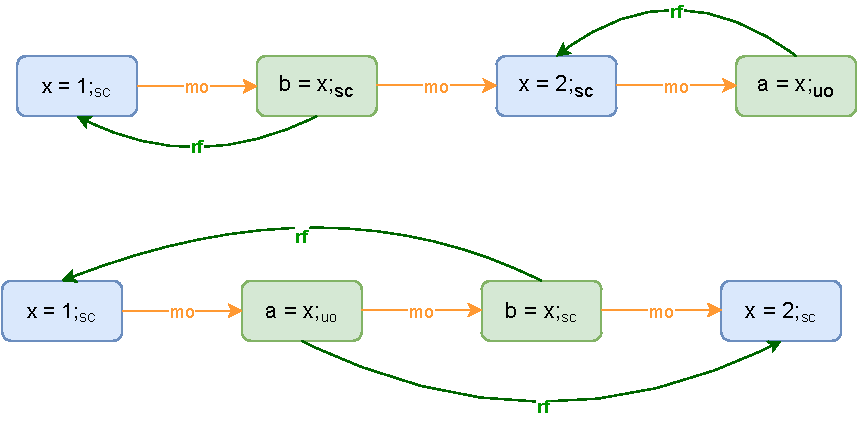
\includegraphics[scale=0.7]{5.InstructionReordering/0.Intro/ReorderingExample1(b).pdf}
            \caption{The set of partial order relations justifying the observable behavior in question for both the candidates in Figure~\ref{reord:example1(a)}.} 
            \label{reord:example1(b)}
        \end{figure}

        \footnotetext{In practice, this can be due to read speculation at the hardware level.}
        
        Consider another example in Figure~\ref{reord:example2(a)}.
        The figure on the left is the original candidate and that on the right is after reordering the two events of $T1$.
        The observable behavior in question is written in the middle(orange box). 
        \begin{figure}[H]
            \centering
            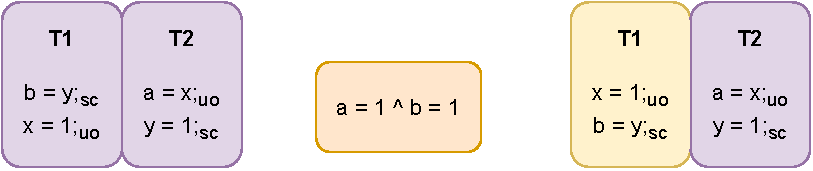
\includegraphics[scale=0.7]{5.InstructionReordering/0.Intro/ReorderingExample2(a).pdf}
            \caption{Second example for reordering with candidates of the original program and its reordered counterpart.} 
            \label{reord:example2(a)}
        \end{figure}
   
        Figure~\ref{reord:example2(b)} has two sets of relations. 
        The first justifies that such an outcome is not possible for the original program candidate due to Axiom \ref{CoRe}. 
        While the second justifies that this outcome is possible for the reordered program.
        Note that we cannot infer in the reordered candidate the set of relations for any candidate execution to have $\reln{a=x;_{uo}}{hb}{x=1;_{uo}}$. 
        \begin{figure}[H]
            \centering
            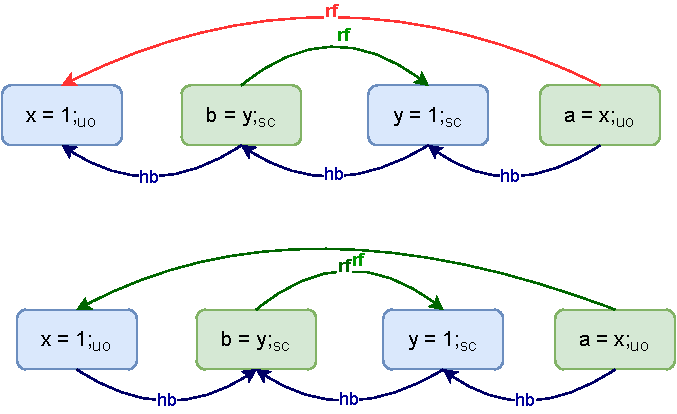
\includegraphics[scale=0.7]{5.InstructionReordering/0.Intro/ReorderingExample2(b).pdf}
            \caption{The set of partial order relations justifying the observable behavior in question for both the candidates in Figure~\ref{reord:example2(a)}.} 
            \label{reord:example2(b)}
        \end{figure}

        The above two examples show that we have to be careful while reordering two events in the same thread. 
        By example analysis, for each observable behavior, one must check all possible candidate executions and assert whether such an observable is possible or not. 
        This method of checking validity of reordering will scale exponentially as the program size increases. 
        It may also be the case that the compiler may not have information on which exact events would be executed in other threads to assert such reordering is valid. 

    
    
    
    
    

%Summary of Approach.
\section{Approach}

    We consider the same set of assumptions for reordering here. 
    Similar to reordering, our main objective is to ensure that the set of possible observable behaviors of a program, remain unchanged after elimination. 
    In the case of write elimination, the property we try to prove remains the same.
    In the case of read elimination though, we would want the observable behaviors excluding the specific read eliminated to be a subset.
    For both cases, if preserving all behaviors is not possible, then we would want the set of observable behaviors after elimination at the very least to be a subset.

    The main difference here is that elimination would remove certain happens-before relations, in contrast to having additional ones.
    From our point of view, we would want only the relations with the eliminated read/write to be removed after the transformation.
    The loss of these relations would certainly not have any new happens-before cycle introduced. 
    However, we still have to check whether the removed relations result in some new behavior. 
    We prove when it does not, by doing case-wise analysis on the type of relations eliminated.  

%Key definitions 
\section{Some Useful Definitions}
Before we go about proving when reordering is valid, we define certain helper definitions for it.

%Something we need to define for sake of proofs
\begin{definition}{Consecutive pair of events (\emph{cons})}
    \label{Cons}
    We define \emph{cons} as a function, which takes two events as input, and gives us a boolean indicating if they are consecutive pairs. Two events $e$ and $d$ are consecutive if they have a direct $\stck{_\textit{ao}}$ relation among them;  i.e those relations that are not derived through transitive property of $\stck{_\textit{hb}}$. 
    \begin{align*}
        (
        e \stck{_\textit{ao}} d  \ \wedge \ 
        \nexists k \ \textit{s.t.} \ 
        e \stck{_\textit{ao}} k  \ \wedge \
        k \stck{_\textit{ao}} d 
        )
        \ \vee \
        (
            d \stck{_\textit{ao}} e  \ \wedge \ 
            \nexists k \ \textit{s.t.} \ 
            d \stck{_\textit{ao}} k  \ \wedge \
            k \stck{_\textit{ao}} e  
        ).
    \end{align*}
\end{definition}

\begin{definition}{Direct happens-before relation (dir)}
    \label{Dir}
    We define \emph{dir} to take an ordered pair of events $(e,d)$ such that $\reln{e}{hb}{d}$ and gives a boolean value to indicate whether this relation is \textit{direct}, which can be formally stated as follows:
    \begin{align*}
        \nexists k \ \text{s.t.} \ \reln{e}{hb}{k} \wedge \reln{k}{hb}{d}.
    \end{align*}
    
    We can infer some useful things using \emph{dir} based on some information on events $e$ and $d$\footnotemark. 
    \begin{enumerate}
        \item If $\et{e}{uo}$, then $dir(e,d) \ \Rightarrow \ cons(e,d).$ 
        \item If $\et{d}{uo}$, then $dir(e,d) \ \Rightarrow \ cons(e,d).$
        \item If $\et{e}{sc}\ \wedge\ e\!\in\!R$, then $dir(e,d) \ \Rightarrow \ cons(e,d).$
        \item If $\et{e}{sc}\ \wedge\ e\!\in\!W$, then $dir(e,d) \ \Rightarrow \ cons(e,d)\ \vee\ \reln{e}{sw}{d}.$
        \item If $\et{d}{sc}\ \wedge\ d\!\in\!W$, then $dir(e,d) \ \Rightarrow \ cons(e,d).$
        \item If $\et{d}{sc}\ \wedge\ e\!\in\!R$, then $dir(e,d) \ \Rightarrow \ cons(e,d)\ \vee\ \reln{e}{sw}{d}.$
    \end{enumerate}

    \footnotetext{They can be proved trivially using definitions of $\stck{_{hb}}, \stck{_{sw}} \text{and} \stck{_{ao}}$}.
\end{definition}


\begin{definition}{Reorderable Pair (Reord)}
    \label{Reord}
    
    We define a boolean function \emph{Reord} that takes two ordered pair of events $(e,d)$ such that $\reln{e}{ao}{d}$ and gives a boolean value indicating if they are a reorderable pair\footnotemark.   
    \begin{align*}
        Reord(e,d) = \\
        (
        &((\et{e}{uo} \ \wedge \ \et{d}{uo}) \ \wedge \ 
                (   
                    (\event{e}{R} \ \wedge \ \event{d}{R}) \ \vee \ 
                    (\Re(e) \cap_\Re \Re(d) = \phi) 
                )
        ) \\ &\vee \\
        &((\et{e}{sc} \ \wedge \ \et{d}{uo}) \ \wedge \ 
                (
                    (\event{e}{W} \ \wedge \ (\Re(e) \cap_\Re \Re(d) = \phi)) 
                )
        ) \\ &\vee \\
        &((\et{e}{uo} \ \wedge \ \et{d}{sc}) \ \wedge \ 
                (
                    (\event{d}{R} \ \wedge \ (\Re(e) \cap_\Re \Re(d) = \phi)) 
                )
        )
        ).
    \end{align*}

    \footnotetext{We later prove that this exact definition defines when a pair of two consecutive events are reorderable.}
\end{definition}



%Key Lemmas 
This chapter addresses the validity of instruction reordering under the ECMAScript memory model.
We first start by showing some examples of Candidate Executions where reordering is not safe in the relaxed memory context.  
We give a brief summary of our approach towards a proof to identify when such a reordering is safe.
Next, we introduce a few more definitions for our purpose, followed by two lemmas that will be instrumental for proofs in this chapter and the next. 
We then formulate a theorem and a corresponding corollary that covers validity of reordering at a Candidate Execution level. 
Lastly, we address reordering at the program level involving conditional branching and loops.
We use counter examples to give a better intuitive understanding of the elements of the proof.
\ \newline
\ \newline  
\hrule 
\ \newline 
\ \newline 


\section{Introduction}
    Instruction reordering is a common transformation done by the compiler/hardware, which is essential to optimizations such as instruction scheduling, loop invariant removal, partial redundancy elimination, etc. 
    However, whether we can do such reordering freely given a concurrent program using relaxed memory accesses is a bit unclear. 
     
    \paragraph{Simple reordering is not straightforward under shared memory semantics}
    The main reason is that memory accesses here, do not just perform the desired operation (i.e Read / Write) but also imply certain visibility guarantees across all the other threads.  
    In our observation, we find that, the relaxed memory model of ECMAScript prescribe semantics for visibility using the $\stck{_{hb}}$ relations. 
    
    \paragraph{Some Examples}
        We show a couple of examples to showcase why reordering may not be that straightforward. 
        Consider the first example in Figure~\ref{reord:example1(a)} below of a Candidate before and after reordering two events.
        The original candidate is to the left and that on the right is after reordering the two reads of $T2$.
        The observable behavior in question is written in the middle(orange box). 
        \begin{figure}[H]
            \centering
            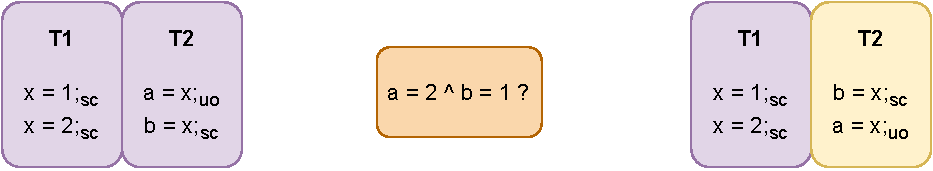
\includegraphics[scale=0.7]{5.InstructionReordering/0.Intro/ReorderingExample1(a).pdf}
            \caption{First example for reordering in candidates of the original program and its reordered counterpart.}
            \label{reord:example1(a)} 
        \end{figure}
        
        Figure~\ref{reord:example1(b)} has two sets of relations. 
        The first justifies the outcome for the reordered Candidate. 
        While the second justifies for the original Candidate. 
        Notice that in the first set of relations, we can infer that one may have a read memory ordered before a write that it reads from. 
        This is quite counter intuitive to understand at first. 
        But strictly from the semantics of the model, this justification to the observable behavior is completely valid\footnotemark. 
        \begin{figure}[H]
            \centering
            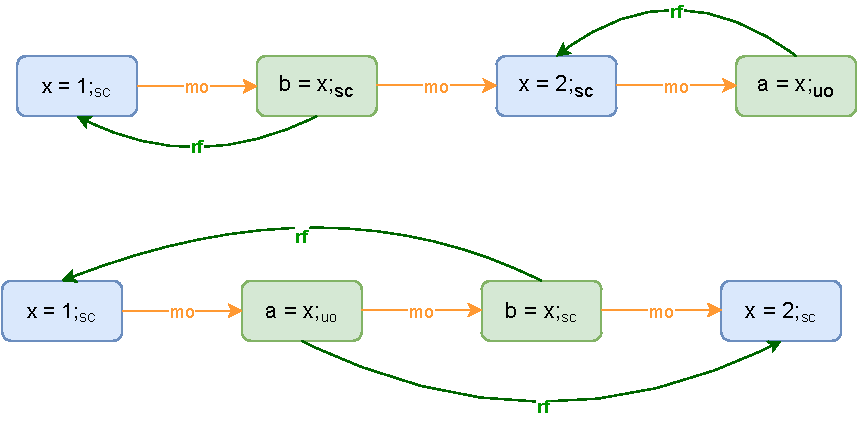
\includegraphics[scale=0.7]{5.InstructionReordering/0.Intro/ReorderingExample1(b).pdf}
            \caption{The set of partial order relations justifying the observable behavior in question for both the candidates in Figure~\ref{reord:example1(a)}.} 
            \label{reord:example1(b)}
        \end{figure}

        \footnotetext{In practice, this can be due to read speculation at the hardware level.}
        
        Consider another example in Figure~\ref{reord:example2(a)}.
        The figure on the left is the original candidate and that on the right is after reordering the two events of $T1$.
        The observable behavior in question is written in the middle(orange box). 
        \begin{figure}[H]
            \centering
            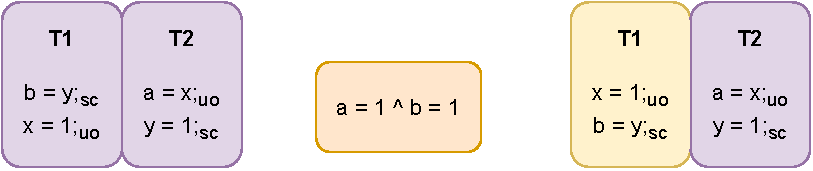
\includegraphics[scale=0.7]{5.InstructionReordering/0.Intro/ReorderingExample2(a).pdf}
            \caption{Second example for reordering with candidates of the original program and its reordered counterpart.} 
            \label{reord:example2(a)}
        \end{figure}
   
        Figure~\ref{reord:example2(b)} has two sets of relations. 
        The first justifies that such an outcome is not possible for the original program candidate due to Axiom \ref{CoRe}. 
        While the second justifies that this outcome is possible for the reordered program.
        Note that we cannot infer in the reordered candidate the set of relations for any candidate execution to have $\reln{a=x;_{uo}}{hb}{x=1;_{uo}}$. 
        \begin{figure}[H]
            \centering
            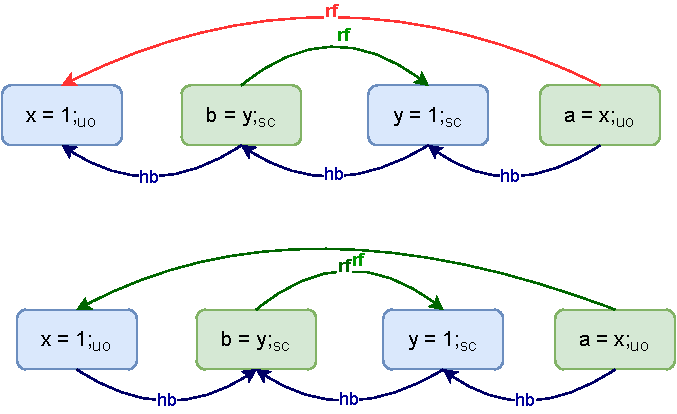
\includegraphics[scale=0.7]{5.InstructionReordering/0.Intro/ReorderingExample2(b).pdf}
            \caption{The set of partial order relations justifying the observable behavior in question for both the candidates in Figure~\ref{reord:example2(a)}.} 
            \label{reord:example2(b)}
        \end{figure}

        The above two examples show that we have to be careful while reordering two events in the same thread. 
        By example analysis, for each observable behavior, one must check all possible candidate executions and assert whether such an observable is possible or not. 
        This method of checking validity of reordering will scale exponentially as the program size increases. 
        It may also be the case that the compiler may not have information on which exact events would be executed in other threads to assert such reordering is valid. 

    
    
    
    
    

%Summary of Approach.
\section{Approach}

    We consider the same set of assumptions for reordering here. 
    Similar to reordering, our main objective is to ensure that the set of possible observable behaviors of a program, remain unchanged after elimination. 
    In the case of write elimination, the property we try to prove remains the same.
    In the case of read elimination though, we would want the observable behaviors excluding the specific read eliminated to be a subset.
    For both cases, if preserving all behaviors is not possible, then we would want the set of observable behaviors after elimination at the very least to be a subset.

    The main difference here is that elimination would remove certain happens-before relations, in contrast to having additional ones.
    From our point of view, we would want only the relations with the eliminated read/write to be removed after the transformation.
    The loss of these relations would certainly not have any new happens-before cycle introduced. 
    However, we still have to check whether the removed relations result in some new behavior. 
    We prove when it does not, by doing case-wise analysis on the type of relations eliminated.  

%Key definitions 
\section{Some Useful Definitions}
Before we go about proving when reordering is valid, we define certain helper definitions for it.

%Something we need to define for sake of proofs
\begin{definition}{Consecutive pair of events (\emph{cons})}
    \label{Cons}
    We define \emph{cons} as a function, which takes two events as input, and gives us a boolean indicating if they are consecutive pairs. Two events $e$ and $d$ are consecutive if they have a direct $\stck{_\textit{ao}}$ relation among them;  i.e those relations that are not derived through transitive property of $\stck{_\textit{hb}}$. 
    \begin{align*}
        (
        e \stck{_\textit{ao}} d  \ \wedge \ 
        \nexists k \ \textit{s.t.} \ 
        e \stck{_\textit{ao}} k  \ \wedge \
        k \stck{_\textit{ao}} d 
        )
        \ \vee \
        (
            d \stck{_\textit{ao}} e  \ \wedge \ 
            \nexists k \ \textit{s.t.} \ 
            d \stck{_\textit{ao}} k  \ \wedge \
            k \stck{_\textit{ao}} e  
        ).
    \end{align*}
\end{definition}

\begin{definition}{Direct happens-before relation (dir)}
    \label{Dir}
    We define \emph{dir} to take an ordered pair of events $(e,d)$ such that $\reln{e}{hb}{d}$ and gives a boolean value to indicate whether this relation is \textit{direct}, which can be formally stated as follows:
    \begin{align*}
        \nexists k \ \text{s.t.} \ \reln{e}{hb}{k} \wedge \reln{k}{hb}{d}.
    \end{align*}
    
    We can infer some useful things using \emph{dir} based on some information on events $e$ and $d$\footnotemark. 
    \begin{enumerate}
        \item If $\et{e}{uo}$, then $dir(e,d) \ \Rightarrow \ cons(e,d).$ 
        \item If $\et{d}{uo}$, then $dir(e,d) \ \Rightarrow \ cons(e,d).$
        \item If $\et{e}{sc}\ \wedge\ e\!\in\!R$, then $dir(e,d) \ \Rightarrow \ cons(e,d).$
        \item If $\et{e}{sc}\ \wedge\ e\!\in\!W$, then $dir(e,d) \ \Rightarrow \ cons(e,d)\ \vee\ \reln{e}{sw}{d}.$
        \item If $\et{d}{sc}\ \wedge\ d\!\in\!W$, then $dir(e,d) \ \Rightarrow \ cons(e,d).$
        \item If $\et{d}{sc}\ \wedge\ e\!\in\!R$, then $dir(e,d) \ \Rightarrow \ cons(e,d)\ \vee\ \reln{e}{sw}{d}.$
    \end{enumerate}

    \footnotetext{They can be proved trivially using definitions of $\stck{_{hb}}, \stck{_{sw}} \text{and} \stck{_{ao}}$}.
\end{definition}


\begin{definition}{Reorderable Pair (Reord)}
    \label{Reord}
    
    We define a boolean function \emph{Reord} that takes two ordered pair of events $(e,d)$ such that $\reln{e}{ao}{d}$ and gives a boolean value indicating if they are a reorderable pair\footnotemark.   
    \begin{align*}
        Reord(e,d) = \\
        (
        &((\et{e}{uo} \ \wedge \ \et{d}{uo}) \ \wedge \ 
                (   
                    (\event{e}{R} \ \wedge \ \event{d}{R}) \ \vee \ 
                    (\Re(e) \cap_\Re \Re(d) = \phi) 
                )
        ) \\ &\vee \\
        &((\et{e}{sc} \ \wedge \ \et{d}{uo}) \ \wedge \ 
                (
                    (\event{e}{W} \ \wedge \ (\Re(e) \cap_\Re \Re(d) = \phi)) 
                )
        ) \\ &\vee \\
        &((\et{e}{uo} \ \wedge \ \et{d}{sc}) \ \wedge \ 
                (
                    (\event{d}{R} \ \wedge \ (\Re(e) \cap_\Re \Re(d) = \phi)) 
                )
        )
        ).
    \end{align*}

    \footnotetext{We later prove that this exact definition defines when a pair of two consecutive events are reorderable.}
\end{definition}



%Key Lemmas 
This chapter addresses the validity of instruction reordering under the ECMAScript memory model.
We first start by showing some examples of Candidate Executions where reordering is not safe in the relaxed memory context.  
We give a brief summary of our approach towards a proof to identify when such a reordering is safe.
Next, we introduce a few more definitions for our purpose, followed by two lemmas that will be instrumental for proofs in this chapter and the next. 
We then formulate a theorem and a corresponding corollary that covers validity of reordering at a Candidate Execution level. 
Lastly, we address reordering at the program level involving conditional branching and loops.
We use counter examples to give a better intuitive understanding of the elements of the proof.
\ \newline
\ \newline  
\hrule 
\ \newline 
\ \newline 

\input{4.InstructionReordering/0.Intro/intro.tex}

%Summary of Approach.
\input{4.InstructionReordering/1.Approach.tex}

%Key definitions 
\input{4.InstructionReordering/2.Definitions.tex}

%Key Lemmas 
\input{4.InstructionReordering/3.Lemmas/main.tex}

%Valid reordering at the Candidate Execution level
\input{4.InstructionReordering/4.ValidReorderingCandidate/main.tex}

%From Candidates to Programs
\input{4.InstructionReordering/5.ValidReorderingProgram/main.tex}

%Conclusion (write here itself. No need for a new .tex file)
\ \newline
\ \newline  
\hrule 
\ \newline 
\ \newline 
To summarize, this chapter addressed the validity of instruction reordering under the ECMAScript Memory Model. 
We first built a conservative proof for reordering based on candidate executions.
We later extended it to programs abstracted to the set of shared memory events. 
We discussed throughout the limitation and advantages of our conservative approach. 
We also presented examples throughout this chapter to get a fair intuitive understanding of the ideas behind the proof and the role of the axiomatic model in it.
In the next chapter, we will address the validity of elimination under the ECMAScript Memory Model.

%Valid reordering at the Candidate Execution level
This chapter addresses the validity of instruction reordering under the ECMAScript memory model.
We first start by showing some examples of Candidate Executions where reordering is not safe in the relaxed memory context.  
We give a brief summary of our approach towards a proof to identify when such a reordering is safe.
Next, we introduce a few more definitions for our purpose, followed by two lemmas that will be instrumental for proofs in this chapter and the next. 
We then formulate a theorem and a corresponding corollary that covers validity of reordering at a Candidate Execution level. 
Lastly, we address reordering at the program level involving conditional branching and loops.
We use counter examples to give a better intuitive understanding of the elements of the proof.
\ \newline
\ \newline  
\hrule 
\ \newline 
\ \newline 

\input{4.InstructionReordering/0.Intro/intro.tex}

%Summary of Approach.
\input{4.InstructionReordering/1.Approach.tex}

%Key definitions 
\input{4.InstructionReordering/2.Definitions.tex}

%Key Lemmas 
\input{4.InstructionReordering/3.Lemmas/main.tex}

%Valid reordering at the Candidate Execution level
\input{4.InstructionReordering/4.ValidReorderingCandidate/main.tex}

%From Candidates to Programs
\input{4.InstructionReordering/5.ValidReorderingProgram/main.tex}

%Conclusion (write here itself. No need for a new .tex file)
\ \newline
\ \newline  
\hrule 
\ \newline 
\ \newline 
To summarize, this chapter addressed the validity of instruction reordering under the ECMAScript Memory Model. 
We first built a conservative proof for reordering based on candidate executions.
We later extended it to programs abstracted to the set of shared memory events. 
We discussed throughout the limitation and advantages of our conservative approach. 
We also presented examples throughout this chapter to get a fair intuitive understanding of the ideas behind the proof and the role of the axiomatic model in it.
In the next chapter, we will address the validity of elimination under the ECMAScript Memory Model.

%From Candidates to Programs
This chapter addresses the validity of instruction reordering under the ECMAScript memory model.
We first start by showing some examples of Candidate Executions where reordering is not safe in the relaxed memory context.  
We give a brief summary of our approach towards a proof to identify when such a reordering is safe.
Next, we introduce a few more definitions for our purpose, followed by two lemmas that will be instrumental for proofs in this chapter and the next. 
We then formulate a theorem and a corresponding corollary that covers validity of reordering at a Candidate Execution level. 
Lastly, we address reordering at the program level involving conditional branching and loops.
We use counter examples to give a better intuitive understanding of the elements of the proof.
\ \newline
\ \newline  
\hrule 
\ \newline 
\ \newline 

\input{4.InstructionReordering/0.Intro/intro.tex}

%Summary of Approach.
\input{4.InstructionReordering/1.Approach.tex}

%Key definitions 
\input{4.InstructionReordering/2.Definitions.tex}

%Key Lemmas 
\input{4.InstructionReordering/3.Lemmas/main.tex}

%Valid reordering at the Candidate Execution level
\input{4.InstructionReordering/4.ValidReorderingCandidate/main.tex}

%From Candidates to Programs
\input{4.InstructionReordering/5.ValidReorderingProgram/main.tex}

%Conclusion (write here itself. No need for a new .tex file)
\ \newline
\ \newline  
\hrule 
\ \newline 
\ \newline 
To summarize, this chapter addressed the validity of instruction reordering under the ECMAScript Memory Model. 
We first built a conservative proof for reordering based on candidate executions.
We later extended it to programs abstracted to the set of shared memory events. 
We discussed throughout the limitation and advantages of our conservative approach. 
We also presented examples throughout this chapter to get a fair intuitive understanding of the ideas behind the proof and the role of the axiomatic model in it.
In the next chapter, we will address the validity of elimination under the ECMAScript Memory Model.

%Conclusion (write here itself. No need for a new .tex file)
\ \newline
\ \newline  
\hrule 
\ \newline 
\ \newline 
To summarize, this chapter addressed the validity of instruction reordering under the ECMAScript Memory Model. 
We first built a conservative proof for reordering based on candidate executions.
We later extended it to programs abstracted to the set of shared memory events. 
We discussed throughout the limitation and advantages of our conservative approach. 
We also presented examples throughout this chapter to get a fair intuitive understanding of the ideas behind the proof and the role of the axiomatic model in it.
In the next chapter, we will address the validity of elimination under the ECMAScript Memory Model.

%Valid reordering at the Candidate Execution level
This chapter addresses the validity of instruction reordering under the ECMAScript memory model.
We first start by showing some examples of Candidate Executions where reordering is not safe in the relaxed memory context.  
We give a brief summary of our approach towards a proof to identify when such a reordering is safe.
Next, we introduce a few more definitions for our purpose, followed by two lemmas that will be instrumental for proofs in this chapter and the next. 
We then formulate a theorem and a corresponding corollary that covers validity of reordering at a Candidate Execution level. 
Lastly, we address reordering at the program level involving conditional branching and loops.
We use counter examples to give a better intuitive understanding of the elements of the proof.
\ \newline
\ \newline  
\hrule 
\ \newline 
\ \newline 


\section{Introduction}
    Instruction reordering is a common transformation done by the compiler/hardware, which is essential to optimizations such as instruction scheduling, loop invariant removal, partial redundancy elimination, etc. 
    However, whether we can do such reordering freely given a concurrent program using relaxed memory accesses is a bit unclear. 
     
    \paragraph{Simple reordering is not straightforward under shared memory semantics}
    The main reason is that memory accesses here, do not just perform the desired operation (i.e Read / Write) but also imply certain visibility guarantees across all the other threads.  
    In our observation, we find that, the relaxed memory model of ECMAScript prescribe semantics for visibility using the $\stck{_{hb}}$ relations. 
    
    \paragraph{Some Examples}
        We show a couple of examples to showcase why reordering may not be that straightforward. 
        Consider the first example in Figure~\ref{reord:example1(a)} below of a Candidate before and after reordering two events.
        The original candidate is to the left and that on the right is after reordering the two reads of $T2$.
        The observable behavior in question is written in the middle(orange box). 
        \begin{figure}[H]
            \centering
            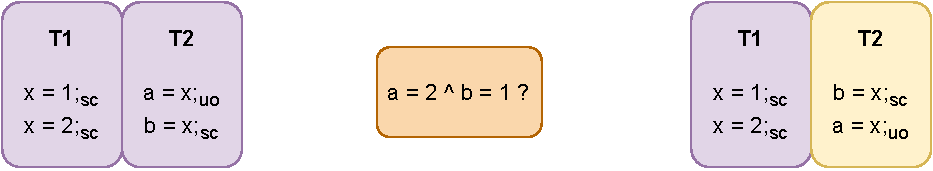
\includegraphics[scale=0.7]{5.InstructionReordering/0.Intro/ReorderingExample1(a).pdf}
            \caption{First example for reordering in candidates of the original program and its reordered counterpart.}
            \label{reord:example1(a)} 
        \end{figure}
        
        Figure~\ref{reord:example1(b)} has two sets of relations. 
        The first justifies the outcome for the reordered Candidate. 
        While the second justifies for the original Candidate. 
        Notice that in the first set of relations, we can infer that one may have a read memory ordered before a write that it reads from. 
        This is quite counter intuitive to understand at first. 
        But strictly from the semantics of the model, this justification to the observable behavior is completely valid\footnotemark. 
        \begin{figure}[H]
            \centering
            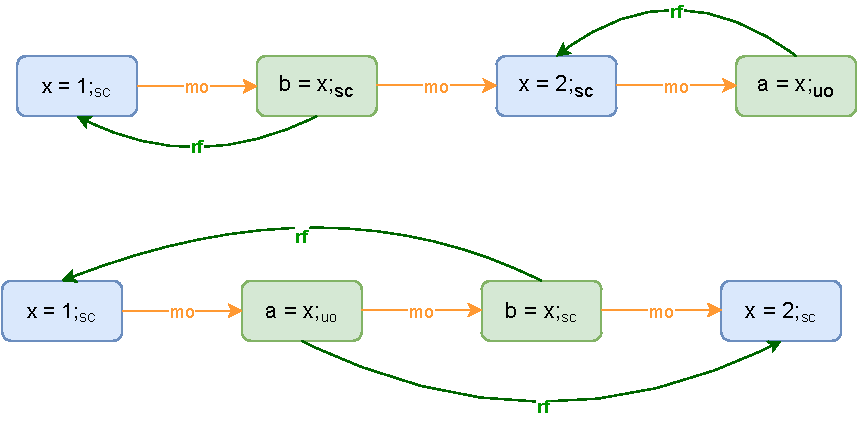
\includegraphics[scale=0.7]{5.InstructionReordering/0.Intro/ReorderingExample1(b).pdf}
            \caption{The set of partial order relations justifying the observable behavior in question for both the candidates in Figure~\ref{reord:example1(a)}.} 
            \label{reord:example1(b)}
        \end{figure}

        \footnotetext{In practice, this can be due to read speculation at the hardware level.}
        
        Consider another example in Figure~\ref{reord:example2(a)}.
        The figure on the left is the original candidate and that on the right is after reordering the two events of $T1$.
        The observable behavior in question is written in the middle(orange box). 
        \begin{figure}[H]
            \centering
            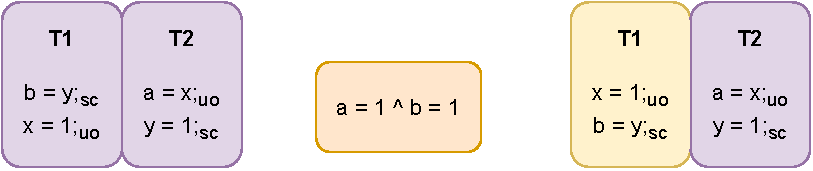
\includegraphics[scale=0.7]{5.InstructionReordering/0.Intro/ReorderingExample2(a).pdf}
            \caption{Second example for reordering with candidates of the original program and its reordered counterpart.} 
            \label{reord:example2(a)}
        \end{figure}
   
        Figure~\ref{reord:example2(b)} has two sets of relations. 
        The first justifies that such an outcome is not possible for the original program candidate due to Axiom \ref{CoRe}. 
        While the second justifies that this outcome is possible for the reordered program.
        Note that we cannot infer in the reordered candidate the set of relations for any candidate execution to have $\reln{a=x;_{uo}}{hb}{x=1;_{uo}}$. 
        \begin{figure}[H]
            \centering
            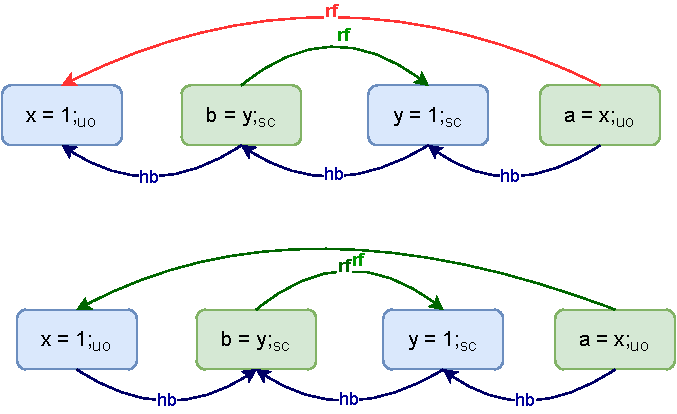
\includegraphics[scale=0.7]{5.InstructionReordering/0.Intro/ReorderingExample2(b).pdf}
            \caption{The set of partial order relations justifying the observable behavior in question for both the candidates in Figure~\ref{reord:example2(a)}.} 
            \label{reord:example2(b)}
        \end{figure}

        The above two examples show that we have to be careful while reordering two events in the same thread. 
        By example analysis, for each observable behavior, one must check all possible candidate executions and assert whether such an observable is possible or not. 
        This method of checking validity of reordering will scale exponentially as the program size increases. 
        It may also be the case that the compiler may not have information on which exact events would be executed in other threads to assert such reordering is valid. 

    
    
    
    
    

%Summary of Approach.
\section{Approach}

    We consider the same set of assumptions for reordering here. 
    Similar to reordering, our main objective is to ensure that the set of possible observable behaviors of a program, remain unchanged after elimination. 
    In the case of write elimination, the property we try to prove remains the same.
    In the case of read elimination though, we would want the observable behaviors excluding the specific read eliminated to be a subset.
    For both cases, if preserving all behaviors is not possible, then we would want the set of observable behaviors after elimination at the very least to be a subset.

    The main difference here is that elimination would remove certain happens-before relations, in contrast to having additional ones.
    From our point of view, we would want only the relations with the eliminated read/write to be removed after the transformation.
    The loss of these relations would certainly not have any new happens-before cycle introduced. 
    However, we still have to check whether the removed relations result in some new behavior. 
    We prove when it does not, by doing case-wise analysis on the type of relations eliminated.  

%Key definitions 
\section{Some Useful Definitions}
Before we go about proving when reordering is valid, we define certain helper definitions for it.

%Something we need to define for sake of proofs
\begin{definition}{Consecutive pair of events (\emph{cons})}
    \label{Cons}
    We define \emph{cons} as a function, which takes two events as input, and gives us a boolean indicating if they are consecutive pairs. Two events $e$ and $d$ are consecutive if they have a direct $\stck{_\textit{ao}}$ relation among them;  i.e those relations that are not derived through transitive property of $\stck{_\textit{hb}}$. 
    \begin{align*}
        (
        e \stck{_\textit{ao}} d  \ \wedge \ 
        \nexists k \ \textit{s.t.} \ 
        e \stck{_\textit{ao}} k  \ \wedge \
        k \stck{_\textit{ao}} d 
        )
        \ \vee \
        (
            d \stck{_\textit{ao}} e  \ \wedge \ 
            \nexists k \ \textit{s.t.} \ 
            d \stck{_\textit{ao}} k  \ \wedge \
            k \stck{_\textit{ao}} e  
        ).
    \end{align*}
\end{definition}

\begin{definition}{Direct happens-before relation (dir)}
    \label{Dir}
    We define \emph{dir} to take an ordered pair of events $(e,d)$ such that $\reln{e}{hb}{d}$ and gives a boolean value to indicate whether this relation is \textit{direct}, which can be formally stated as follows:
    \begin{align*}
        \nexists k \ \text{s.t.} \ \reln{e}{hb}{k} \wedge \reln{k}{hb}{d}.
    \end{align*}
    
    We can infer some useful things using \emph{dir} based on some information on events $e$ and $d$\footnotemark. 
    \begin{enumerate}
        \item If $\et{e}{uo}$, then $dir(e,d) \ \Rightarrow \ cons(e,d).$ 
        \item If $\et{d}{uo}$, then $dir(e,d) \ \Rightarrow \ cons(e,d).$
        \item If $\et{e}{sc}\ \wedge\ e\!\in\!R$, then $dir(e,d) \ \Rightarrow \ cons(e,d).$
        \item If $\et{e}{sc}\ \wedge\ e\!\in\!W$, then $dir(e,d) \ \Rightarrow \ cons(e,d)\ \vee\ \reln{e}{sw}{d}.$
        \item If $\et{d}{sc}\ \wedge\ d\!\in\!W$, then $dir(e,d) \ \Rightarrow \ cons(e,d).$
        \item If $\et{d}{sc}\ \wedge\ e\!\in\!R$, then $dir(e,d) \ \Rightarrow \ cons(e,d)\ \vee\ \reln{e}{sw}{d}.$
    \end{enumerate}

    \footnotetext{They can be proved trivially using definitions of $\stck{_{hb}}, \stck{_{sw}} \text{and} \stck{_{ao}}$}.
\end{definition}


\begin{definition}{Reorderable Pair (Reord)}
    \label{Reord}
    
    We define a boolean function \emph{Reord} that takes two ordered pair of events $(e,d)$ such that $\reln{e}{ao}{d}$ and gives a boolean value indicating if they are a reorderable pair\footnotemark.   
    \begin{align*}
        Reord(e,d) = \\
        (
        &((\et{e}{uo} \ \wedge \ \et{d}{uo}) \ \wedge \ 
                (   
                    (\event{e}{R} \ \wedge \ \event{d}{R}) \ \vee \ 
                    (\Re(e) \cap_\Re \Re(d) = \phi) 
                )
        ) \\ &\vee \\
        &((\et{e}{sc} \ \wedge \ \et{d}{uo}) \ \wedge \ 
                (
                    (\event{e}{W} \ \wedge \ (\Re(e) \cap_\Re \Re(d) = \phi)) 
                )
        ) \\ &\vee \\
        &((\et{e}{uo} \ \wedge \ \et{d}{sc}) \ \wedge \ 
                (
                    (\event{d}{R} \ \wedge \ (\Re(e) \cap_\Re \Re(d) = \phi)) 
                )
        )
        ).
    \end{align*}

    \footnotetext{We later prove that this exact definition defines when a pair of two consecutive events are reorderable.}
\end{definition}



%Key Lemmas 
This chapter addresses the validity of instruction reordering under the ECMAScript memory model.
We first start by showing some examples of Candidate Executions where reordering is not safe in the relaxed memory context.  
We give a brief summary of our approach towards a proof to identify when such a reordering is safe.
Next, we introduce a few more definitions for our purpose, followed by two lemmas that will be instrumental for proofs in this chapter and the next. 
We then formulate a theorem and a corresponding corollary that covers validity of reordering at a Candidate Execution level. 
Lastly, we address reordering at the program level involving conditional branching and loops.
We use counter examples to give a better intuitive understanding of the elements of the proof.
\ \newline
\ \newline  
\hrule 
\ \newline 
\ \newline 

\input{4.InstructionReordering/0.Intro/intro.tex}

%Summary of Approach.
\input{4.InstructionReordering/1.Approach.tex}

%Key definitions 
\input{4.InstructionReordering/2.Definitions.tex}

%Key Lemmas 
\input{4.InstructionReordering/3.Lemmas/main.tex}

%Valid reordering at the Candidate Execution level
\input{4.InstructionReordering/4.ValidReorderingCandidate/main.tex}

%From Candidates to Programs
\input{4.InstructionReordering/5.ValidReorderingProgram/main.tex}

%Conclusion (write here itself. No need for a new .tex file)
\ \newline
\ \newline  
\hrule 
\ \newline 
\ \newline 
To summarize, this chapter addressed the validity of instruction reordering under the ECMAScript Memory Model. 
We first built a conservative proof for reordering based on candidate executions.
We later extended it to programs abstracted to the set of shared memory events. 
We discussed throughout the limitation and advantages of our conservative approach. 
We also presented examples throughout this chapter to get a fair intuitive understanding of the ideas behind the proof and the role of the axiomatic model in it.
In the next chapter, we will address the validity of elimination under the ECMAScript Memory Model.

%Valid reordering at the Candidate Execution level
This chapter addresses the validity of instruction reordering under the ECMAScript memory model.
We first start by showing some examples of Candidate Executions where reordering is not safe in the relaxed memory context.  
We give a brief summary of our approach towards a proof to identify when such a reordering is safe.
Next, we introduce a few more definitions for our purpose, followed by two lemmas that will be instrumental for proofs in this chapter and the next. 
We then formulate a theorem and a corresponding corollary that covers validity of reordering at a Candidate Execution level. 
Lastly, we address reordering at the program level involving conditional branching and loops.
We use counter examples to give a better intuitive understanding of the elements of the proof.
\ \newline
\ \newline  
\hrule 
\ \newline 
\ \newline 

\input{4.InstructionReordering/0.Intro/intro.tex}

%Summary of Approach.
\input{4.InstructionReordering/1.Approach.tex}

%Key definitions 
\input{4.InstructionReordering/2.Definitions.tex}

%Key Lemmas 
\input{4.InstructionReordering/3.Lemmas/main.tex}

%Valid reordering at the Candidate Execution level
\input{4.InstructionReordering/4.ValidReorderingCandidate/main.tex}

%From Candidates to Programs
\input{4.InstructionReordering/5.ValidReorderingProgram/main.tex}

%Conclusion (write here itself. No need for a new .tex file)
\ \newline
\ \newline  
\hrule 
\ \newline 
\ \newline 
To summarize, this chapter addressed the validity of instruction reordering under the ECMAScript Memory Model. 
We first built a conservative proof for reordering based on candidate executions.
We later extended it to programs abstracted to the set of shared memory events. 
We discussed throughout the limitation and advantages of our conservative approach. 
We also presented examples throughout this chapter to get a fair intuitive understanding of the ideas behind the proof and the role of the axiomatic model in it.
In the next chapter, we will address the validity of elimination under the ECMAScript Memory Model.

%From Candidates to Programs
This chapter addresses the validity of instruction reordering under the ECMAScript memory model.
We first start by showing some examples of Candidate Executions where reordering is not safe in the relaxed memory context.  
We give a brief summary of our approach towards a proof to identify when such a reordering is safe.
Next, we introduce a few more definitions for our purpose, followed by two lemmas that will be instrumental for proofs in this chapter and the next. 
We then formulate a theorem and a corresponding corollary that covers validity of reordering at a Candidate Execution level. 
Lastly, we address reordering at the program level involving conditional branching and loops.
We use counter examples to give a better intuitive understanding of the elements of the proof.
\ \newline
\ \newline  
\hrule 
\ \newline 
\ \newline 

\input{4.InstructionReordering/0.Intro/intro.tex}

%Summary of Approach.
\input{4.InstructionReordering/1.Approach.tex}

%Key definitions 
\input{4.InstructionReordering/2.Definitions.tex}

%Key Lemmas 
\input{4.InstructionReordering/3.Lemmas/main.tex}

%Valid reordering at the Candidate Execution level
\input{4.InstructionReordering/4.ValidReorderingCandidate/main.tex}

%From Candidates to Programs
\input{4.InstructionReordering/5.ValidReorderingProgram/main.tex}

%Conclusion (write here itself. No need for a new .tex file)
\ \newline
\ \newline  
\hrule 
\ \newline 
\ \newline 
To summarize, this chapter addressed the validity of instruction reordering under the ECMAScript Memory Model. 
We first built a conservative proof for reordering based on candidate executions.
We later extended it to programs abstracted to the set of shared memory events. 
We discussed throughout the limitation and advantages of our conservative approach. 
We also presented examples throughout this chapter to get a fair intuitive understanding of the ideas behind the proof and the role of the axiomatic model in it.
In the next chapter, we will address the validity of elimination under the ECMAScript Memory Model.

%Conclusion (write here itself. No need for a new .tex file)
\ \newline
\ \newline  
\hrule 
\ \newline 
\ \newline 
To summarize, this chapter addressed the validity of instruction reordering under the ECMAScript Memory Model. 
We first built a conservative proof for reordering based on candidate executions.
We later extended it to programs abstracted to the set of shared memory events. 
We discussed throughout the limitation and advantages of our conservative approach. 
We also presented examples throughout this chapter to get a fair intuitive understanding of the ideas behind the proof and the role of the axiomatic model in it.
In the next chapter, we will address the validity of elimination under the ECMAScript Memory Model.

%From Candidates to Programs
This chapter addresses the validity of instruction reordering under the ECMAScript memory model.
We first start by showing some examples of Candidate Executions where reordering is not safe in the relaxed memory context.  
We give a brief summary of our approach towards a proof to identify when such a reordering is safe.
Next, we introduce a few more definitions for our purpose, followed by two lemmas that will be instrumental for proofs in this chapter and the next. 
We then formulate a theorem and a corresponding corollary that covers validity of reordering at a Candidate Execution level. 
Lastly, we address reordering at the program level involving conditional branching and loops.
We use counter examples to give a better intuitive understanding of the elements of the proof.
\ \newline
\ \newline  
\hrule 
\ \newline 
\ \newline 


\section{Introduction}
    Instruction reordering is a common transformation done by the compiler/hardware, which is essential to optimizations such as instruction scheduling, loop invariant removal, partial redundancy elimination, etc. 
    However, whether we can do such reordering freely given a concurrent program using relaxed memory accesses is a bit unclear. 
     
    \paragraph{Simple reordering is not straightforward under shared memory semantics}
    The main reason is that memory accesses here, do not just perform the desired operation (i.e Read / Write) but also imply certain visibility guarantees across all the other threads.  
    In our observation, we find that, the relaxed memory model of ECMAScript prescribe semantics for visibility using the $\stck{_{hb}}$ relations. 
    
    \paragraph{Some Examples}
        We show a couple of examples to showcase why reordering may not be that straightforward. 
        Consider the first example in Figure~\ref{reord:example1(a)} below of a Candidate before and after reordering two events.
        The original candidate is to the left and that on the right is after reordering the two reads of $T2$.
        The observable behavior in question is written in the middle(orange box). 
        \begin{figure}[H]
            \centering
            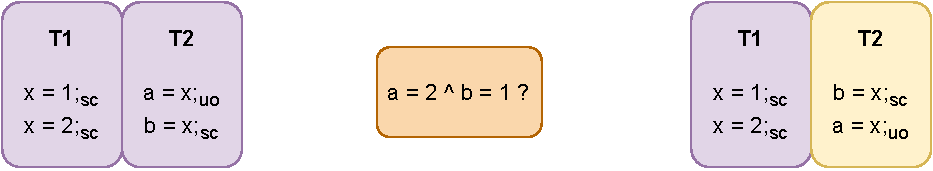
\includegraphics[scale=0.7]{5.InstructionReordering/0.Intro/ReorderingExample1(a).pdf}
            \caption{First example for reordering in candidates of the original program and its reordered counterpart.}
            \label{reord:example1(a)} 
        \end{figure}
        
        Figure~\ref{reord:example1(b)} has two sets of relations. 
        The first justifies the outcome for the reordered Candidate. 
        While the second justifies for the original Candidate. 
        Notice that in the first set of relations, we can infer that one may have a read memory ordered before a write that it reads from. 
        This is quite counter intuitive to understand at first. 
        But strictly from the semantics of the model, this justification to the observable behavior is completely valid\footnotemark. 
        \begin{figure}[H]
            \centering
            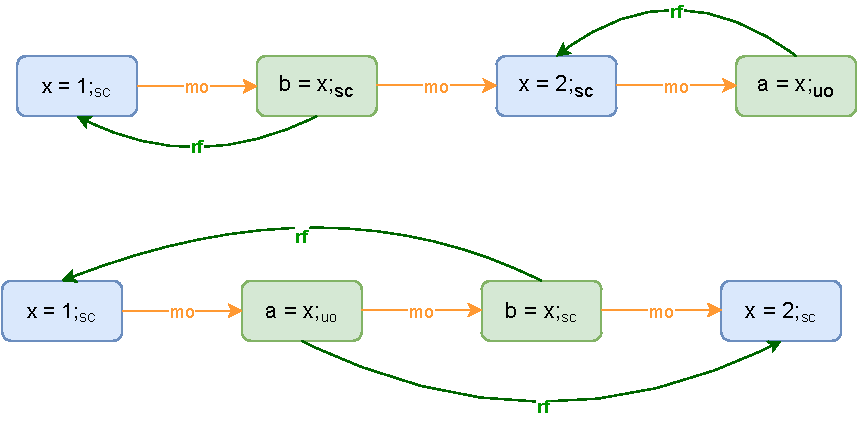
\includegraphics[scale=0.7]{5.InstructionReordering/0.Intro/ReorderingExample1(b).pdf}
            \caption{The set of partial order relations justifying the observable behavior in question for both the candidates in Figure~\ref{reord:example1(a)}.} 
            \label{reord:example1(b)}
        \end{figure}

        \footnotetext{In practice, this can be due to read speculation at the hardware level.}
        
        Consider another example in Figure~\ref{reord:example2(a)}.
        The figure on the left is the original candidate and that on the right is after reordering the two events of $T1$.
        The observable behavior in question is written in the middle(orange box). 
        \begin{figure}[H]
            \centering
            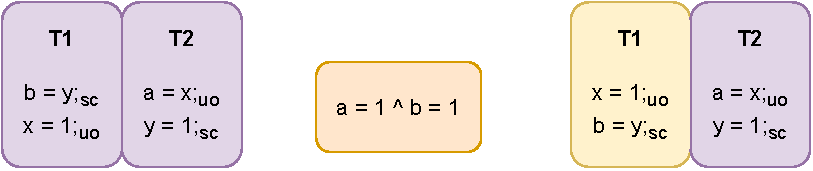
\includegraphics[scale=0.7]{5.InstructionReordering/0.Intro/ReorderingExample2(a).pdf}
            \caption{Second example for reordering with candidates of the original program and its reordered counterpart.} 
            \label{reord:example2(a)}
        \end{figure}
   
        Figure~\ref{reord:example2(b)} has two sets of relations. 
        The first justifies that such an outcome is not possible for the original program candidate due to Axiom \ref{CoRe}. 
        While the second justifies that this outcome is possible for the reordered program.
        Note that we cannot infer in the reordered candidate the set of relations for any candidate execution to have $\reln{a=x;_{uo}}{hb}{x=1;_{uo}}$. 
        \begin{figure}[H]
            \centering
            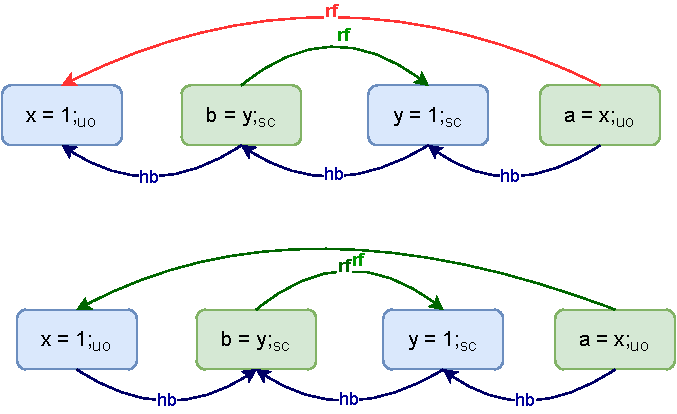
\includegraphics[scale=0.7]{5.InstructionReordering/0.Intro/ReorderingExample2(b).pdf}
            \caption{The set of partial order relations justifying the observable behavior in question for both the candidates in Figure~\ref{reord:example2(a)}.} 
            \label{reord:example2(b)}
        \end{figure}

        The above two examples show that we have to be careful while reordering two events in the same thread. 
        By example analysis, for each observable behavior, one must check all possible candidate executions and assert whether such an observable is possible or not. 
        This method of checking validity of reordering will scale exponentially as the program size increases. 
        It may also be the case that the compiler may not have information on which exact events would be executed in other threads to assert such reordering is valid. 

    
    
    
    
    

%Summary of Approach.
\section{Approach}

    We consider the same set of assumptions for reordering here. 
    Similar to reordering, our main objective is to ensure that the set of possible observable behaviors of a program, remain unchanged after elimination. 
    In the case of write elimination, the property we try to prove remains the same.
    In the case of read elimination though, we would want the observable behaviors excluding the specific read eliminated to be a subset.
    For both cases, if preserving all behaviors is not possible, then we would want the set of observable behaviors after elimination at the very least to be a subset.

    The main difference here is that elimination would remove certain happens-before relations, in contrast to having additional ones.
    From our point of view, we would want only the relations with the eliminated read/write to be removed after the transformation.
    The loss of these relations would certainly not have any new happens-before cycle introduced. 
    However, we still have to check whether the removed relations result in some new behavior. 
    We prove when it does not, by doing case-wise analysis on the type of relations eliminated.  

%Key definitions 
\section{Some Useful Definitions}
Before we go about proving when reordering is valid, we define certain helper definitions for it.

%Something we need to define for sake of proofs
\begin{definition}{Consecutive pair of events (\emph{cons})}
    \label{Cons}
    We define \emph{cons} as a function, which takes two events as input, and gives us a boolean indicating if they are consecutive pairs. Two events $e$ and $d$ are consecutive if they have a direct $\stck{_\textit{ao}}$ relation among them;  i.e those relations that are not derived through transitive property of $\stck{_\textit{hb}}$. 
    \begin{align*}
        (
        e \stck{_\textit{ao}} d  \ \wedge \ 
        \nexists k \ \textit{s.t.} \ 
        e \stck{_\textit{ao}} k  \ \wedge \
        k \stck{_\textit{ao}} d 
        )
        \ \vee \
        (
            d \stck{_\textit{ao}} e  \ \wedge \ 
            \nexists k \ \textit{s.t.} \ 
            d \stck{_\textit{ao}} k  \ \wedge \
            k \stck{_\textit{ao}} e  
        ).
    \end{align*}
\end{definition}

\begin{definition}{Direct happens-before relation (dir)}
    \label{Dir}
    We define \emph{dir} to take an ordered pair of events $(e,d)$ such that $\reln{e}{hb}{d}$ and gives a boolean value to indicate whether this relation is \textit{direct}, which can be formally stated as follows:
    \begin{align*}
        \nexists k \ \text{s.t.} \ \reln{e}{hb}{k} \wedge \reln{k}{hb}{d}.
    \end{align*}
    
    We can infer some useful things using \emph{dir} based on some information on events $e$ and $d$\footnotemark. 
    \begin{enumerate}
        \item If $\et{e}{uo}$, then $dir(e,d) \ \Rightarrow \ cons(e,d).$ 
        \item If $\et{d}{uo}$, then $dir(e,d) \ \Rightarrow \ cons(e,d).$
        \item If $\et{e}{sc}\ \wedge\ e\!\in\!R$, then $dir(e,d) \ \Rightarrow \ cons(e,d).$
        \item If $\et{e}{sc}\ \wedge\ e\!\in\!W$, then $dir(e,d) \ \Rightarrow \ cons(e,d)\ \vee\ \reln{e}{sw}{d}.$
        \item If $\et{d}{sc}\ \wedge\ d\!\in\!W$, then $dir(e,d) \ \Rightarrow \ cons(e,d).$
        \item If $\et{d}{sc}\ \wedge\ e\!\in\!R$, then $dir(e,d) \ \Rightarrow \ cons(e,d)\ \vee\ \reln{e}{sw}{d}.$
    \end{enumerate}

    \footnotetext{They can be proved trivially using definitions of $\stck{_{hb}}, \stck{_{sw}} \text{and} \stck{_{ao}}$}.
\end{definition}


\begin{definition}{Reorderable Pair (Reord)}
    \label{Reord}
    
    We define a boolean function \emph{Reord} that takes two ordered pair of events $(e,d)$ such that $\reln{e}{ao}{d}$ and gives a boolean value indicating if they are a reorderable pair\footnotemark.   
    \begin{align*}
        Reord(e,d) = \\
        (
        &((\et{e}{uo} \ \wedge \ \et{d}{uo}) \ \wedge \ 
                (   
                    (\event{e}{R} \ \wedge \ \event{d}{R}) \ \vee \ 
                    (\Re(e) \cap_\Re \Re(d) = \phi) 
                )
        ) \\ &\vee \\
        &((\et{e}{sc} \ \wedge \ \et{d}{uo}) \ \wedge \ 
                (
                    (\event{e}{W} \ \wedge \ (\Re(e) \cap_\Re \Re(d) = \phi)) 
                )
        ) \\ &\vee \\
        &((\et{e}{uo} \ \wedge \ \et{d}{sc}) \ \wedge \ 
                (
                    (\event{d}{R} \ \wedge \ (\Re(e) \cap_\Re \Re(d) = \phi)) 
                )
        )
        ).
    \end{align*}

    \footnotetext{We later prove that this exact definition defines when a pair of two consecutive events are reorderable.}
\end{definition}



%Key Lemmas 
This chapter addresses the validity of instruction reordering under the ECMAScript memory model.
We first start by showing some examples of Candidate Executions where reordering is not safe in the relaxed memory context.  
We give a brief summary of our approach towards a proof to identify when such a reordering is safe.
Next, we introduce a few more definitions for our purpose, followed by two lemmas that will be instrumental for proofs in this chapter and the next. 
We then formulate a theorem and a corresponding corollary that covers validity of reordering at a Candidate Execution level. 
Lastly, we address reordering at the program level involving conditional branching and loops.
We use counter examples to give a better intuitive understanding of the elements of the proof.
\ \newline
\ \newline  
\hrule 
\ \newline 
\ \newline 

\input{4.InstructionReordering/0.Intro/intro.tex}

%Summary of Approach.
\input{4.InstructionReordering/1.Approach.tex}

%Key definitions 
\input{4.InstructionReordering/2.Definitions.tex}

%Key Lemmas 
\input{4.InstructionReordering/3.Lemmas/main.tex}

%Valid reordering at the Candidate Execution level
\input{4.InstructionReordering/4.ValidReorderingCandidate/main.tex}

%From Candidates to Programs
\input{4.InstructionReordering/5.ValidReorderingProgram/main.tex}

%Conclusion (write here itself. No need for a new .tex file)
\ \newline
\ \newline  
\hrule 
\ \newline 
\ \newline 
To summarize, this chapter addressed the validity of instruction reordering under the ECMAScript Memory Model. 
We first built a conservative proof for reordering based on candidate executions.
We later extended it to programs abstracted to the set of shared memory events. 
We discussed throughout the limitation and advantages of our conservative approach. 
We also presented examples throughout this chapter to get a fair intuitive understanding of the ideas behind the proof and the role of the axiomatic model in it.
In the next chapter, we will address the validity of elimination under the ECMAScript Memory Model.

%Valid reordering at the Candidate Execution level
This chapter addresses the validity of instruction reordering under the ECMAScript memory model.
We first start by showing some examples of Candidate Executions where reordering is not safe in the relaxed memory context.  
We give a brief summary of our approach towards a proof to identify when such a reordering is safe.
Next, we introduce a few more definitions for our purpose, followed by two lemmas that will be instrumental for proofs in this chapter and the next. 
We then formulate a theorem and a corresponding corollary that covers validity of reordering at a Candidate Execution level. 
Lastly, we address reordering at the program level involving conditional branching and loops.
We use counter examples to give a better intuitive understanding of the elements of the proof.
\ \newline
\ \newline  
\hrule 
\ \newline 
\ \newline 

\input{4.InstructionReordering/0.Intro/intro.tex}

%Summary of Approach.
\input{4.InstructionReordering/1.Approach.tex}

%Key definitions 
\input{4.InstructionReordering/2.Definitions.tex}

%Key Lemmas 
\input{4.InstructionReordering/3.Lemmas/main.tex}

%Valid reordering at the Candidate Execution level
\input{4.InstructionReordering/4.ValidReorderingCandidate/main.tex}

%From Candidates to Programs
\input{4.InstructionReordering/5.ValidReorderingProgram/main.tex}

%Conclusion (write here itself. No need for a new .tex file)
\ \newline
\ \newline  
\hrule 
\ \newline 
\ \newline 
To summarize, this chapter addressed the validity of instruction reordering under the ECMAScript Memory Model. 
We first built a conservative proof for reordering based on candidate executions.
We later extended it to programs abstracted to the set of shared memory events. 
We discussed throughout the limitation and advantages of our conservative approach. 
We also presented examples throughout this chapter to get a fair intuitive understanding of the ideas behind the proof and the role of the axiomatic model in it.
In the next chapter, we will address the validity of elimination under the ECMAScript Memory Model.

%From Candidates to Programs
This chapter addresses the validity of instruction reordering under the ECMAScript memory model.
We first start by showing some examples of Candidate Executions where reordering is not safe in the relaxed memory context.  
We give a brief summary of our approach towards a proof to identify when such a reordering is safe.
Next, we introduce a few more definitions for our purpose, followed by two lemmas that will be instrumental for proofs in this chapter and the next. 
We then formulate a theorem and a corresponding corollary that covers validity of reordering at a Candidate Execution level. 
Lastly, we address reordering at the program level involving conditional branching and loops.
We use counter examples to give a better intuitive understanding of the elements of the proof.
\ \newline
\ \newline  
\hrule 
\ \newline 
\ \newline 

\input{4.InstructionReordering/0.Intro/intro.tex}

%Summary of Approach.
\input{4.InstructionReordering/1.Approach.tex}

%Key definitions 
\input{4.InstructionReordering/2.Definitions.tex}

%Key Lemmas 
\input{4.InstructionReordering/3.Lemmas/main.tex}

%Valid reordering at the Candidate Execution level
\input{4.InstructionReordering/4.ValidReorderingCandidate/main.tex}

%From Candidates to Programs
\input{4.InstructionReordering/5.ValidReorderingProgram/main.tex}

%Conclusion (write here itself. No need for a new .tex file)
\ \newline
\ \newline  
\hrule 
\ \newline 
\ \newline 
To summarize, this chapter addressed the validity of instruction reordering under the ECMAScript Memory Model. 
We first built a conservative proof for reordering based on candidate executions.
We later extended it to programs abstracted to the set of shared memory events. 
We discussed throughout the limitation and advantages of our conservative approach. 
We also presented examples throughout this chapter to get a fair intuitive understanding of the ideas behind the proof and the role of the axiomatic model in it.
In the next chapter, we will address the validity of elimination under the ECMAScript Memory Model.

%Conclusion (write here itself. No need for a new .tex file)
\ \newline
\ \newline  
\hrule 
\ \newline 
\ \newline 
To summarize, this chapter addressed the validity of instruction reordering under the ECMAScript Memory Model. 
We first built a conservative proof for reordering based on candidate executions.
We later extended it to programs abstracted to the set of shared memory events. 
We discussed throughout the limitation and advantages of our conservative approach. 
We also presented examples throughout this chapter to get a fair intuitive understanding of the ideas behind the proof and the role of the axiomatic model in it.
In the next chapter, we will address the validity of elimination under the ECMAScript Memory Model.

%Conclusion (write here itself. No need for a new .tex file)
\ \newline
\ \newline  
\hrule 
\ \newline 
\ \newline 
To summarize, this chapter addressed the validity of instruction reordering under the ECMAScript Memory Model. 
We first built a conservative proof for reordering based on candidate executions.
We later extended it to programs abstracted to the set of shared memory events. 
We discussed throughout the limitation and advantages of our conservative approach. 
We also presented examples throughout this chapter to get a fair intuitive understanding of the ideas behind the proof and the role of the axiomatic model in it.
In the next chapter, we will address the validity of elimination under the ECMAScript Memory Model.

%From Candidates to Programs
This chapter addresses the validity of instruction reordering under the ECMAScript memory model.
We first start by showing some examples of Candidate Executions where reordering is not safe in the relaxed memory context.  
We give a brief summary of our approach towards a proof to identify when such a reordering is safe.
Next, we introduce a few more definitions for our purpose, followed by two lemmas that will be instrumental for proofs in this chapter and the next. 
We then formulate a theorem and a corresponding corollary that covers validity of reordering at a Candidate Execution level. 
Lastly, we address reordering at the program level involving conditional branching and loops.
We use counter examples to give a better intuitive understanding of the elements of the proof.
\ \newline
\ \newline  
\hrule 
\ \newline 
\ \newline 


\section{Introduction}
    Instruction reordering is a common transformation done by the compiler/hardware, which is essential to optimizations such as instruction scheduling, loop invariant removal, partial redundancy elimination, etc. 
    However, whether we can do such reordering freely given a concurrent program using relaxed memory accesses is a bit unclear. 
     
    \paragraph{Simple reordering is not straightforward under shared memory semantics}
    The main reason is that memory accesses here, do not just perform the desired operation (i.e Read / Write) but also imply certain visibility guarantees across all the other threads.  
    In our observation, we find that, the relaxed memory model of ECMAScript prescribe semantics for visibility using the $\stck{_{hb}}$ relations. 
    
    \paragraph{Some Examples}
        We show a couple of examples to showcase why reordering may not be that straightforward. 
        Consider the first example in Figure~\ref{reord:example1(a)} below of a Candidate before and after reordering two events.
        The original candidate is to the left and that on the right is after reordering the two reads of $T2$.
        The observable behavior in question is written in the middle(orange box). 
        \begin{figure}[H]
            \centering
            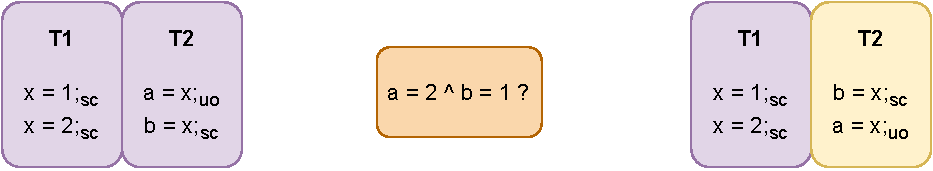
\includegraphics[scale=0.7]{5.InstructionReordering/0.Intro/ReorderingExample1(a).pdf}
            \caption{First example for reordering in candidates of the original program and its reordered counterpart.}
            \label{reord:example1(a)} 
        \end{figure}
        
        Figure~\ref{reord:example1(b)} has two sets of relations. 
        The first justifies the outcome for the reordered Candidate. 
        While the second justifies for the original Candidate. 
        Notice that in the first set of relations, we can infer that one may have a read memory ordered before a write that it reads from. 
        This is quite counter intuitive to understand at first. 
        But strictly from the semantics of the model, this justification to the observable behavior is completely valid\footnotemark. 
        \begin{figure}[H]
            \centering
            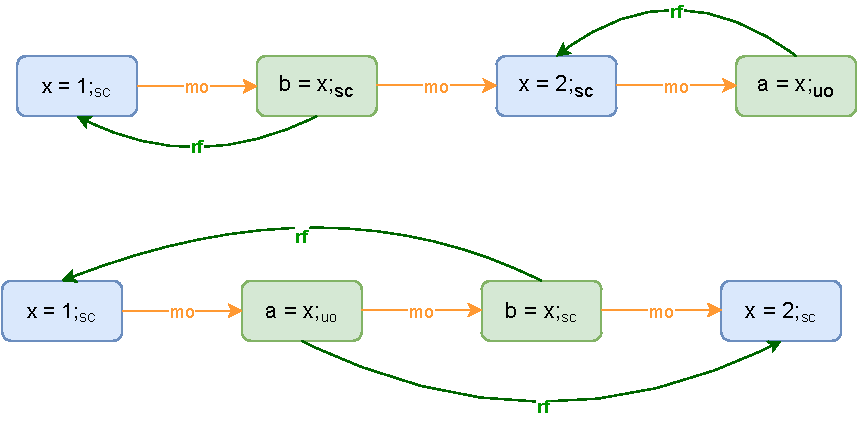
\includegraphics[scale=0.7]{5.InstructionReordering/0.Intro/ReorderingExample1(b).pdf}
            \caption{The set of partial order relations justifying the observable behavior in question for both the candidates in Figure~\ref{reord:example1(a)}.} 
            \label{reord:example1(b)}
        \end{figure}

        \footnotetext{In practice, this can be due to read speculation at the hardware level.}
        
        Consider another example in Figure~\ref{reord:example2(a)}.
        The figure on the left is the original candidate and that on the right is after reordering the two events of $T1$.
        The observable behavior in question is written in the middle(orange box). 
        \begin{figure}[H]
            \centering
            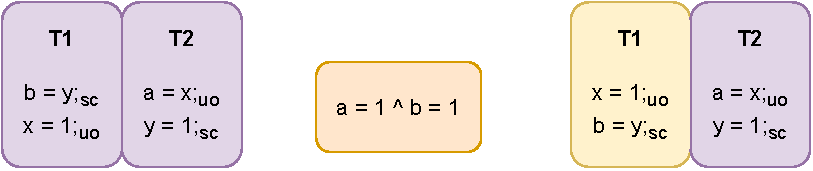
\includegraphics[scale=0.7]{5.InstructionReordering/0.Intro/ReorderingExample2(a).pdf}
            \caption{Second example for reordering with candidates of the original program and its reordered counterpart.} 
            \label{reord:example2(a)}
        \end{figure}
   
        Figure~\ref{reord:example2(b)} has two sets of relations. 
        The first justifies that such an outcome is not possible for the original program candidate due to Axiom \ref{CoRe}. 
        While the second justifies that this outcome is possible for the reordered program.
        Note that we cannot infer in the reordered candidate the set of relations for any candidate execution to have $\reln{a=x;_{uo}}{hb}{x=1;_{uo}}$. 
        \begin{figure}[H]
            \centering
            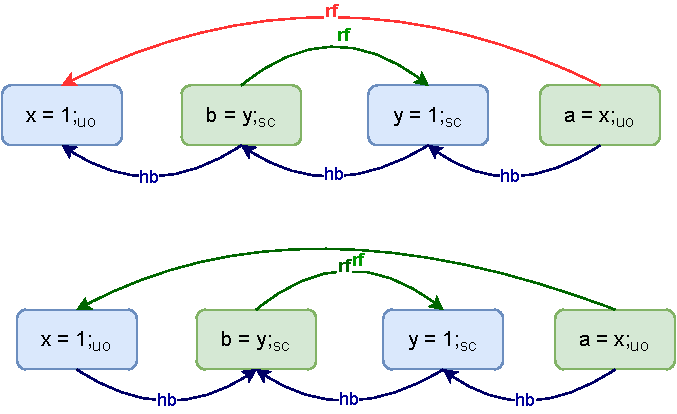
\includegraphics[scale=0.7]{5.InstructionReordering/0.Intro/ReorderingExample2(b).pdf}
            \caption{The set of partial order relations justifying the observable behavior in question for both the candidates in Figure~\ref{reord:example2(a)}.} 
            \label{reord:example2(b)}
        \end{figure}

        The above two examples show that we have to be careful while reordering two events in the same thread. 
        By example analysis, for each observable behavior, one must check all possible candidate executions and assert whether such an observable is possible or not. 
        This method of checking validity of reordering will scale exponentially as the program size increases. 
        It may also be the case that the compiler may not have information on which exact events would be executed in other threads to assert such reordering is valid. 

    
    
    
    
    

%Summary of Approach.
\section{Approach}

    We consider the same set of assumptions for reordering here. 
    Similar to reordering, our main objective is to ensure that the set of possible observable behaviors of a program, remain unchanged after elimination. 
    In the case of write elimination, the property we try to prove remains the same.
    In the case of read elimination though, we would want the observable behaviors excluding the specific read eliminated to be a subset.
    For both cases, if preserving all behaviors is not possible, then we would want the set of observable behaviors after elimination at the very least to be a subset.

    The main difference here is that elimination would remove certain happens-before relations, in contrast to having additional ones.
    From our point of view, we would want only the relations with the eliminated read/write to be removed after the transformation.
    The loss of these relations would certainly not have any new happens-before cycle introduced. 
    However, we still have to check whether the removed relations result in some new behavior. 
    We prove when it does not, by doing case-wise analysis on the type of relations eliminated.  

%Key definitions 
\section{Some Useful Definitions}
Before we go about proving when reordering is valid, we define certain helper definitions for it.

%Something we need to define for sake of proofs
\begin{definition}{Consecutive pair of events (\emph{cons})}
    \label{Cons}
    We define \emph{cons} as a function, which takes two events as input, and gives us a boolean indicating if they are consecutive pairs. Two events $e$ and $d$ are consecutive if they have a direct $\stck{_\textit{ao}}$ relation among them;  i.e those relations that are not derived through transitive property of $\stck{_\textit{hb}}$. 
    \begin{align*}
        (
        e \stck{_\textit{ao}} d  \ \wedge \ 
        \nexists k \ \textit{s.t.} \ 
        e \stck{_\textit{ao}} k  \ \wedge \
        k \stck{_\textit{ao}} d 
        )
        \ \vee \
        (
            d \stck{_\textit{ao}} e  \ \wedge \ 
            \nexists k \ \textit{s.t.} \ 
            d \stck{_\textit{ao}} k  \ \wedge \
            k \stck{_\textit{ao}} e  
        ).
    \end{align*}
\end{definition}

\begin{definition}{Direct happens-before relation (dir)}
    \label{Dir}
    We define \emph{dir} to take an ordered pair of events $(e,d)$ such that $\reln{e}{hb}{d}$ and gives a boolean value to indicate whether this relation is \textit{direct}, which can be formally stated as follows:
    \begin{align*}
        \nexists k \ \text{s.t.} \ \reln{e}{hb}{k} \wedge \reln{k}{hb}{d}.
    \end{align*}
    
    We can infer some useful things using \emph{dir} based on some information on events $e$ and $d$\footnotemark. 
    \begin{enumerate}
        \item If $\et{e}{uo}$, then $dir(e,d) \ \Rightarrow \ cons(e,d).$ 
        \item If $\et{d}{uo}$, then $dir(e,d) \ \Rightarrow \ cons(e,d).$
        \item If $\et{e}{sc}\ \wedge\ e\!\in\!R$, then $dir(e,d) \ \Rightarrow \ cons(e,d).$
        \item If $\et{e}{sc}\ \wedge\ e\!\in\!W$, then $dir(e,d) \ \Rightarrow \ cons(e,d)\ \vee\ \reln{e}{sw}{d}.$
        \item If $\et{d}{sc}\ \wedge\ d\!\in\!W$, then $dir(e,d) \ \Rightarrow \ cons(e,d).$
        \item If $\et{d}{sc}\ \wedge\ e\!\in\!R$, then $dir(e,d) \ \Rightarrow \ cons(e,d)\ \vee\ \reln{e}{sw}{d}.$
    \end{enumerate}

    \footnotetext{They can be proved trivially using definitions of $\stck{_{hb}}, \stck{_{sw}} \text{and} \stck{_{ao}}$}.
\end{definition}


\begin{definition}{Reorderable Pair (Reord)}
    \label{Reord}
    
    We define a boolean function \emph{Reord} that takes two ordered pair of events $(e,d)$ such that $\reln{e}{ao}{d}$ and gives a boolean value indicating if they are a reorderable pair\footnotemark.   
    \begin{align*}
        Reord(e,d) = \\
        (
        &((\et{e}{uo} \ \wedge \ \et{d}{uo}) \ \wedge \ 
                (   
                    (\event{e}{R} \ \wedge \ \event{d}{R}) \ \vee \ 
                    (\Re(e) \cap_\Re \Re(d) = \phi) 
                )
        ) \\ &\vee \\
        &((\et{e}{sc} \ \wedge \ \et{d}{uo}) \ \wedge \ 
                (
                    (\event{e}{W} \ \wedge \ (\Re(e) \cap_\Re \Re(d) = \phi)) 
                )
        ) \\ &\vee \\
        &((\et{e}{uo} \ \wedge \ \et{d}{sc}) \ \wedge \ 
                (
                    (\event{d}{R} \ \wedge \ (\Re(e) \cap_\Re \Re(d) = \phi)) 
                )
        )
        ).
    \end{align*}

    \footnotetext{We later prove that this exact definition defines when a pair of two consecutive events are reorderable.}
\end{definition}



%Key Lemmas 
This chapter addresses the validity of instruction reordering under the ECMAScript memory model.
We first start by showing some examples of Candidate Executions where reordering is not safe in the relaxed memory context.  
We give a brief summary of our approach towards a proof to identify when such a reordering is safe.
Next, we introduce a few more definitions for our purpose, followed by two lemmas that will be instrumental for proofs in this chapter and the next. 
We then formulate a theorem and a corresponding corollary that covers validity of reordering at a Candidate Execution level. 
Lastly, we address reordering at the program level involving conditional branching and loops.
We use counter examples to give a better intuitive understanding of the elements of the proof.
\ \newline
\ \newline  
\hrule 
\ \newline 
\ \newline 


\section{Introduction}
    Instruction reordering is a common transformation done by the compiler/hardware, which is essential to optimizations such as instruction scheduling, loop invariant removal, partial redundancy elimination, etc. 
    However, whether we can do such reordering freely given a concurrent program using relaxed memory accesses is a bit unclear. 
     
    \paragraph{Simple reordering is not straightforward under shared memory semantics}
    The main reason is that memory accesses here, do not just perform the desired operation (i.e Read / Write) but also imply certain visibility guarantees across all the other threads.  
    In our observation, we find that, the relaxed memory model of ECMAScript prescribe semantics for visibility using the $\stck{_{hb}}$ relations. 
    
    \paragraph{Some Examples}
        We show a couple of examples to showcase why reordering may not be that straightforward. 
        Consider the first example in Figure~\ref{reord:example1(a)} below of a Candidate before and after reordering two events.
        The original candidate is to the left and that on the right is after reordering the two reads of $T2$.
        The observable behavior in question is written in the middle(orange box). 
        \begin{figure}[H]
            \centering
            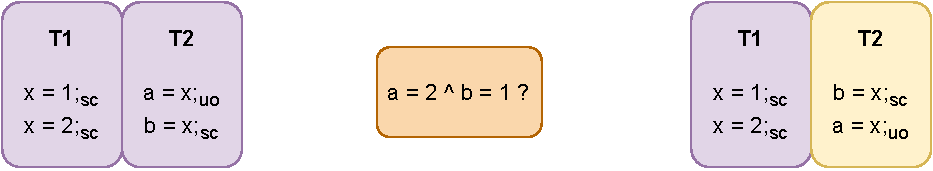
\includegraphics[scale=0.7]{5.InstructionReordering/0.Intro/ReorderingExample1(a).pdf}
            \caption{First example for reordering in candidates of the original program and its reordered counterpart.}
            \label{reord:example1(a)} 
        \end{figure}
        
        Figure~\ref{reord:example1(b)} has two sets of relations. 
        The first justifies the outcome for the reordered Candidate. 
        While the second justifies for the original Candidate. 
        Notice that in the first set of relations, we can infer that one may have a read memory ordered before a write that it reads from. 
        This is quite counter intuitive to understand at first. 
        But strictly from the semantics of the model, this justification to the observable behavior is completely valid\footnotemark. 
        \begin{figure}[H]
            \centering
            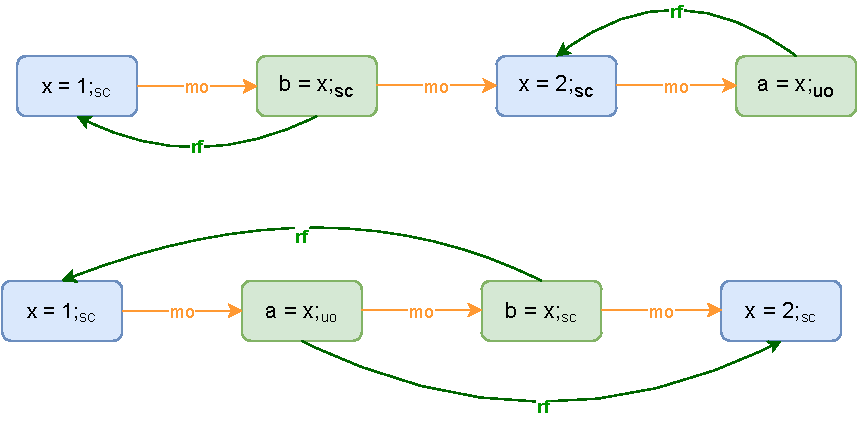
\includegraphics[scale=0.7]{5.InstructionReordering/0.Intro/ReorderingExample1(b).pdf}
            \caption{The set of partial order relations justifying the observable behavior in question for both the candidates in Figure~\ref{reord:example1(a)}.} 
            \label{reord:example1(b)}
        \end{figure}

        \footnotetext{In practice, this can be due to read speculation at the hardware level.}
        
        Consider another example in Figure~\ref{reord:example2(a)}.
        The figure on the left is the original candidate and that on the right is after reordering the two events of $T1$.
        The observable behavior in question is written in the middle(orange box). 
        \begin{figure}[H]
            \centering
            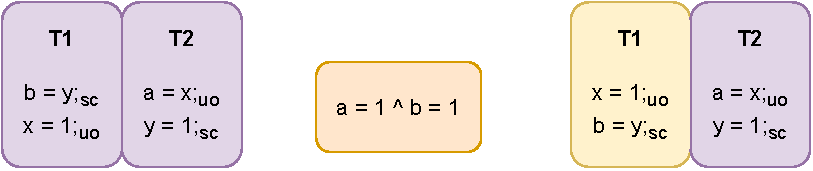
\includegraphics[scale=0.7]{5.InstructionReordering/0.Intro/ReorderingExample2(a).pdf}
            \caption{Second example for reordering with candidates of the original program and its reordered counterpart.} 
            \label{reord:example2(a)}
        \end{figure}
   
        Figure~\ref{reord:example2(b)} has two sets of relations. 
        The first justifies that such an outcome is not possible for the original program candidate due to Axiom \ref{CoRe}. 
        While the second justifies that this outcome is possible for the reordered program.
        Note that we cannot infer in the reordered candidate the set of relations for any candidate execution to have $\reln{a=x;_{uo}}{hb}{x=1;_{uo}}$. 
        \begin{figure}[H]
            \centering
            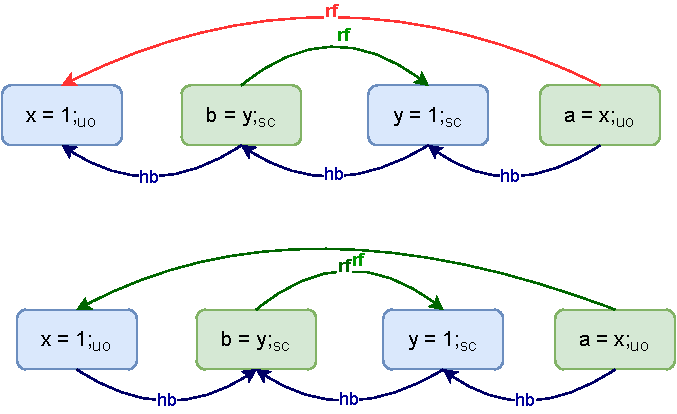
\includegraphics[scale=0.7]{5.InstructionReordering/0.Intro/ReorderingExample2(b).pdf}
            \caption{The set of partial order relations justifying the observable behavior in question for both the candidates in Figure~\ref{reord:example2(a)}.} 
            \label{reord:example2(b)}
        \end{figure}

        The above two examples show that we have to be careful while reordering two events in the same thread. 
        By example analysis, for each observable behavior, one must check all possible candidate executions and assert whether such an observable is possible or not. 
        This method of checking validity of reordering will scale exponentially as the program size increases. 
        It may also be the case that the compiler may not have information on which exact events would be executed in other threads to assert such reordering is valid. 

    
    
    
    
    

%Summary of Approach.
\section{Approach}

    We consider the same set of assumptions for reordering here. 
    Similar to reordering, our main objective is to ensure that the set of possible observable behaviors of a program, remain unchanged after elimination. 
    In the case of write elimination, the property we try to prove remains the same.
    In the case of read elimination though, we would want the observable behaviors excluding the specific read eliminated to be a subset.
    For both cases, if preserving all behaviors is not possible, then we would want the set of observable behaviors after elimination at the very least to be a subset.

    The main difference here is that elimination would remove certain happens-before relations, in contrast to having additional ones.
    From our point of view, we would want only the relations with the eliminated read/write to be removed after the transformation.
    The loss of these relations would certainly not have any new happens-before cycle introduced. 
    However, we still have to check whether the removed relations result in some new behavior. 
    We prove when it does not, by doing case-wise analysis on the type of relations eliminated.  

%Key definitions 
\section{Some Useful Definitions}
Before we go about proving when reordering is valid, we define certain helper definitions for it.

%Something we need to define for sake of proofs
\begin{definition}{Consecutive pair of events (\emph{cons})}
    \label{Cons}
    We define \emph{cons} as a function, which takes two events as input, and gives us a boolean indicating if they are consecutive pairs. Two events $e$ and $d$ are consecutive if they have a direct $\stck{_\textit{ao}}$ relation among them;  i.e those relations that are not derived through transitive property of $\stck{_\textit{hb}}$. 
    \begin{align*}
        (
        e \stck{_\textit{ao}} d  \ \wedge \ 
        \nexists k \ \textit{s.t.} \ 
        e \stck{_\textit{ao}} k  \ \wedge \
        k \stck{_\textit{ao}} d 
        )
        \ \vee \
        (
            d \stck{_\textit{ao}} e  \ \wedge \ 
            \nexists k \ \textit{s.t.} \ 
            d \stck{_\textit{ao}} k  \ \wedge \
            k \stck{_\textit{ao}} e  
        ).
    \end{align*}
\end{definition}

\begin{definition}{Direct happens-before relation (dir)}
    \label{Dir}
    We define \emph{dir} to take an ordered pair of events $(e,d)$ such that $\reln{e}{hb}{d}$ and gives a boolean value to indicate whether this relation is \textit{direct}, which can be formally stated as follows:
    \begin{align*}
        \nexists k \ \text{s.t.} \ \reln{e}{hb}{k} \wedge \reln{k}{hb}{d}.
    \end{align*}
    
    We can infer some useful things using \emph{dir} based on some information on events $e$ and $d$\footnotemark. 
    \begin{enumerate}
        \item If $\et{e}{uo}$, then $dir(e,d) \ \Rightarrow \ cons(e,d).$ 
        \item If $\et{d}{uo}$, then $dir(e,d) \ \Rightarrow \ cons(e,d).$
        \item If $\et{e}{sc}\ \wedge\ e\!\in\!R$, then $dir(e,d) \ \Rightarrow \ cons(e,d).$
        \item If $\et{e}{sc}\ \wedge\ e\!\in\!W$, then $dir(e,d) \ \Rightarrow \ cons(e,d)\ \vee\ \reln{e}{sw}{d}.$
        \item If $\et{d}{sc}\ \wedge\ d\!\in\!W$, then $dir(e,d) \ \Rightarrow \ cons(e,d).$
        \item If $\et{d}{sc}\ \wedge\ e\!\in\!R$, then $dir(e,d) \ \Rightarrow \ cons(e,d)\ \vee\ \reln{e}{sw}{d}.$
    \end{enumerate}

    \footnotetext{They can be proved trivially using definitions of $\stck{_{hb}}, \stck{_{sw}} \text{and} \stck{_{ao}}$}.
\end{definition}


\begin{definition}{Reorderable Pair (Reord)}
    \label{Reord}
    
    We define a boolean function \emph{Reord} that takes two ordered pair of events $(e,d)$ such that $\reln{e}{ao}{d}$ and gives a boolean value indicating if they are a reorderable pair\footnotemark.   
    \begin{align*}
        Reord(e,d) = \\
        (
        &((\et{e}{uo} \ \wedge \ \et{d}{uo}) \ \wedge \ 
                (   
                    (\event{e}{R} \ \wedge \ \event{d}{R}) \ \vee \ 
                    (\Re(e) \cap_\Re \Re(d) = \phi) 
                )
        ) \\ &\vee \\
        &((\et{e}{sc} \ \wedge \ \et{d}{uo}) \ \wedge \ 
                (
                    (\event{e}{W} \ \wedge \ (\Re(e) \cap_\Re \Re(d) = \phi)) 
                )
        ) \\ &\vee \\
        &((\et{e}{uo} \ \wedge \ \et{d}{sc}) \ \wedge \ 
                (
                    (\event{d}{R} \ \wedge \ (\Re(e) \cap_\Re \Re(d) = \phi)) 
                )
        )
        ).
    \end{align*}

    \footnotetext{We later prove that this exact definition defines when a pair of two consecutive events are reorderable.}
\end{definition}



%Key Lemmas 
This chapter addresses the validity of instruction reordering under the ECMAScript memory model.
We first start by showing some examples of Candidate Executions where reordering is not safe in the relaxed memory context.  
We give a brief summary of our approach towards a proof to identify when such a reordering is safe.
Next, we introduce a few more definitions for our purpose, followed by two lemmas that will be instrumental for proofs in this chapter and the next. 
We then formulate a theorem and a corresponding corollary that covers validity of reordering at a Candidate Execution level. 
Lastly, we address reordering at the program level involving conditional branching and loops.
We use counter examples to give a better intuitive understanding of the elements of the proof.
\ \newline
\ \newline  
\hrule 
\ \newline 
\ \newline 

\input{4.InstructionReordering/0.Intro/intro.tex}

%Summary of Approach.
\input{4.InstructionReordering/1.Approach.tex}

%Key definitions 
\input{4.InstructionReordering/2.Definitions.tex}

%Key Lemmas 
\input{4.InstructionReordering/3.Lemmas/main.tex}

%Valid reordering at the Candidate Execution level
\input{4.InstructionReordering/4.ValidReorderingCandidate/main.tex}

%From Candidates to Programs
\input{4.InstructionReordering/5.ValidReorderingProgram/main.tex}

%Conclusion (write here itself. No need for a new .tex file)
\ \newline
\ \newline  
\hrule 
\ \newline 
\ \newline 
To summarize, this chapter addressed the validity of instruction reordering under the ECMAScript Memory Model. 
We first built a conservative proof for reordering based on candidate executions.
We later extended it to programs abstracted to the set of shared memory events. 
We discussed throughout the limitation and advantages of our conservative approach. 
We also presented examples throughout this chapter to get a fair intuitive understanding of the ideas behind the proof and the role of the axiomatic model in it.
In the next chapter, we will address the validity of elimination under the ECMAScript Memory Model.

%Valid reordering at the Candidate Execution level
This chapter addresses the validity of instruction reordering under the ECMAScript memory model.
We first start by showing some examples of Candidate Executions where reordering is not safe in the relaxed memory context.  
We give a brief summary of our approach towards a proof to identify when such a reordering is safe.
Next, we introduce a few more definitions for our purpose, followed by two lemmas that will be instrumental for proofs in this chapter and the next. 
We then formulate a theorem and a corresponding corollary that covers validity of reordering at a Candidate Execution level. 
Lastly, we address reordering at the program level involving conditional branching and loops.
We use counter examples to give a better intuitive understanding of the elements of the proof.
\ \newline
\ \newline  
\hrule 
\ \newline 
\ \newline 

\input{4.InstructionReordering/0.Intro/intro.tex}

%Summary of Approach.
\input{4.InstructionReordering/1.Approach.tex}

%Key definitions 
\input{4.InstructionReordering/2.Definitions.tex}

%Key Lemmas 
\input{4.InstructionReordering/3.Lemmas/main.tex}

%Valid reordering at the Candidate Execution level
\input{4.InstructionReordering/4.ValidReorderingCandidate/main.tex}

%From Candidates to Programs
\input{4.InstructionReordering/5.ValidReorderingProgram/main.tex}

%Conclusion (write here itself. No need for a new .tex file)
\ \newline
\ \newline  
\hrule 
\ \newline 
\ \newline 
To summarize, this chapter addressed the validity of instruction reordering under the ECMAScript Memory Model. 
We first built a conservative proof for reordering based on candidate executions.
We later extended it to programs abstracted to the set of shared memory events. 
We discussed throughout the limitation and advantages of our conservative approach. 
We also presented examples throughout this chapter to get a fair intuitive understanding of the ideas behind the proof and the role of the axiomatic model in it.
In the next chapter, we will address the validity of elimination under the ECMAScript Memory Model.

%From Candidates to Programs
This chapter addresses the validity of instruction reordering under the ECMAScript memory model.
We first start by showing some examples of Candidate Executions where reordering is not safe in the relaxed memory context.  
We give a brief summary of our approach towards a proof to identify when such a reordering is safe.
Next, we introduce a few more definitions for our purpose, followed by two lemmas that will be instrumental for proofs in this chapter and the next. 
We then formulate a theorem and a corresponding corollary that covers validity of reordering at a Candidate Execution level. 
Lastly, we address reordering at the program level involving conditional branching and loops.
We use counter examples to give a better intuitive understanding of the elements of the proof.
\ \newline
\ \newline  
\hrule 
\ \newline 
\ \newline 

\input{4.InstructionReordering/0.Intro/intro.tex}

%Summary of Approach.
\input{4.InstructionReordering/1.Approach.tex}

%Key definitions 
\input{4.InstructionReordering/2.Definitions.tex}

%Key Lemmas 
\input{4.InstructionReordering/3.Lemmas/main.tex}

%Valid reordering at the Candidate Execution level
\input{4.InstructionReordering/4.ValidReorderingCandidate/main.tex}

%From Candidates to Programs
\input{4.InstructionReordering/5.ValidReorderingProgram/main.tex}

%Conclusion (write here itself. No need for a new .tex file)
\ \newline
\ \newline  
\hrule 
\ \newline 
\ \newline 
To summarize, this chapter addressed the validity of instruction reordering under the ECMAScript Memory Model. 
We first built a conservative proof for reordering based on candidate executions.
We later extended it to programs abstracted to the set of shared memory events. 
We discussed throughout the limitation and advantages of our conservative approach. 
We also presented examples throughout this chapter to get a fair intuitive understanding of the ideas behind the proof and the role of the axiomatic model in it.
In the next chapter, we will address the validity of elimination under the ECMAScript Memory Model.

%Conclusion (write here itself. No need for a new .tex file)
\ \newline
\ \newline  
\hrule 
\ \newline 
\ \newline 
To summarize, this chapter addressed the validity of instruction reordering under the ECMAScript Memory Model. 
We first built a conservative proof for reordering based on candidate executions.
We later extended it to programs abstracted to the set of shared memory events. 
We discussed throughout the limitation and advantages of our conservative approach. 
We also presented examples throughout this chapter to get a fair intuitive understanding of the ideas behind the proof and the role of the axiomatic model in it.
In the next chapter, we will address the validity of elimination under the ECMAScript Memory Model.

%Valid reordering at the Candidate Execution level
This chapter addresses the validity of instruction reordering under the ECMAScript memory model.
We first start by showing some examples of Candidate Executions where reordering is not safe in the relaxed memory context.  
We give a brief summary of our approach towards a proof to identify when such a reordering is safe.
Next, we introduce a few more definitions for our purpose, followed by two lemmas that will be instrumental for proofs in this chapter and the next. 
We then formulate a theorem and a corresponding corollary that covers validity of reordering at a Candidate Execution level. 
Lastly, we address reordering at the program level involving conditional branching and loops.
We use counter examples to give a better intuitive understanding of the elements of the proof.
\ \newline
\ \newline  
\hrule 
\ \newline 
\ \newline 


\section{Introduction}
    Instruction reordering is a common transformation done by the compiler/hardware, which is essential to optimizations such as instruction scheduling, loop invariant removal, partial redundancy elimination, etc. 
    However, whether we can do such reordering freely given a concurrent program using relaxed memory accesses is a bit unclear. 
     
    \paragraph{Simple reordering is not straightforward under shared memory semantics}
    The main reason is that memory accesses here, do not just perform the desired operation (i.e Read / Write) but also imply certain visibility guarantees across all the other threads.  
    In our observation, we find that, the relaxed memory model of ECMAScript prescribe semantics for visibility using the $\stck{_{hb}}$ relations. 
    
    \paragraph{Some Examples}
        We show a couple of examples to showcase why reordering may not be that straightforward. 
        Consider the first example in Figure~\ref{reord:example1(a)} below of a Candidate before and after reordering two events.
        The original candidate is to the left and that on the right is after reordering the two reads of $T2$.
        The observable behavior in question is written in the middle(orange box). 
        \begin{figure}[H]
            \centering
            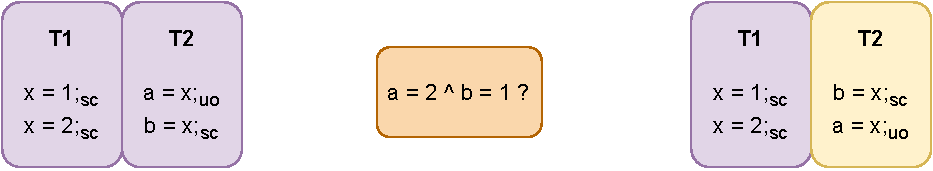
\includegraphics[scale=0.7]{5.InstructionReordering/0.Intro/ReorderingExample1(a).pdf}
            \caption{First example for reordering in candidates of the original program and its reordered counterpart.}
            \label{reord:example1(a)} 
        \end{figure}
        
        Figure~\ref{reord:example1(b)} has two sets of relations. 
        The first justifies the outcome for the reordered Candidate. 
        While the second justifies for the original Candidate. 
        Notice that in the first set of relations, we can infer that one may have a read memory ordered before a write that it reads from. 
        This is quite counter intuitive to understand at first. 
        But strictly from the semantics of the model, this justification to the observable behavior is completely valid\footnotemark. 
        \begin{figure}[H]
            \centering
            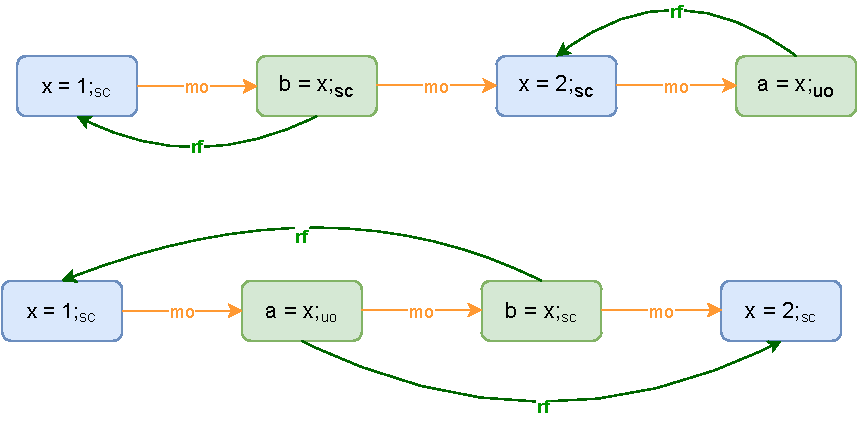
\includegraphics[scale=0.7]{5.InstructionReordering/0.Intro/ReorderingExample1(b).pdf}
            \caption{The set of partial order relations justifying the observable behavior in question for both the candidates in Figure~\ref{reord:example1(a)}.} 
            \label{reord:example1(b)}
        \end{figure}

        \footnotetext{In practice, this can be due to read speculation at the hardware level.}
        
        Consider another example in Figure~\ref{reord:example2(a)}.
        The figure on the left is the original candidate and that on the right is after reordering the two events of $T1$.
        The observable behavior in question is written in the middle(orange box). 
        \begin{figure}[H]
            \centering
            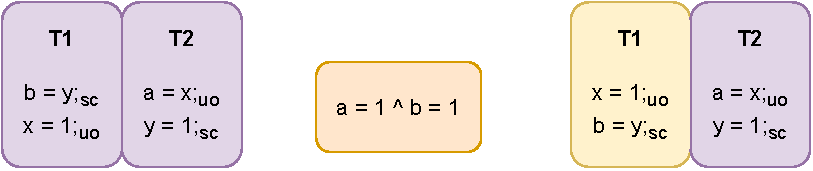
\includegraphics[scale=0.7]{5.InstructionReordering/0.Intro/ReorderingExample2(a).pdf}
            \caption{Second example for reordering with candidates of the original program and its reordered counterpart.} 
            \label{reord:example2(a)}
        \end{figure}
   
        Figure~\ref{reord:example2(b)} has two sets of relations. 
        The first justifies that such an outcome is not possible for the original program candidate due to Axiom \ref{CoRe}. 
        While the second justifies that this outcome is possible for the reordered program.
        Note that we cannot infer in the reordered candidate the set of relations for any candidate execution to have $\reln{a=x;_{uo}}{hb}{x=1;_{uo}}$. 
        \begin{figure}[H]
            \centering
            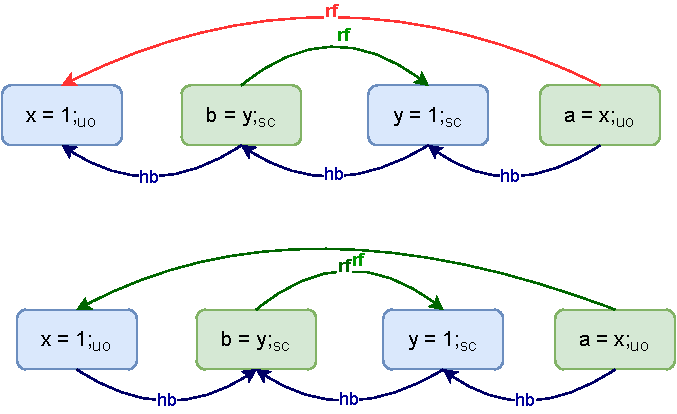
\includegraphics[scale=0.7]{5.InstructionReordering/0.Intro/ReorderingExample2(b).pdf}
            \caption{The set of partial order relations justifying the observable behavior in question for both the candidates in Figure~\ref{reord:example2(a)}.} 
            \label{reord:example2(b)}
        \end{figure}

        The above two examples show that we have to be careful while reordering two events in the same thread. 
        By example analysis, for each observable behavior, one must check all possible candidate executions and assert whether such an observable is possible or not. 
        This method of checking validity of reordering will scale exponentially as the program size increases. 
        It may also be the case that the compiler may not have information on which exact events would be executed in other threads to assert such reordering is valid. 

    
    
    
    
    

%Summary of Approach.
\section{Approach}

    We consider the same set of assumptions for reordering here. 
    Similar to reordering, our main objective is to ensure that the set of possible observable behaviors of a program, remain unchanged after elimination. 
    In the case of write elimination, the property we try to prove remains the same.
    In the case of read elimination though, we would want the observable behaviors excluding the specific read eliminated to be a subset.
    For both cases, if preserving all behaviors is not possible, then we would want the set of observable behaviors after elimination at the very least to be a subset.

    The main difference here is that elimination would remove certain happens-before relations, in contrast to having additional ones.
    From our point of view, we would want only the relations with the eliminated read/write to be removed after the transformation.
    The loss of these relations would certainly not have any new happens-before cycle introduced. 
    However, we still have to check whether the removed relations result in some new behavior. 
    We prove when it does not, by doing case-wise analysis on the type of relations eliminated.  

%Key definitions 
\section{Some Useful Definitions}
Before we go about proving when reordering is valid, we define certain helper definitions for it.

%Something we need to define for sake of proofs
\begin{definition}{Consecutive pair of events (\emph{cons})}
    \label{Cons}
    We define \emph{cons} as a function, which takes two events as input, and gives us a boolean indicating if they are consecutive pairs. Two events $e$ and $d$ are consecutive if they have a direct $\stck{_\textit{ao}}$ relation among them;  i.e those relations that are not derived through transitive property of $\stck{_\textit{hb}}$. 
    \begin{align*}
        (
        e \stck{_\textit{ao}} d  \ \wedge \ 
        \nexists k \ \textit{s.t.} \ 
        e \stck{_\textit{ao}} k  \ \wedge \
        k \stck{_\textit{ao}} d 
        )
        \ \vee \
        (
            d \stck{_\textit{ao}} e  \ \wedge \ 
            \nexists k \ \textit{s.t.} \ 
            d \stck{_\textit{ao}} k  \ \wedge \
            k \stck{_\textit{ao}} e  
        ).
    \end{align*}
\end{definition}

\begin{definition}{Direct happens-before relation (dir)}
    \label{Dir}
    We define \emph{dir} to take an ordered pair of events $(e,d)$ such that $\reln{e}{hb}{d}$ and gives a boolean value to indicate whether this relation is \textit{direct}, which can be formally stated as follows:
    \begin{align*}
        \nexists k \ \text{s.t.} \ \reln{e}{hb}{k} \wedge \reln{k}{hb}{d}.
    \end{align*}
    
    We can infer some useful things using \emph{dir} based on some information on events $e$ and $d$\footnotemark. 
    \begin{enumerate}
        \item If $\et{e}{uo}$, then $dir(e,d) \ \Rightarrow \ cons(e,d).$ 
        \item If $\et{d}{uo}$, then $dir(e,d) \ \Rightarrow \ cons(e,d).$
        \item If $\et{e}{sc}\ \wedge\ e\!\in\!R$, then $dir(e,d) \ \Rightarrow \ cons(e,d).$
        \item If $\et{e}{sc}\ \wedge\ e\!\in\!W$, then $dir(e,d) \ \Rightarrow \ cons(e,d)\ \vee\ \reln{e}{sw}{d}.$
        \item If $\et{d}{sc}\ \wedge\ d\!\in\!W$, then $dir(e,d) \ \Rightarrow \ cons(e,d).$
        \item If $\et{d}{sc}\ \wedge\ e\!\in\!R$, then $dir(e,d) \ \Rightarrow \ cons(e,d)\ \vee\ \reln{e}{sw}{d}.$
    \end{enumerate}

    \footnotetext{They can be proved trivially using definitions of $\stck{_{hb}}, \stck{_{sw}} \text{and} \stck{_{ao}}$}.
\end{definition}


\begin{definition}{Reorderable Pair (Reord)}
    \label{Reord}
    
    We define a boolean function \emph{Reord} that takes two ordered pair of events $(e,d)$ such that $\reln{e}{ao}{d}$ and gives a boolean value indicating if they are a reorderable pair\footnotemark.   
    \begin{align*}
        Reord(e,d) = \\
        (
        &((\et{e}{uo} \ \wedge \ \et{d}{uo}) \ \wedge \ 
                (   
                    (\event{e}{R} \ \wedge \ \event{d}{R}) \ \vee \ 
                    (\Re(e) \cap_\Re \Re(d) = \phi) 
                )
        ) \\ &\vee \\
        &((\et{e}{sc} \ \wedge \ \et{d}{uo}) \ \wedge \ 
                (
                    (\event{e}{W} \ \wedge \ (\Re(e) \cap_\Re \Re(d) = \phi)) 
                )
        ) \\ &\vee \\
        &((\et{e}{uo} \ \wedge \ \et{d}{sc}) \ \wedge \ 
                (
                    (\event{d}{R} \ \wedge \ (\Re(e) \cap_\Re \Re(d) = \phi)) 
                )
        )
        ).
    \end{align*}

    \footnotetext{We later prove that this exact definition defines when a pair of two consecutive events are reorderable.}
\end{definition}



%Key Lemmas 
This chapter addresses the validity of instruction reordering under the ECMAScript memory model.
We first start by showing some examples of Candidate Executions where reordering is not safe in the relaxed memory context.  
We give a brief summary of our approach towards a proof to identify when such a reordering is safe.
Next, we introduce a few more definitions for our purpose, followed by two lemmas that will be instrumental for proofs in this chapter and the next. 
We then formulate a theorem and a corresponding corollary that covers validity of reordering at a Candidate Execution level. 
Lastly, we address reordering at the program level involving conditional branching and loops.
We use counter examples to give a better intuitive understanding of the elements of the proof.
\ \newline
\ \newline  
\hrule 
\ \newline 
\ \newline 

\input{4.InstructionReordering/0.Intro/intro.tex}

%Summary of Approach.
\input{4.InstructionReordering/1.Approach.tex}

%Key definitions 
\input{4.InstructionReordering/2.Definitions.tex}

%Key Lemmas 
\input{4.InstructionReordering/3.Lemmas/main.tex}

%Valid reordering at the Candidate Execution level
\input{4.InstructionReordering/4.ValidReorderingCandidate/main.tex}

%From Candidates to Programs
\input{4.InstructionReordering/5.ValidReorderingProgram/main.tex}

%Conclusion (write here itself. No need for a new .tex file)
\ \newline
\ \newline  
\hrule 
\ \newline 
\ \newline 
To summarize, this chapter addressed the validity of instruction reordering under the ECMAScript Memory Model. 
We first built a conservative proof for reordering based on candidate executions.
We later extended it to programs abstracted to the set of shared memory events. 
We discussed throughout the limitation and advantages of our conservative approach. 
We also presented examples throughout this chapter to get a fair intuitive understanding of the ideas behind the proof and the role of the axiomatic model in it.
In the next chapter, we will address the validity of elimination under the ECMAScript Memory Model.

%Valid reordering at the Candidate Execution level
This chapter addresses the validity of instruction reordering under the ECMAScript memory model.
We first start by showing some examples of Candidate Executions where reordering is not safe in the relaxed memory context.  
We give a brief summary of our approach towards a proof to identify when such a reordering is safe.
Next, we introduce a few more definitions for our purpose, followed by two lemmas that will be instrumental for proofs in this chapter and the next. 
We then formulate a theorem and a corresponding corollary that covers validity of reordering at a Candidate Execution level. 
Lastly, we address reordering at the program level involving conditional branching and loops.
We use counter examples to give a better intuitive understanding of the elements of the proof.
\ \newline
\ \newline  
\hrule 
\ \newline 
\ \newline 

\input{4.InstructionReordering/0.Intro/intro.tex}

%Summary of Approach.
\input{4.InstructionReordering/1.Approach.tex}

%Key definitions 
\input{4.InstructionReordering/2.Definitions.tex}

%Key Lemmas 
\input{4.InstructionReordering/3.Lemmas/main.tex}

%Valid reordering at the Candidate Execution level
\input{4.InstructionReordering/4.ValidReorderingCandidate/main.tex}

%From Candidates to Programs
\input{4.InstructionReordering/5.ValidReorderingProgram/main.tex}

%Conclusion (write here itself. No need for a new .tex file)
\ \newline
\ \newline  
\hrule 
\ \newline 
\ \newline 
To summarize, this chapter addressed the validity of instruction reordering under the ECMAScript Memory Model. 
We first built a conservative proof for reordering based on candidate executions.
We later extended it to programs abstracted to the set of shared memory events. 
We discussed throughout the limitation and advantages of our conservative approach. 
We also presented examples throughout this chapter to get a fair intuitive understanding of the ideas behind the proof and the role of the axiomatic model in it.
In the next chapter, we will address the validity of elimination under the ECMAScript Memory Model.

%From Candidates to Programs
This chapter addresses the validity of instruction reordering under the ECMAScript memory model.
We first start by showing some examples of Candidate Executions where reordering is not safe in the relaxed memory context.  
We give a brief summary of our approach towards a proof to identify when such a reordering is safe.
Next, we introduce a few more definitions for our purpose, followed by two lemmas that will be instrumental for proofs in this chapter and the next. 
We then formulate a theorem and a corresponding corollary that covers validity of reordering at a Candidate Execution level. 
Lastly, we address reordering at the program level involving conditional branching and loops.
We use counter examples to give a better intuitive understanding of the elements of the proof.
\ \newline
\ \newline  
\hrule 
\ \newline 
\ \newline 

\input{4.InstructionReordering/0.Intro/intro.tex}

%Summary of Approach.
\input{4.InstructionReordering/1.Approach.tex}

%Key definitions 
\input{4.InstructionReordering/2.Definitions.tex}

%Key Lemmas 
\input{4.InstructionReordering/3.Lemmas/main.tex}

%Valid reordering at the Candidate Execution level
\input{4.InstructionReordering/4.ValidReorderingCandidate/main.tex}

%From Candidates to Programs
\input{4.InstructionReordering/5.ValidReorderingProgram/main.tex}

%Conclusion (write here itself. No need for a new .tex file)
\ \newline
\ \newline  
\hrule 
\ \newline 
\ \newline 
To summarize, this chapter addressed the validity of instruction reordering under the ECMAScript Memory Model. 
We first built a conservative proof for reordering based on candidate executions.
We later extended it to programs abstracted to the set of shared memory events. 
We discussed throughout the limitation and advantages of our conservative approach. 
We also presented examples throughout this chapter to get a fair intuitive understanding of the ideas behind the proof and the role of the axiomatic model in it.
In the next chapter, we will address the validity of elimination under the ECMAScript Memory Model.

%Conclusion (write here itself. No need for a new .tex file)
\ \newline
\ \newline  
\hrule 
\ \newline 
\ \newline 
To summarize, this chapter addressed the validity of instruction reordering under the ECMAScript Memory Model. 
We first built a conservative proof for reordering based on candidate executions.
We later extended it to programs abstracted to the set of shared memory events. 
We discussed throughout the limitation and advantages of our conservative approach. 
We also presented examples throughout this chapter to get a fair intuitive understanding of the ideas behind the proof and the role of the axiomatic model in it.
In the next chapter, we will address the validity of elimination under the ECMAScript Memory Model.

%From Candidates to Programs
This chapter addresses the validity of instruction reordering under the ECMAScript memory model.
We first start by showing some examples of Candidate Executions where reordering is not safe in the relaxed memory context.  
We give a brief summary of our approach towards a proof to identify when such a reordering is safe.
Next, we introduce a few more definitions for our purpose, followed by two lemmas that will be instrumental for proofs in this chapter and the next. 
We then formulate a theorem and a corresponding corollary that covers validity of reordering at a Candidate Execution level. 
Lastly, we address reordering at the program level involving conditional branching and loops.
We use counter examples to give a better intuitive understanding of the elements of the proof.
\ \newline
\ \newline  
\hrule 
\ \newline 
\ \newline 


\section{Introduction}
    Instruction reordering is a common transformation done by the compiler/hardware, which is essential to optimizations such as instruction scheduling, loop invariant removal, partial redundancy elimination, etc. 
    However, whether we can do such reordering freely given a concurrent program using relaxed memory accesses is a bit unclear. 
     
    \paragraph{Simple reordering is not straightforward under shared memory semantics}
    The main reason is that memory accesses here, do not just perform the desired operation (i.e Read / Write) but also imply certain visibility guarantees across all the other threads.  
    In our observation, we find that, the relaxed memory model of ECMAScript prescribe semantics for visibility using the $\stck{_{hb}}$ relations. 
    
    \paragraph{Some Examples}
        We show a couple of examples to showcase why reordering may not be that straightforward. 
        Consider the first example in Figure~\ref{reord:example1(a)} below of a Candidate before and after reordering two events.
        The original candidate is to the left and that on the right is after reordering the two reads of $T2$.
        The observable behavior in question is written in the middle(orange box). 
        \begin{figure}[H]
            \centering
            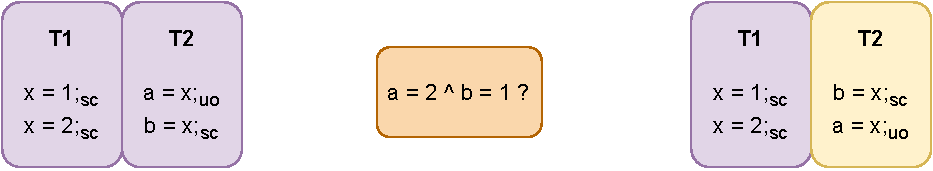
\includegraphics[scale=0.7]{5.InstructionReordering/0.Intro/ReorderingExample1(a).pdf}
            \caption{First example for reordering in candidates of the original program and its reordered counterpart.}
            \label{reord:example1(a)} 
        \end{figure}
        
        Figure~\ref{reord:example1(b)} has two sets of relations. 
        The first justifies the outcome for the reordered Candidate. 
        While the second justifies for the original Candidate. 
        Notice that in the first set of relations, we can infer that one may have a read memory ordered before a write that it reads from. 
        This is quite counter intuitive to understand at first. 
        But strictly from the semantics of the model, this justification to the observable behavior is completely valid\footnotemark. 
        \begin{figure}[H]
            \centering
            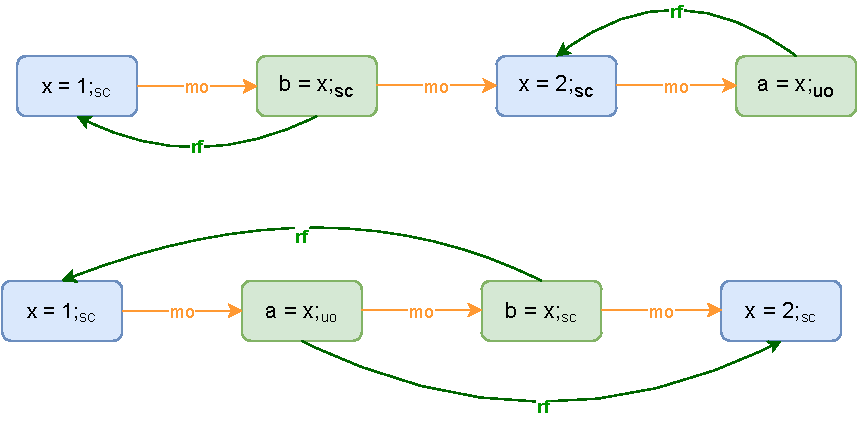
\includegraphics[scale=0.7]{5.InstructionReordering/0.Intro/ReorderingExample1(b).pdf}
            \caption{The set of partial order relations justifying the observable behavior in question for both the candidates in Figure~\ref{reord:example1(a)}.} 
            \label{reord:example1(b)}
        \end{figure}

        \footnotetext{In practice, this can be due to read speculation at the hardware level.}
        
        Consider another example in Figure~\ref{reord:example2(a)}.
        The figure on the left is the original candidate and that on the right is after reordering the two events of $T1$.
        The observable behavior in question is written in the middle(orange box). 
        \begin{figure}[H]
            \centering
            \includegraphics[scale=0.7]{5.InstructionReordering/0.Intro/ReorderingExample2(a).pdf}
            \caption{Second example for reordering with candidates of the original program and its reordered counterpart.} 
            \label{reord:example2(a)}
        \end{figure}
   
        Figure~\ref{reord:example2(b)} has two sets of relations. 
        The first justifies that such an outcome is not possible for the original program candidate due to Axiom \ref{CoRe}. 
        While the second justifies that this outcome is possible for the reordered program.
        Note that we cannot infer in the reordered candidate the set of relations for any candidate execution to have $\reln{a=x;_{uo}}{hb}{x=1;_{uo}}$. 
        \begin{figure}[H]
            \centering
            \includegraphics[scale=0.7]{5.InstructionReordering/0.Intro/ReorderingExample2(b).pdf}
            \caption{The set of partial order relations justifying the observable behavior in question for both the candidates in Figure~\ref{reord:example2(a)}.} 
            \label{reord:example2(b)}
        \end{figure}

        The above two examples show that we have to be careful while reordering two events in the same thread. 
        By example analysis, for each observable behavior, one must check all possible candidate executions and assert whether such an observable is possible or not. 
        This method of checking validity of reordering will scale exponentially as the program size increases. 
        It may also be the case that the compiler may not have information on which exact events would be executed in other threads to assert such reordering is valid. 

    
    
    
    
    

%Summary of Approach.
\section{Approach}

    We consider the same set of assumptions for reordering here. 
    Similar to reordering, our main objective is to ensure that the set of possible observable behaviors of a program, remain unchanged after elimination. 
    In the case of write elimination, the property we try to prove remains the same.
    In the case of read elimination though, we would want the observable behaviors excluding the specific read eliminated to be a subset.
    For both cases, if preserving all behaviors is not possible, then we would want the set of observable behaviors after elimination at the very least to be a subset.

    The main difference here is that elimination would remove certain happens-before relations, in contrast to having additional ones.
    From our point of view, we would want only the relations with the eliminated read/write to be removed after the transformation.
    The loss of these relations would certainly not have any new happens-before cycle introduced. 
    However, we still have to check whether the removed relations result in some new behavior. 
    We prove when it does not, by doing case-wise analysis on the type of relations eliminated.  

%Key definitions 
\section{Some Useful Definitions}
Before we go about proving when reordering is valid, we define certain helper definitions for it.

%Something we need to define for sake of proofs
\begin{definition}{Consecutive pair of events (\emph{cons})}
    \label{Cons}
    We define \emph{cons} as a function, which takes two events as input, and gives us a boolean indicating if they are consecutive pairs. Two events $e$ and $d$ are consecutive if they have a direct $\stck{_\textit{ao}}$ relation among them;  i.e those relations that are not derived through transitive property of $\stck{_\textit{hb}}$. 
    \begin{align*}
        (
        e \stck{_\textit{ao}} d  \ \wedge \ 
        \nexists k \ \textit{s.t.} \ 
        e \stck{_\textit{ao}} k  \ \wedge \
        k \stck{_\textit{ao}} d 
        )
        \ \vee \
        (
            d \stck{_\textit{ao}} e  \ \wedge \ 
            \nexists k \ \textit{s.t.} \ 
            d \stck{_\textit{ao}} k  \ \wedge \
            k \stck{_\textit{ao}} e  
        ).
    \end{align*}
\end{definition}

\begin{definition}{Direct happens-before relation (dir)}
    \label{Dir}
    We define \emph{dir} to take an ordered pair of events $(e,d)$ such that $\reln{e}{hb}{d}$ and gives a boolean value to indicate whether this relation is \textit{direct}, which can be formally stated as follows:
    \begin{align*}
        \nexists k \ \text{s.t.} \ \reln{e}{hb}{k} \wedge \reln{k}{hb}{d}.
    \end{align*}
    
    We can infer some useful things using \emph{dir} based on some information on events $e$ and $d$\footnotemark. 
    \begin{enumerate}
        \item If $\et{e}{uo}$, then $dir(e,d) \ \Rightarrow \ cons(e,d).$ 
        \item If $\et{d}{uo}$, then $dir(e,d) \ \Rightarrow \ cons(e,d).$
        \item If $\et{e}{sc}\ \wedge\ e\!\in\!R$, then $dir(e,d) \ \Rightarrow \ cons(e,d).$
        \item If $\et{e}{sc}\ \wedge\ e\!\in\!W$, then $dir(e,d) \ \Rightarrow \ cons(e,d)\ \vee\ \reln{e}{sw}{d}.$
        \item If $\et{d}{sc}\ \wedge\ d\!\in\!W$, then $dir(e,d) \ \Rightarrow \ cons(e,d).$
        \item If $\et{d}{sc}\ \wedge\ e\!\in\!R$, then $dir(e,d) \ \Rightarrow \ cons(e,d)\ \vee\ \reln{e}{sw}{d}.$
    \end{enumerate}

    \footnotetext{They can be proved trivially using definitions of $\stck{_{hb}}, \stck{_{sw}} \text{and} \stck{_{ao}}$}.
\end{definition}


\begin{definition}{Reorderable Pair (Reord)}
    \label{Reord}
    
    We define a boolean function \emph{Reord} that takes two ordered pair of events $(e,d)$ such that $\reln{e}{ao}{d}$ and gives a boolean value indicating if they are a reorderable pair\footnotemark.   
    \begin{align*}
        Reord(e,d) = \\
        (
        &((\et{e}{uo} \ \wedge \ \et{d}{uo}) \ \wedge \ 
                (   
                    (\event{e}{R} \ \wedge \ \event{d}{R}) \ \vee \ 
                    (\Re(e) \cap_\Re \Re(d) = \phi) 
                )
        ) \\ &\vee \\
        &((\et{e}{sc} \ \wedge \ \et{d}{uo}) \ \wedge \ 
                (
                    (\event{e}{W} \ \wedge \ (\Re(e) \cap_\Re \Re(d) = \phi)) 
                )
        ) \\ &\vee \\
        &((\et{e}{uo} \ \wedge \ \et{d}{sc}) \ \wedge \ 
                (
                    (\event{d}{R} \ \wedge \ (\Re(e) \cap_\Re \Re(d) = \phi)) 
                )
        )
        ).
    \end{align*}

    \footnotetext{We later prove that this exact definition defines when a pair of two consecutive events are reorderable.}
\end{definition}



%Key Lemmas 
This chapter addresses the validity of instruction reordering under the ECMAScript memory model.
We first start by showing some examples of Candidate Executions where reordering is not safe in the relaxed memory context.  
We give a brief summary of our approach towards a proof to identify when such a reordering is safe.
Next, we introduce a few more definitions for our purpose, followed by two lemmas that will be instrumental for proofs in this chapter and the next. 
We then formulate a theorem and a corresponding corollary that covers validity of reordering at a Candidate Execution level. 
Lastly, we address reordering at the program level involving conditional branching and loops.
We use counter examples to give a better intuitive understanding of the elements of the proof.
\ \newline
\ \newline  
\hrule 
\ \newline 
\ \newline 

\input{4.InstructionReordering/0.Intro/intro.tex}

%Summary of Approach.
\input{4.InstructionReordering/1.Approach.tex}

%Key definitions 
\input{4.InstructionReordering/2.Definitions.tex}

%Key Lemmas 
\input{4.InstructionReordering/3.Lemmas/main.tex}

%Valid reordering at the Candidate Execution level
\input{4.InstructionReordering/4.ValidReorderingCandidate/main.tex}

%From Candidates to Programs
\input{4.InstructionReordering/5.ValidReorderingProgram/main.tex}

%Conclusion (write here itself. No need for a new .tex file)
\ \newline
\ \newline  
\hrule 
\ \newline 
\ \newline 
To summarize, this chapter addressed the validity of instruction reordering under the ECMAScript Memory Model. 
We first built a conservative proof for reordering based on candidate executions.
We later extended it to programs abstracted to the set of shared memory events. 
We discussed throughout the limitation and advantages of our conservative approach. 
We also presented examples throughout this chapter to get a fair intuitive understanding of the ideas behind the proof and the role of the axiomatic model in it.
In the next chapter, we will address the validity of elimination under the ECMAScript Memory Model.

%Valid reordering at the Candidate Execution level
This chapter addresses the validity of instruction reordering under the ECMAScript memory model.
We first start by showing some examples of Candidate Executions where reordering is not safe in the relaxed memory context.  
We give a brief summary of our approach towards a proof to identify when such a reordering is safe.
Next, we introduce a few more definitions for our purpose, followed by two lemmas that will be instrumental for proofs in this chapter and the next. 
We then formulate a theorem and a corresponding corollary that covers validity of reordering at a Candidate Execution level. 
Lastly, we address reordering at the program level involving conditional branching and loops.
We use counter examples to give a better intuitive understanding of the elements of the proof.
\ \newline
\ \newline  
\hrule 
\ \newline 
\ \newline 

\input{4.InstructionReordering/0.Intro/intro.tex}

%Summary of Approach.
\input{4.InstructionReordering/1.Approach.tex}

%Key definitions 
\input{4.InstructionReordering/2.Definitions.tex}

%Key Lemmas 
\input{4.InstructionReordering/3.Lemmas/main.tex}

%Valid reordering at the Candidate Execution level
\input{4.InstructionReordering/4.ValidReorderingCandidate/main.tex}

%From Candidates to Programs
\input{4.InstructionReordering/5.ValidReorderingProgram/main.tex}

%Conclusion (write here itself. No need for a new .tex file)
\ \newline
\ \newline  
\hrule 
\ \newline 
\ \newline 
To summarize, this chapter addressed the validity of instruction reordering under the ECMAScript Memory Model. 
We first built a conservative proof for reordering based on candidate executions.
We later extended it to programs abstracted to the set of shared memory events. 
We discussed throughout the limitation and advantages of our conservative approach. 
We also presented examples throughout this chapter to get a fair intuitive understanding of the ideas behind the proof and the role of the axiomatic model in it.
In the next chapter, we will address the validity of elimination under the ECMAScript Memory Model.

%From Candidates to Programs
This chapter addresses the validity of instruction reordering under the ECMAScript memory model.
We first start by showing some examples of Candidate Executions where reordering is not safe in the relaxed memory context.  
We give a brief summary of our approach towards a proof to identify when such a reordering is safe.
Next, we introduce a few more definitions for our purpose, followed by two lemmas that will be instrumental for proofs in this chapter and the next. 
We then formulate a theorem and a corresponding corollary that covers validity of reordering at a Candidate Execution level. 
Lastly, we address reordering at the program level involving conditional branching and loops.
We use counter examples to give a better intuitive understanding of the elements of the proof.
\ \newline
\ \newline  
\hrule 
\ \newline 
\ \newline 

\input{4.InstructionReordering/0.Intro/intro.tex}

%Summary of Approach.
\input{4.InstructionReordering/1.Approach.tex}

%Key definitions 
\input{4.InstructionReordering/2.Definitions.tex}

%Key Lemmas 
\input{4.InstructionReordering/3.Lemmas/main.tex}

%Valid reordering at the Candidate Execution level
\input{4.InstructionReordering/4.ValidReorderingCandidate/main.tex}

%From Candidates to Programs
\input{4.InstructionReordering/5.ValidReorderingProgram/main.tex}

%Conclusion (write here itself. No need for a new .tex file)
\ \newline
\ \newline  
\hrule 
\ \newline 
\ \newline 
To summarize, this chapter addressed the validity of instruction reordering under the ECMAScript Memory Model. 
We first built a conservative proof for reordering based on candidate executions.
We later extended it to programs abstracted to the set of shared memory events. 
We discussed throughout the limitation and advantages of our conservative approach. 
We also presented examples throughout this chapter to get a fair intuitive understanding of the ideas behind the proof and the role of the axiomatic model in it.
In the next chapter, we will address the validity of elimination under the ECMAScript Memory Model.

%Conclusion (write here itself. No need for a new .tex file)
\ \newline
\ \newline  
\hrule 
\ \newline 
\ \newline 
To summarize, this chapter addressed the validity of instruction reordering under the ECMAScript Memory Model. 
We first built a conservative proof for reordering based on candidate executions.
We later extended it to programs abstracted to the set of shared memory events. 
We discussed throughout the limitation and advantages of our conservative approach. 
We also presented examples throughout this chapter to get a fair intuitive understanding of the ideas behind the proof and the role of the axiomatic model in it.
In the next chapter, we will address the validity of elimination under the ECMAScript Memory Model.

%Conclusion (write here itself. No need for a new .tex file)
\ \newline
\ \newline  
\hrule 
\ \newline 
\ \newline 
To summarize, this chapter addressed the validity of instruction reordering under the ECMAScript Memory Model. 
We first built a conservative proof for reordering based on candidate executions.
We later extended it to programs abstracted to the set of shared memory events. 
We discussed throughout the limitation and advantages of our conservative approach. 
We also presented examples throughout this chapter to get a fair intuitive understanding of the ideas behind the proof and the role of the axiomatic model in it.
In the next chapter, we will address the validity of elimination under the ECMAScript Memory Model.

%Conclusion (write here itself. No need for a new .tex file)
\ \newline
\ \newline  
\hrule 
\ \newline 
\ \newline 
To summarize, this chapter addressed the validity of instruction reordering under the ECMAScript Memory Model. 
We first built a conservative proof for reordering based on candidate executions.
We later extended it to programs abstracted to the set of shared memory events. 
We discussed throughout the limitation and advantages of our conservative approach. 
We also presented examples throughout this chapter to get a fair intuitive understanding of the ideas behind the proof and the role of the axiomatic model in it.
In the next chapter, we will address the validity of elimination under the ECMAScript Memory Model.